\documentclass[]{article}
\usepackage{lmodern}
\usepackage{amssymb,amsmath}
\usepackage{ifxetex,ifluatex}
\usepackage{fixltx2e} % provides \textsubscript
\ifnum 0\ifxetex 1\fi\ifluatex 1\fi=0 % if pdftex
  \usepackage[T1]{fontenc}
  \usepackage[utf8]{inputenc}
\else % if luatex or xelatex
  \ifxetex
    \usepackage{mathspec}
  \else
    \usepackage{fontspec}
  \fi
  \defaultfontfeatures{Ligatures=TeX,Scale=MatchLowercase}
\fi
% use upquote if available, for straight quotes in verbatim environments
\IfFileExists{upquote.sty}{\usepackage{upquote}}{}
% use microtype if available
\IfFileExists{microtype.sty}{%
\usepackage{microtype}
\UseMicrotypeSet[protrusion]{basicmath} % disable protrusion for tt fonts
}{}
\usepackage[margin=1in]{geometry}
\usepackage{hyperref}
\hypersetup{unicode=true,
            pdftitle={Einfache Korpusanalysen: Ein Schnelleinstieg},
            pdfauthor={Stefan Hartmann},
            pdfborder={0 0 0},
            breaklinks=true}
\urlstyle{same}  % don't use monospace font for urls
\usepackage{longtable,booktabs}
\usepackage{graphicx,grffile}
\makeatletter
\def\maxwidth{\ifdim\Gin@nat@width>\linewidth\linewidth\else\Gin@nat@width\fi}
\def\maxheight{\ifdim\Gin@nat@height>\textheight\textheight\else\Gin@nat@height\fi}
\makeatother
% Scale images if necessary, so that they will not overflow the page
% margins by default, and it is still possible to overwrite the defaults
% using explicit options in \includegraphics[width, height, ...]{}
\setkeys{Gin}{width=\maxwidth,height=\maxheight,keepaspectratio}
\IfFileExists{parskip.sty}{%
\usepackage{parskip}
}{% else
\setlength{\parindent}{0pt}
\setlength{\parskip}{6pt plus 2pt minus 1pt}
}
\setlength{\emergencystretch}{3em}  % prevent overfull lines
\providecommand{\tightlist}{%
  \setlength{\itemsep}{0pt}\setlength{\parskip}{0pt}}
\setcounter{secnumdepth}{5}
% Redefines (sub)paragraphs to behave more like sections
\ifx\paragraph\undefined\else
\let\oldparagraph\paragraph
\renewcommand{\paragraph}[1]{\oldparagraph{#1}\mbox{}}
\fi
\ifx\subparagraph\undefined\else
\let\oldsubparagraph\subparagraph
\renewcommand{\subparagraph}[1]{\oldsubparagraph{#1}\mbox{}}
\fi

%%% Use protect on footnotes to avoid problems with footnotes in titles
\let\rmarkdownfootnote\footnote%
\def\footnote{\protect\rmarkdownfootnote}

%%% Change title format to be more compact
\usepackage{titling}

% Create subtitle command for use in maketitle
\providecommand{\subtitle}[1]{
  \posttitle{
    \begin{center}\large#1\end{center}
    }
}

\setlength{\droptitle}{-2em}

  \title{Einfache Korpusanalysen: Ein Schnelleinstieg}
    \pretitle{\vspace{\droptitle}\centering\huge}
  \posttitle{\par}
    \author{Stefan Hartmann}
    \preauthor{\centering\large\emph}
  \postauthor{\par}
      \predate{\centering\large\emph}
  \postdate{\par}
    \date{2019-06-14}

\usepackage[none]{hyphenat}
\usepackage[german]{babel}
\usepackage[autostyle,german=quotes]{csquotes}

\renewcommand{\figurename}{Fig.}
\renewcommand{\contentsname}{Inhalt}

\begin{document}
\maketitle

{
\setcounter{tocdepth}{4}
\tableofcontents
}
\section{Einstieg}\label{einstieg}

Ziel dieses Tutorials ist es, Anfänger*innen einen möglichst
niedrigschwelligen Einstieg in einfache Korpusanalysen zu ermöglichen.
Es ist insbesondere für Studierende gedacht, die z.B. für eine
Seminararbeit eine Korpusrecherche durchführen möchten, aber bislang
noch keine praktische Erfahrung mit korpuslinguistischen Methoden
sammeln konnten. Das Tutorial bietet anhand eines konkreten Beispiels
eine Schritt-für-Schritt-Anleitung, wie man von der Fragestellung zur
Datengewinnung hin zur Analyse der Daten gelangen kann. Dabei nutzen wir
folgende Ressourcen bzw. Programme:

\begin{itemize}
\item
  Das Kernkorpus des 20. Jahrhunderts des Digitalen Wörterbuchs der
  Deutschen Sprache, verfügbar über dwds.de.
\item
  ein Tabellenkalkulationsprogramm, wobei alle wesentlichen
  Arbeitsschritte sowohl für Microsoft Excel als auch für die kostenlose
  Alternative LibreOffice Calc beschrieben werden. Es genügt natürlich,
  wenn Sie mit einem der beiden Programme arbeiten; die Abschnitte zum
  jeweils anderen Programm können Sie dann getrost überspringen.
\end{itemize}

Um wirklich einen Schnelleinstieg bieten zu können, muss ich
notwendigerweise vieles vereinfachen. Für Ihre konkrete Korpusstudie
werden Sie daher wahrscheinlich nicht umhinkommen, sich an der einen
oder anderen Stelle tiefer einzulesen. Dafür verweise ich im Text
gelegentlich auf weiterführende Ressourcen. Teilweise finden sich auch
in diesem Tutorial vertiefende Passagen, die Sie (in der HTML-Version)
aufklappen können:

 ‣ \textbf{klick mich}

Hallo, ich bin eine vertiefende Passage.

Sonst gibt es hier nichts zu sehen. Sie können mich gern wieder
schließen. Danke.

Ein Hinweis vorab: Das Tutorial setzt keine Kenntnisse in der
Korpuslinguistik oder im Umgang mit Tabellenkalkulationsprogrammen
voraus, wohl aber grammatische Grundkenntnisse. Sollten Sie die
Fachbegriffe nicht verstehen, empfehle ich sehr, sie nachzuschlagen und
die entsprechenden Wissenslücken zu schließen.

Und noch ein Hinweis: Das Tutorial liegt sowohl im HTML-Format als auch
im PDF-Format vor (die PDF-Version können Sie im HTML-Dokument durch
Klick auf den PDF-Button ganz oben herunterladen). Die HTML-Version
arbeitet viel mit animierten GIFs, die in der PDF-Version natürlich
nicht zu sehen sind. Dafür benötigt die PDF-Version weit weniger
Speicherplatz.

Ein letzter Hinweis: Da ich aus Gründen, die hier auszuführen zu viel
Platz wegnehmen würde, mit den englischen Versionen von Excel und Calc
arbeite, sehen Sie in den Screenshots und Screencasts immer die
englischen Varianten der einschlägigen Befehle. Im Text nenne ich
teilweise die deutsche Übersetzung, ohne aber in jedem Einzelfall
geprüft zu haben, ob das auch wirklich die Übersetzung ist, die in den
deutschen Versionen der Programme verwendet wird.

\begin{center}
\includegraphics[width=0.3\linewidth,height=0.3\textheight]{docs/fig/by-sa} \end{center}

Dieses Tutorial wurde mit Hilfe von Bookdown für R geschrieben und
publiziert. Es ist lizenziert unter CC-BY-SA und kann gerne mit
Quellenangabe weitergegeben und adaptiert werden.

Zitiervorschlag: Hartmann, Stefan. 2019. Einfache Korpusanalysen: Ein
Schnelleinstieg.
\url{https://empirical-linguistics.github.io/korpus-schnelleinstieg/}.
doi 10.5281/zenodo.3246336.

\section{Von der Fragestellung zur
Konkordanz}\label{von-der-fragestellung-zur-konkordanz}

Die meisten empirischen Studien lassen sich auf folgende Schritte
herunterbrechen:

\begin{itemize}
\tightlist
\item
  Eine Fragestellung formulieren
\item
  Daten erheben
\item
  Daten auswerten.
\end{itemize}

\subsection{Eine Fragestellung
formulieren}\label{eine-fragestellung-formulieren}

Der erste Schritt ist wahrscheinlich der wichtigste. Nur wenn Sie eine
gute Forschungsfrage haben, können Sie eine aussagekräftige empirische
Analyse durchführen. Aus der Forschungsfrage ergibt sich die Methode:
Für manche Fragestellungen bietet sich z.B. eine Fragebogenstudie an,
für andere eine psycho- oder neurolinguistische Herangehensweise, für
wieder andere eine Korpusrecherche.

Das heißt auch: Wenn Sie eine Korpusanalyse durchführen möchten,
brauchen Sie eine Fragestellung, die korpuslinguistisch
operationalisierbar ist. Beispielsweise lässt sich eine Frage wie
\enquote{Welche Gehirnareale werden beim Hören von Bewegungsverben
aktiviert?} natürlich nicht mit Hilfe von Korpusdaten beantworten.

Für unsere Beispielanalyse werfen wir einen Blick auf die prädikative
Verwendung der Partizipien \emph{programmiert} und
\emph{vorprogrammiert}. Letzteres ist manchen Sprachpflegern ein Dorn im
Auge: So bezeichnet es Batian Sick als

\begin{quote}
\enquote{umgangssprachliches Blähwort, über das schon Heerscharen von
Sprachpflegern hergefallen sind -- vergebens, denn es wird immer munter
weiter vorprogrammiert. Dabei wissen nicht nur Programmierer: Man
programmiert immer im Voraus, die Vorsilbe vor- ist daher pleonastisch,
zu Deutsch: doppelt gemoppelt.} \hfill ---
\url{https://bastiansick.de/kolumnen/abc/vorprogrammiertprogrammiert/}
\end{quote}

Was Sprachpfleger wie Sick jedoch oft verkennen, ist, dass Sprache nicht
immer \enquote{logisch} ist. Vielmehr suchen sich Wörter oft eigene
Nischen. Beispielsweise ist mein Bürostuhl kein \emph{Rollstuhl}, obwohl
er Rollen hat -- denn das Wort \emph{Rollstuhl} hat eine eigene
Bedeutung angenommen, die sich nicht kompositional aus seinen
Einzelteilen ergibt. Im Falle von \emph{vorprogrammiert} hingegen passt
zwar die Paraphrase \enquote{im Voraus programmiert}. Aber trotzdem wäre
denkbar, dass das Wort eine Spezialisierung erfahren hat: Wird
\emph{programmiert} möglicherweise eher dann verwendet, wenn ein
Programmierungsvorgang im wörtlichen Sinn gemeint ist, und
\emph{vorprogrammiert} eher dann, wenn ein z.B. ein Skandal oder eine
Katastrophe \enquote{vorprogrammiert} sind? Das ist die Fragestellung,
der wir im Folgenden nachgehen möchten.

 ‣ \textbf{Fragestellungen und Hypothesen}

Die Unterscheidung von \textbf{Fragestellung} und \textbf{Hypothese}
bereitet Anfänger*innen oft Schwierigkeiten. Beide hängen eng zusammen.
In unserem Beispiel könnte man die Frage in eine Hypothese
umformulieren: \enquote{vorprogrammiert wird eher in metaphorischem und
programmiert eher im wörtlichen Sinn verwendet.}

Hypothesen ergeben sich in der Regel aus konkreten Fragestellungen.
Beispielsweise könnte in einer soziologischen oder
politikwissenschaftlichen Studie die Fragestellung lauten: Welchen
Einfluss hat das Alter auf das Wahlverhalten in Deutschland? Da man zu
diesem Themengebiet aus der bisherigen Forschung und aus der
Alltagserfahrung das eine oder andere schon weiß, kann man begründete
Annahmen darüber treffen, wie die Antwort auf diese Frage aussieht. So
könnte man davon ausgehen, dass z.B. ältere Menschen eher etablierte und
vielleicht auch eher konservative Parteien wählen und dass außerdem bei
Älteren eine höhere Wahlbeteiligung vorliegt. Diese Annahmen nennt man
Hypothesen. Sie werden auf Grundlage der Daten, die man erhebt,
überprüft.

Nicht immer ist es möglich oder notwendig, konkrete Hypothesen zu
formulieren. Gerade bei Phänomenen, über die noch sehr wenig bekannt
ist, bietet es sich manchmal an, \textbf{explorativ}, also
\enquote{erkundend}, zu arbeiten. Auch dann gehe ich mit einer
Fragestellung an meine Daten heran, ohne jedoch im Voraus eine Erwartung
zu haben, wie die Antwort auf meine Frage aussehen wird.

\subsection{Daten erheben}\label{daten-erheben}

\subsubsection{Suchsyntax}\label{suchsyntax}

Für die Datenerhebung verwenden wir das DWDS-Kernkorpus des 20.
Jahrhunderts, das über dwds.de zugänglich ist. Wir suchen auf der
Wortebene mit Hilfe von regulären Ausdrücken nach den Formen
\emph{programmiert} und \emph{vorprogrammiert}. Dafür benutzen wir den
Suchstring
\texttt{@programmiert\ \textbar{}\textbar{}\ @vorprogrammiert}. Das
@-Zeichen bedeutet, dass wir genau diese Strings suchen und keine
anderen Wortformen wie \emph{programmierte}, \emph{programmiertes} etc.
Da uns nur die prädikative Verwendung interessiert, brauchen wir die
flektierten Wortformen nicht. Der horizontale Strich \textbar{} ist der
ODER-Operator; dass man ihn hier doppelt setzen muss, ist eine
Besonderheit der DWDS-Suchsyntax.

‣ \textbf{Alternative Suchabfrage mit regulären Ausdrücken}

Alternativ können wir das gleiche Ergebnis auch durch Verwendug
regulärer Ausdrücke erzielen: \texttt{\$w=/(vor)?programmiert/g}. Ich
ermutige alle, die sich mit Korpuslinguistik beschäftigen wollen, sehr,
sich mit regulären Ausdrücken vertraut zu machen. Allerdings unterstützt
die DWDS-Suchsyntax reguläre Ausdrücke derzeit nur in sehr beschränktem
Maße. (Deutlich besser ist in dieser Hinsicht das alternative
Abfrageportal Dstar, das jedoch für Anfänger*innen nur bedingt geeignet
ist.)

 ‣ \textbf{Zur Suche im DWDS und anderswo} - Die Hilfe zur Suche im DWDS
findet sich hier.

\begin{itemize}
\item
  Einen Einstieg in reguläre Ausdrücke bietet z.B.
  regular-expressions.info.
\item
  In den Begleitmaterialien zu meiner \enquote{Deutschen
  Sprachgeschichte} finden sich ebenfalls einige Tutorials zur Suche in
  einschlägigen Korpora.
\item
  Sehr empfehlenswert und erfreulich ausführlich ist außerdem die
  Korpuslinguistik-Seite von Noah Bubenhofer. 
\end{itemize}

\subsubsection{Export}\label{export}

Die Suche liefert uns 88 Treffer, die nun im Browser in ihrem jeweiligen
Kontext dargestellt werden. Diese Daten wollen wir nun exportieren, und
zwar im \enquote{Key Word in Context} (KWIC)-Format. Damit ist gemeint,
dass der Suchtreffer zusammen mit seinem unmittelbaren Kontext
dargestellt wird. Erfreulicherweise bietet das DWDS eine sehr gute
Exportfunktion, die es erlaubt, Daten im CSV-Format zu speichern.

\begin{figure}
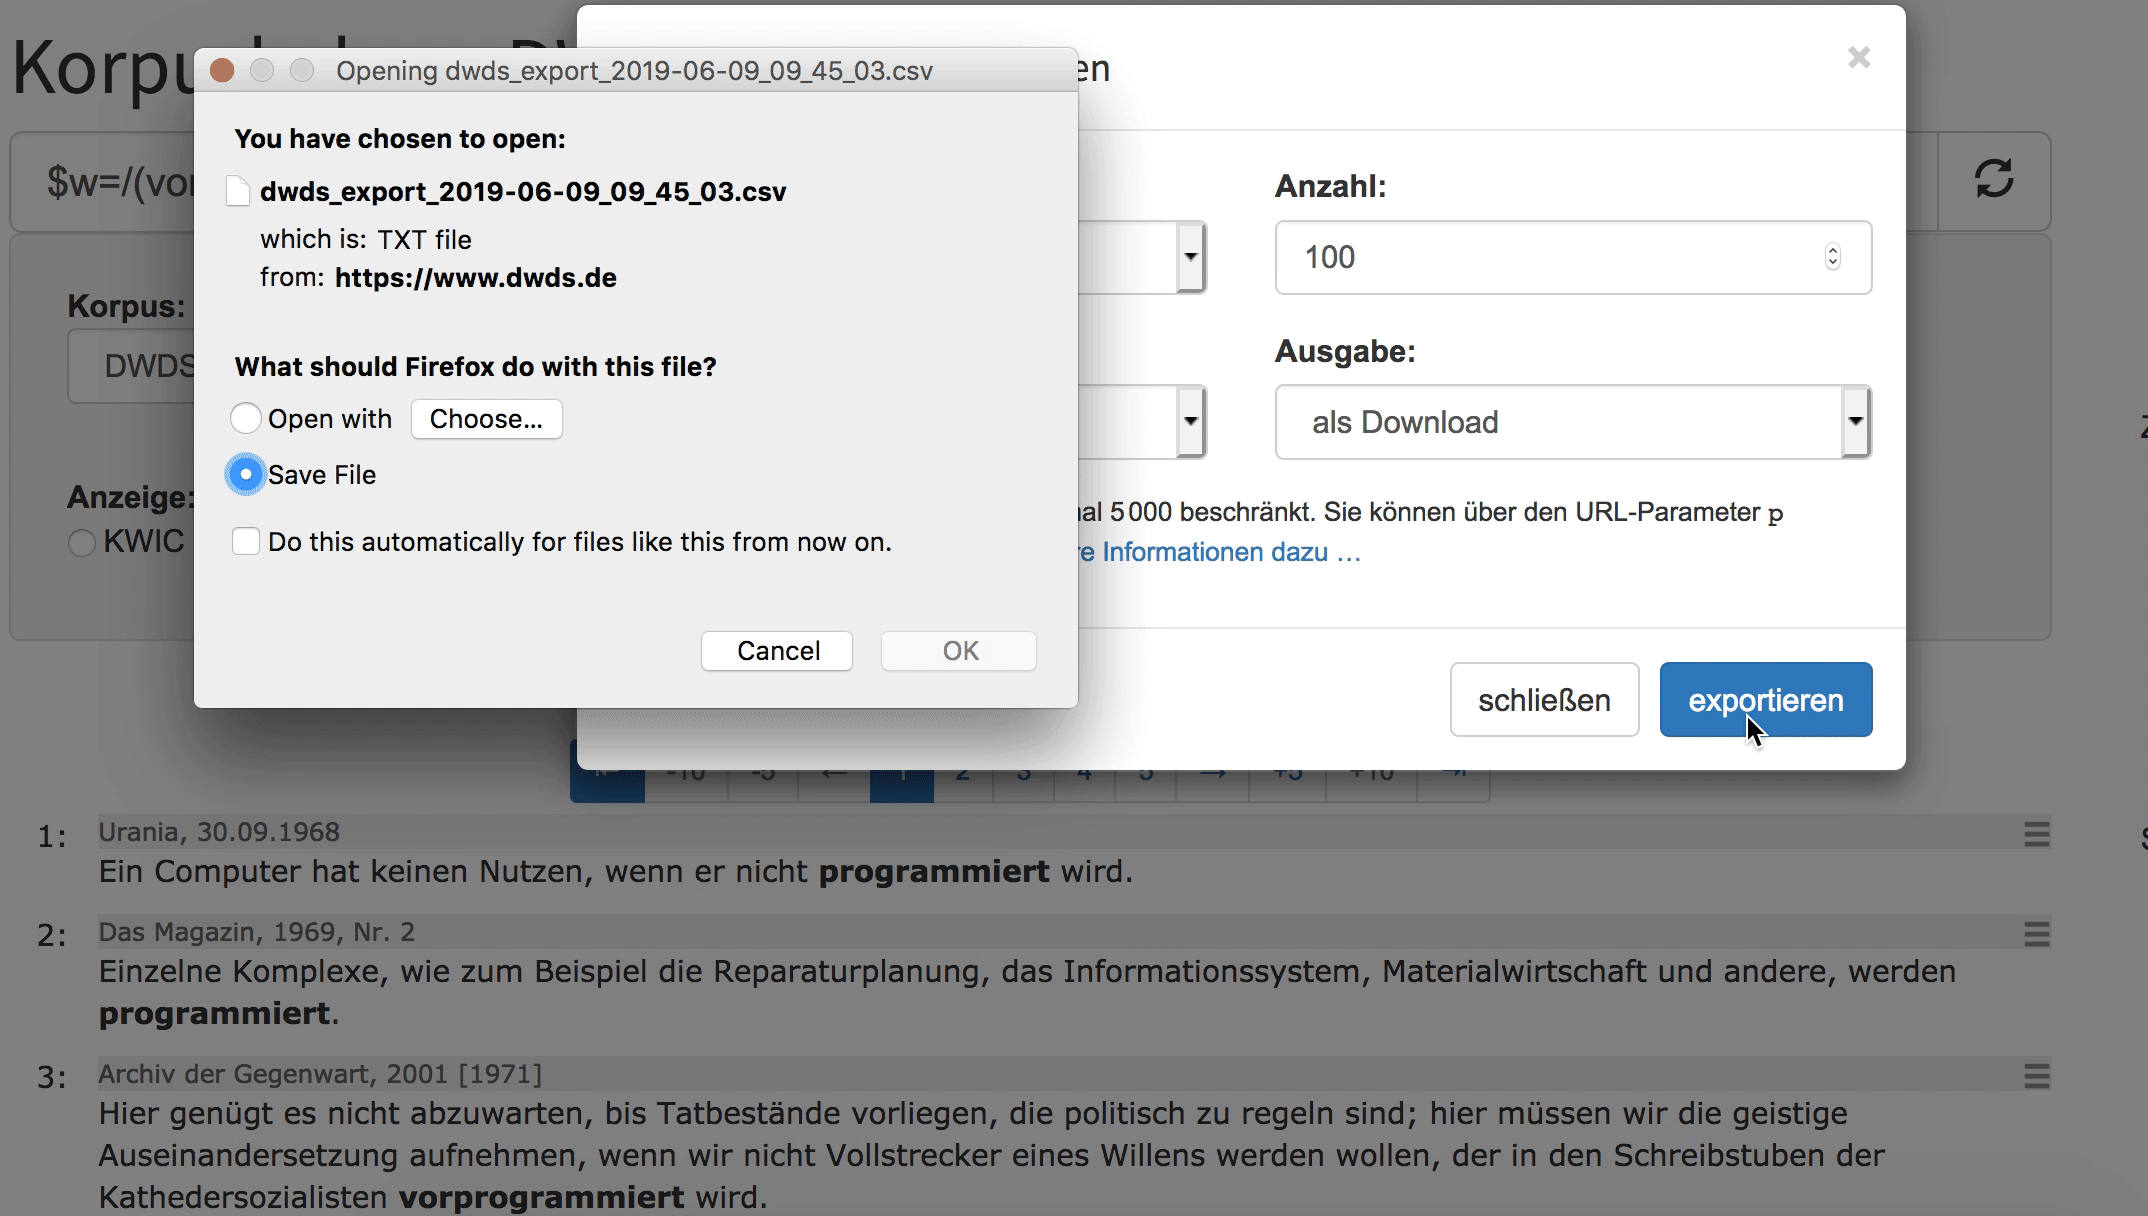
\includegraphics[width=5.37in]{docs/fig/dwdsdownload} \caption{Export aus dem DWDS}\label{fig:dwdsexp}
\end{figure}

Eine solche Sammlung von Korpusbelegen, wie wir sie jetzt exportiert
haben, nennt man in der Korpuslinguistik \textbf{Konkordanz}. Der
Formatname \enquote{CSV} steht für \enquote{Comma-Separated Values}. Das
heißt, in der Datei sind die einzelnen Werte durch Kommata voneinander
abgetrennt. In einem Texteditor sieht das Ganze so aus wie in
\ref{fig:dwdseditor}. Wie Sie sehen, enthält die Datei neben den
Korpusbelegen selbst auch Metadaten zu den einzelnen Belegen, z.B. zu
Autor*in, Titel etc.

\begin{figure}
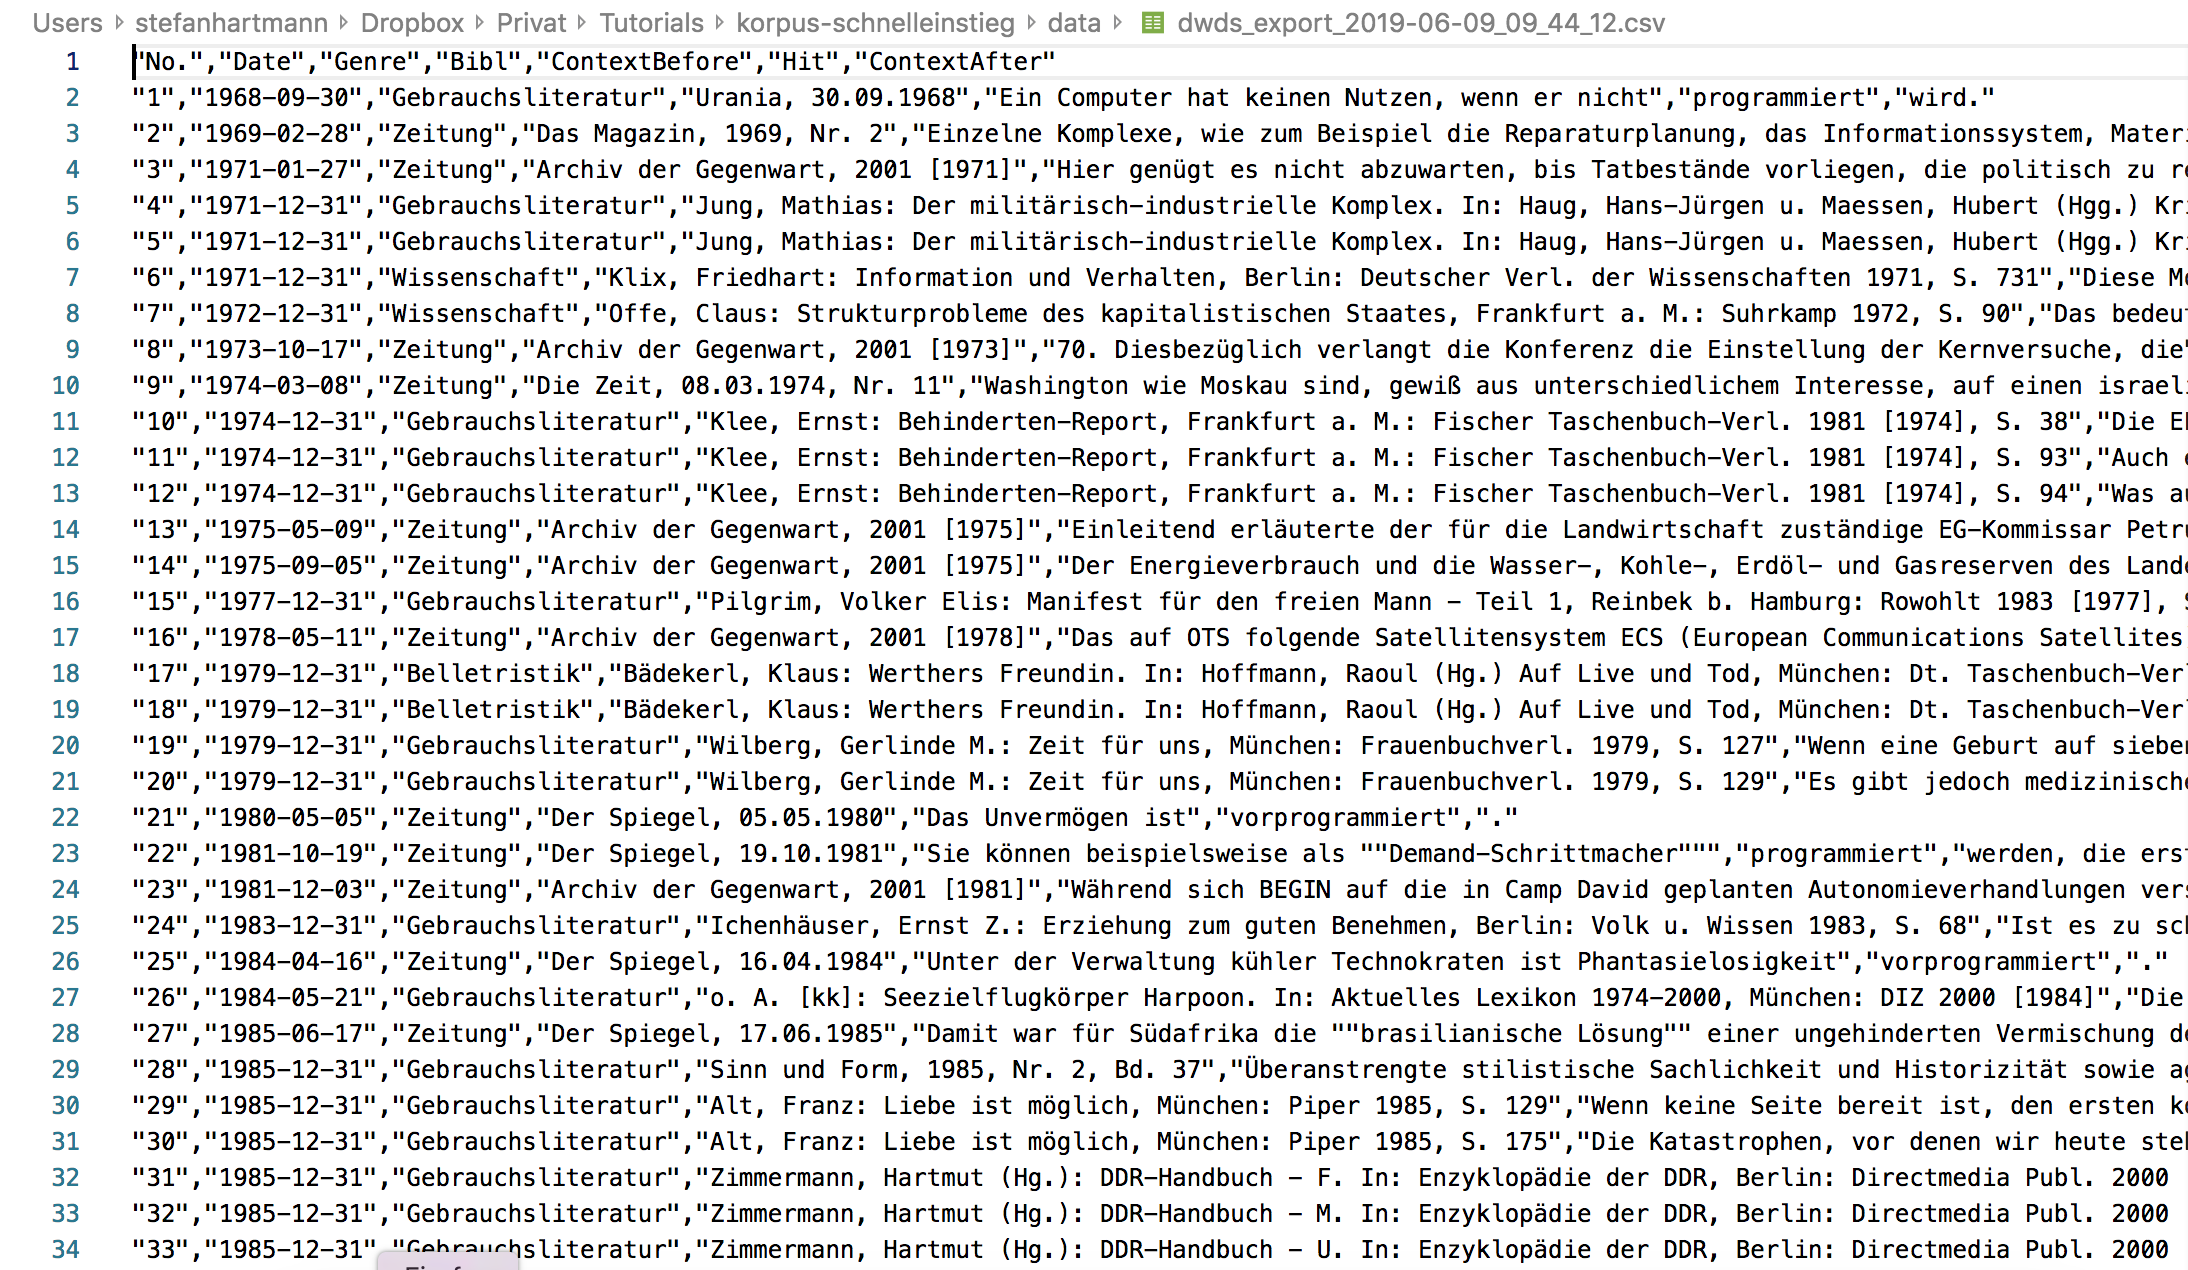
\includegraphics[width=4.86in]{docs/fig/conc_in_editor} \caption{Konkordanz im Texteditor}\label{fig:dwdseditor}
\end{figure}

Damit können wir zunächst noch wenig anfangen: Wir wollen die Konkordanz
in ein Tabellenkalkulationsprogramm einlesen.

\subsubsection{Import in ein
Tabellenkalkulationsprogramm}\label{import-in-ein-tabellenkalkulationsprogramm}

Wenn Sie Microsoft Excel auf Ihrem Rechner installiert haben, sind die
Default-Einstellungen höchstwahrscheinlich so gesetzt, dass CSV-Dateien
in Excel geöffnet werden, wenn Sie darauf doppelklicken. Warum das keine
gute Idee ist, zeigt der folgende Screenshot \ref{fig:excel1} (rote
Hervorhebungen von mir nachträglich hinzugefügt).

\begin{figure}
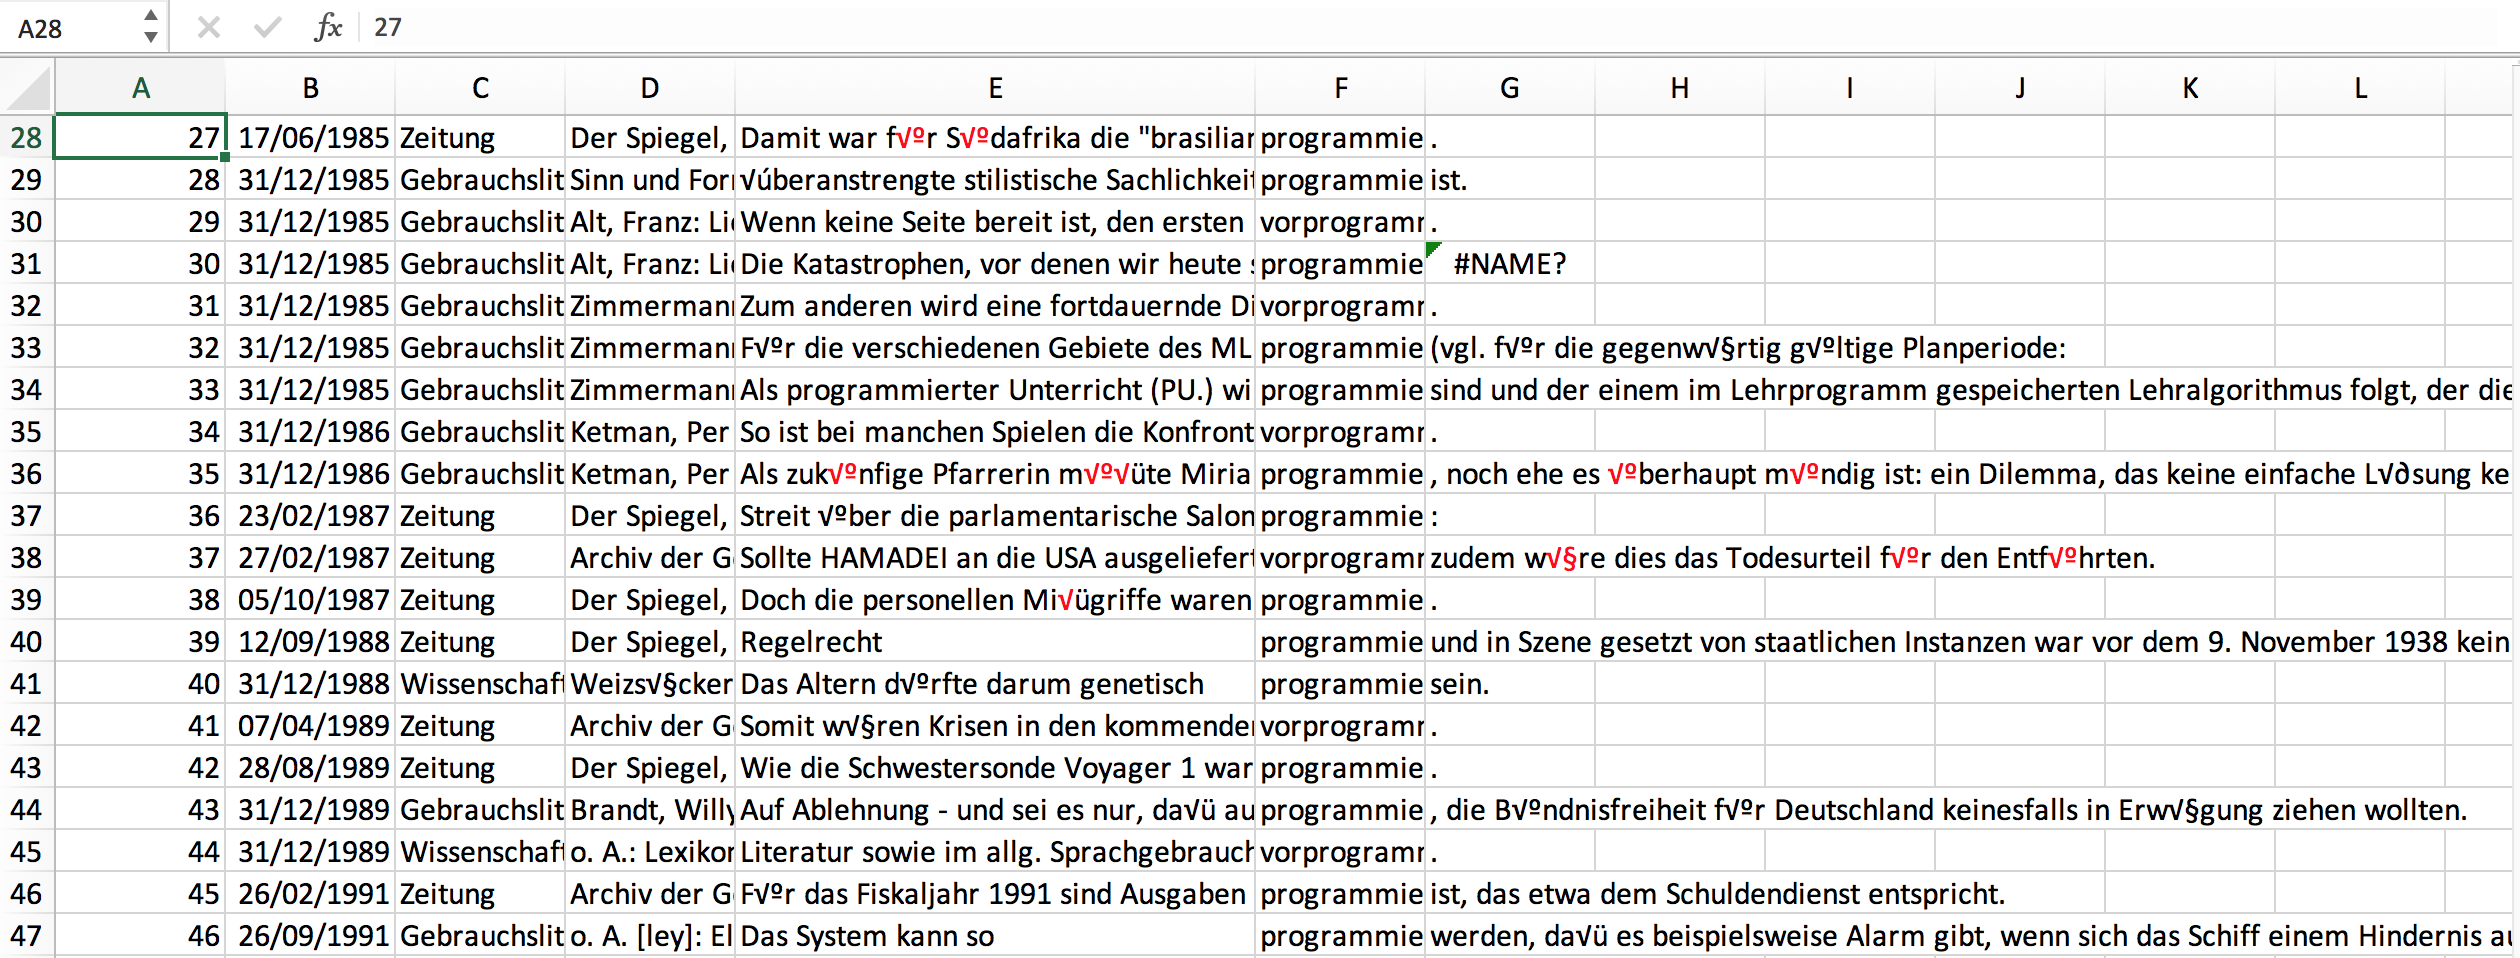
\includegraphics[width=5.04in]{docs/fig/conc_in_excel_bad} \caption{Konkordanz bei direktem Öffnen in Excel}\label{fig:excel1}
\end{figure}

Hier sind einige Sonderzeichen verlorengegangen, weil Excel die
Kodierung der Datei nicht richtig erkannt hat. Es gibt mehrere Wege,
diesem Problem zu begegnen. Ich empfehle hier zwei: Einen für
\protect\hyperlink{import-in-excel}{Excel} und einen für die freie
Alternative \protect\hyperlink{import-in-calc}{Calc}.

\hypertarget{import-in-excel}{\paragraph{Import in
Excel}\label{import-in-excel}}

\begin{enumerate}
\def\labelenumi{\arabic{enumi}.}
\item
  Öffnen Sie die Datei in einem Texteditor. Für Windows empfehle ich
  Notepad++, für Mac die kostenlose (und für unsere Zwecke völlig
  ausreichende) Version von BBEdit, für Linux gibt es z.B. Notepadqq.
\item
  Markieren Sie mit Strg+A bzw. Cmd+A den gesamten Text.
\item
  Öffnen Sie ein leeres Tabellenblatt in Excel. Die nächsten Schritte, 4
  bis 7, sind in \ref{fig:importexcel} visualisiert.
\item
  In den meisten Fällen sollten Sie nun einfach mit Strg+V bzw. Cmd+V
  die Daten einfügen könnn. In manchen Fällen müssen Sie jedoch, wie im
  Screencast \ref{fig:importexcel}, die Option \enquote{Paste Special}
  verwenden (dt. \enquote{Inhalte einfügen}) und angeben, dass Sie den
  Unicode-Text einfügen möchten.
\item
  Mit Klick auf das kleine Klemmbrett-Symbol gelangen Sie zum
  Textimport-Assistenten. Hier müssen Sie Excel sagen, wie der
  eingefügte Text strukturiert ist. Auf der ersten Seite sagen Sie, dass
  es sich um einen Text handelt, bei dem die einzelnen Spalten durch ein
  Trennzeichen getrennt sind (\enquote{Delimited}) -- diese Option ist
  in der Regel schon angewählt. Außerdem teilen Sie Excel hier mit, dass
  der eingefügte Text UTF-8-formatiert ist.
\item
  Auf der nächste Seite des Textimport-Assistenten geben Sie an, dass
  Kommata als Spaltentrenner benutzt werden. Bei den Textqualifizierern
  müssen Sie nichts ändern, da hier schon Anführungszeichen ausgewählt
  sind: Wie Sie in \ref{fig:dwdseditor} sehen können, werden
  Anführungszeichen in der CSV-Datei genutzt, um zusammengehörigen Text
  zusammenzuhalten (denn wären sie nicht da, würde Excel jedes Komma im
  Text für einen Spaltentrenner halten)
\item
  Dieser letzte Schritt erübrigt sich meistens, kann aber nicht schaden:
  Zuletzt können Sie noch alle Spalten als \enquote{Text} formatieren.
  (Die Datumsspalte können Sie prinzipiell auch als \enquote{Datum}
  formatieren, falls Sie ausschließlich in Excel weiterarbeiten, aber
  tendenziell rate ich davon ab -- gerade bei einer späteren Konversion
  in andere Dateiformate kann dabei alles mögliche schiefgehen\ldots{})
  Tipp: Um alle Spalten auf einmal als \enquote{Text} zu formatieren,
  einfach im Fenster ganz nach rechts scrollen und mit gedrückter
  Shift-Taste auf die letzte Spalte klicken, dann sind alle Spalten
  markiert.
\end{enumerate}

\begin{figure}
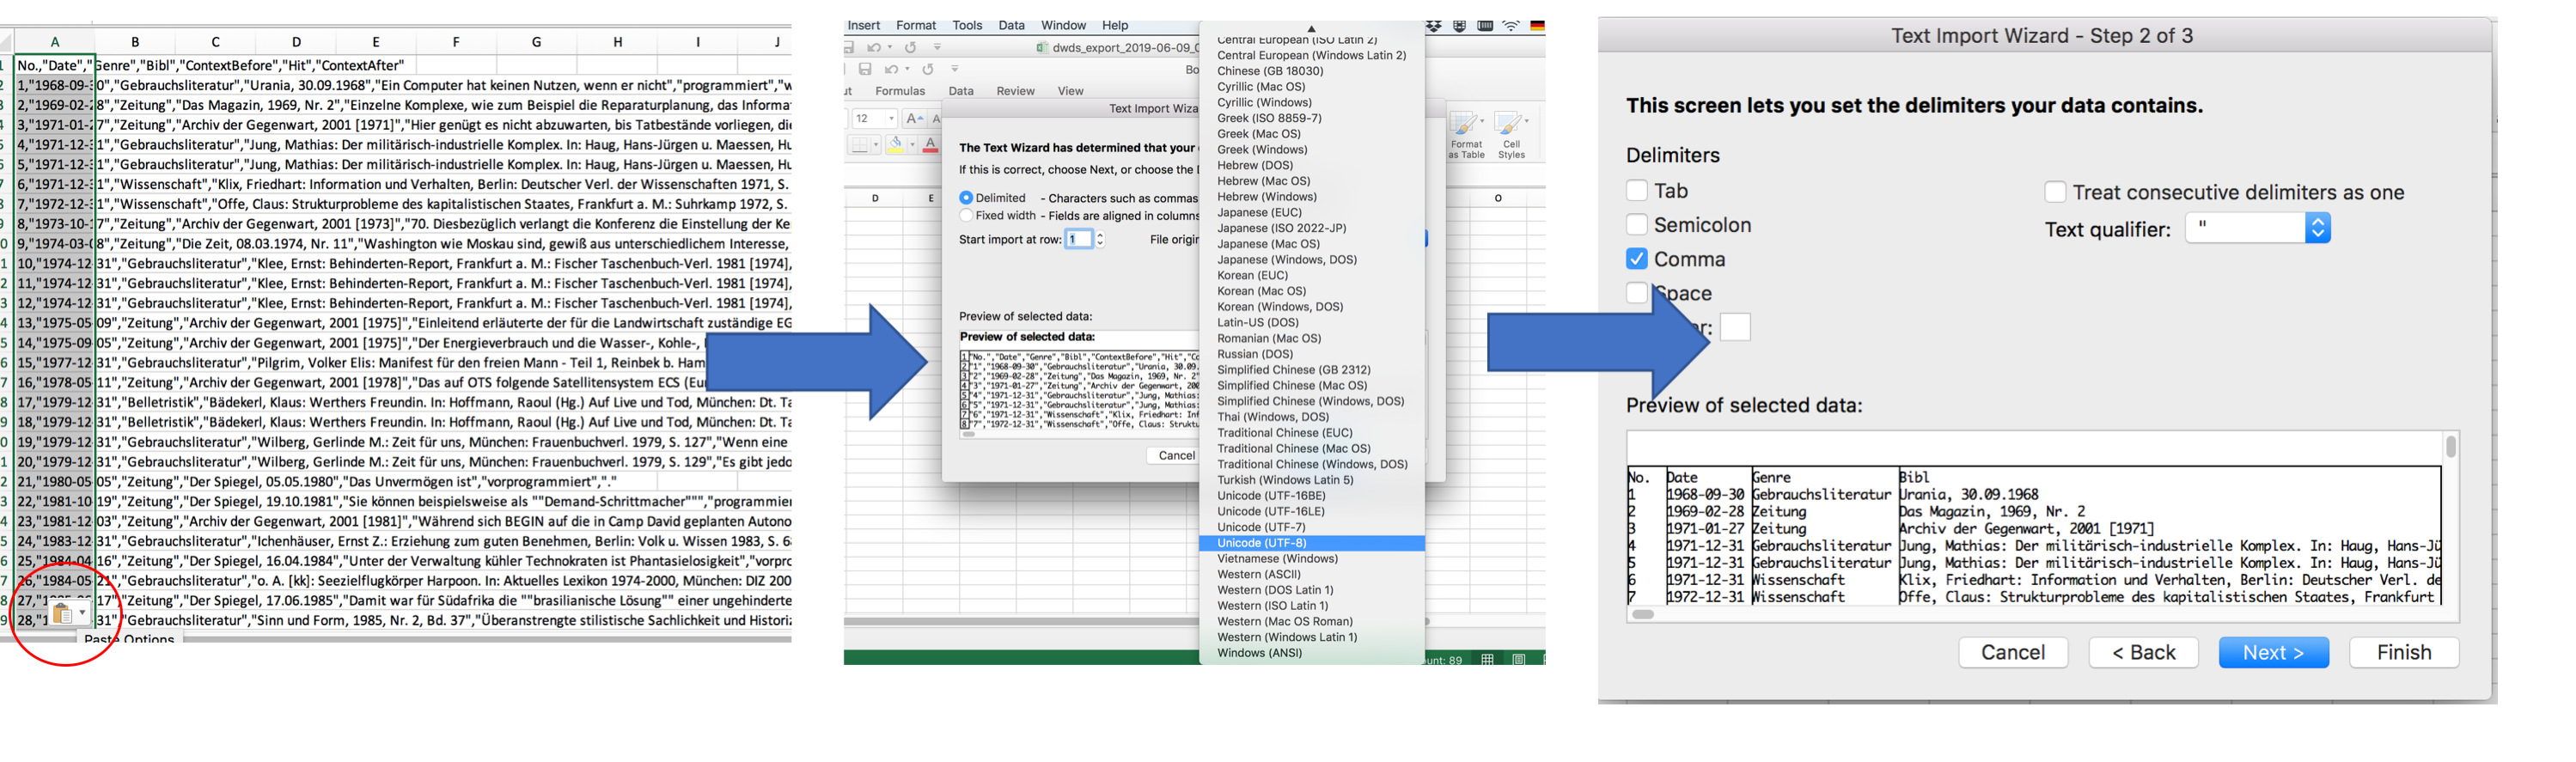
\includegraphics[width=6.66in]{docs/fig/import_in_excel} \caption{Import in Excel}\label{fig:importexcel}
\end{figure}

\hypertarget{import-in-calc}{\paragraph{Import in
Calc}\label{import-in-calc}}

Öffnet man die Datei im kostenlosen Tabellenkalkulationsprogramm Calc
von LibreOffice (mit Rechtsklick \textgreater{} Öffen mit), so öffnet
sich zunächst automatisch der Textimportassistent. Hier muss man Calc
mitteilen, welches Format die Datei hat. In unserem Fall ist der Text
UTF-8-kodiert, wir haben Kommas als Spaltentrenner und Anführungszeichen
als Textqualifizieren, wie in \ref{fig:calcimport}.

\begin{figure}
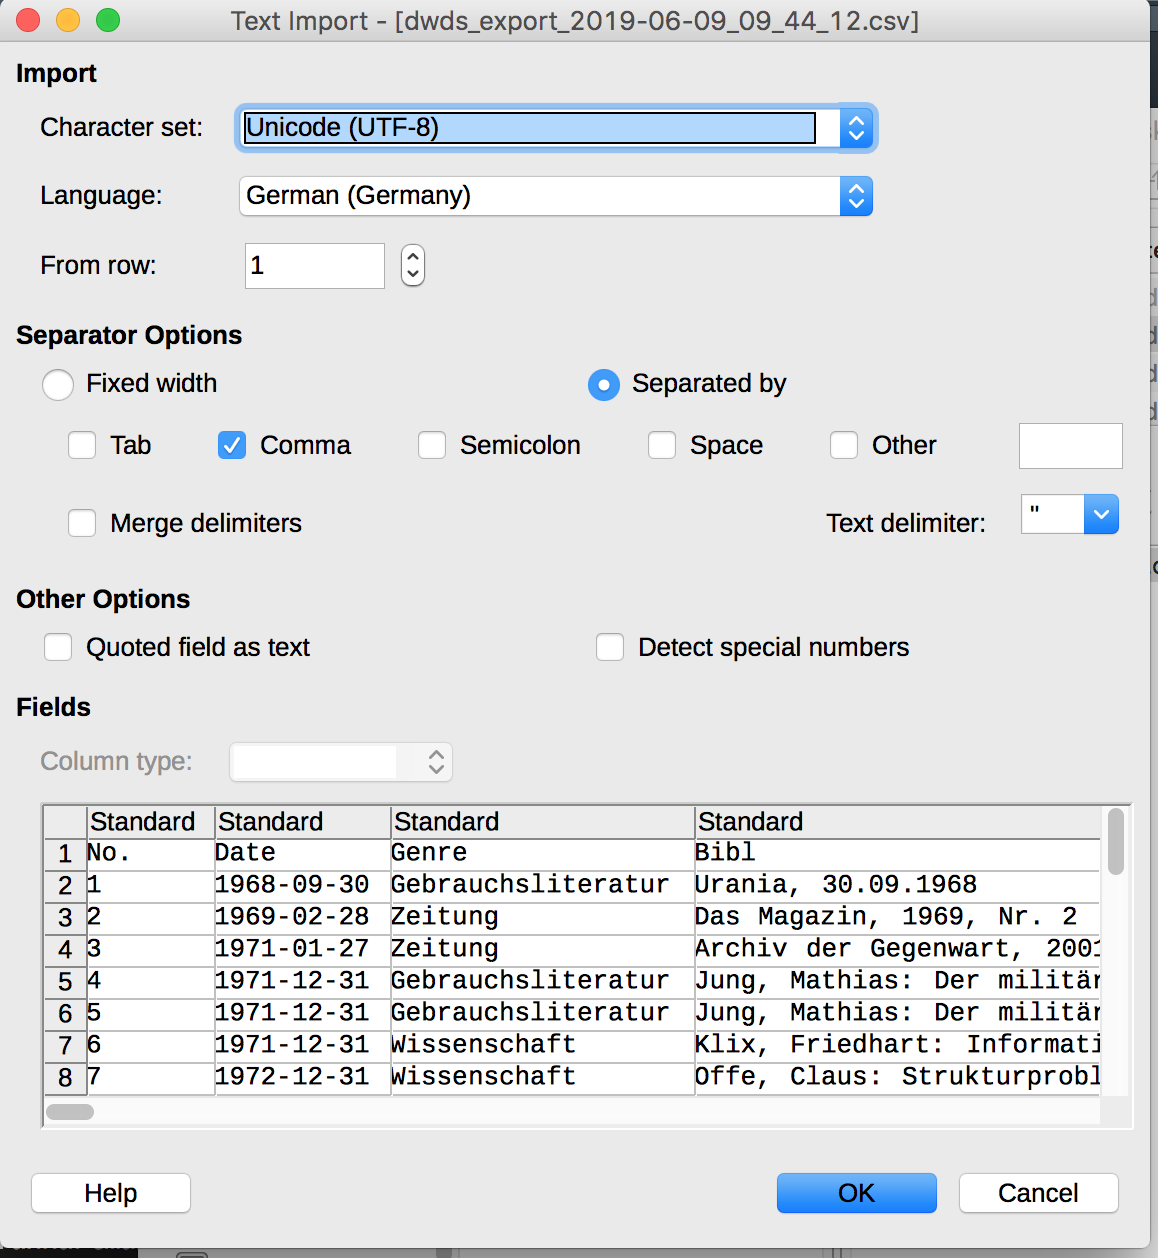
\includegraphics[width=0.5\linewidth,height=0.5\textheight]{docs/fig/calc_import} \caption{Import in Calc}\label{fig:calcimport}
\end{figure}

\section{Von der Konkordanz zur
Analyse}\label{von-der-konkordanz-zur-analyse}

Nun haben wir die Konkordanz erfolgreich in ein
Tabellenkalkulationsprogramm importiert. Hier können wir beliebig viele
weitere Spalten hinzufügen. Das können wir nutzen, um die exportierten
Belege mit \textbf{Annotationen} zu versehen.

\subsection{Annotation}\label{annotation}

Versieht man Daten mit zusätzlichen Informationen, so nennt man diesen
Prozess Annotation. In der Korpuslinguistik stellt die Annotation einen
ganz wesentlichen Schritt dar, der gewissermaßen die Brücke schlägt von
der qualitativ-philologischen Analyse einzelner Belege zur quantitativen
Auswertung.

Wir nutzen im Folgenden die Annotation, um unsere Daten in Kategorien zu
unterteilen, die für unsere Fragestellung sinnvoll sind. Dafür müssen
wir uns zunächst darüber im Klaren sein, was wir von unseren Daten
überhaupt wissen wollen, d.h. wir müssen unsere eingangs genannte
Fragestellung operationalisieren.

Zur Erinnerung: Unsere Fragestellung lautet, ob bei prädikativem
Gebrauch \emph{vorprogrammiert} gegenüber \emph{programmiert} bevorzugt
wird, wenn es sich um einen metaphorischen Kontext handelt.

Konkret bedeutet das, dass wir für jeden Datenpunkt folgende Fragen
beantworten müssen:

\begin{enumerate}
\def\labelenumi{\arabic{enumi}.}
\item
  Handelt es sich um eine prädikative Verwendung? -- Schon ein kurzer
  Blick auf die Daten zeigt, dass sich notwendigerweise einige
  \textbf{Fehltreffer} eingeschlichen haben: Häufig finden sich z.B.
  Passivkonstruktionen wie \emph{Es gibt jedoch medizinische Gründe, aus
  denen eine Geburt eingeleitet oder sogar programmiert werden muß}. Uns
  interessieren aber nur Fälle, in denen das Partizip selbst das
  Prädikat bildet, also z.B. \emph{Der Computer ist programmiert} und
  \emph{Die Katastrophe war vorprogrammiert}.
\item
  Handelt es sich um eine metaphorische Verwendung? -- Während
  beispielsweise Computer oder Roboter im wörtlichen Sinne programmiert
  werden, bezieht sich der Begriff bei Krisen und Katastrophen darauf,
  dass Voraussetzungen geschaffen wurden, die unausweichlich den
  thematisierten unschönen Ausgang zur Folge haben. Es liegt also ein
  metaphorischer Gebrauch vor, bei der Aspekte der Quelldomäne
  \enquote{Technik} auf eine abstraktere Zieldomäne übertragen werden.
\end{enumerate}

In den nächsten Abschnitten wollen wir uns beiden Fragen etwas genauer
zuwenden.

\subsubsection{Annotation prädikativ
vs.~nicht-prädikativ}\label{annotation-pradikativ-vs.nicht-pradikativ}

Wenn wir Daten annotieren, besteht eine wesentliche Herausforderung
immer in der \textbf{Operationalisierung} konkreter Fragestellungen. In
vielen Fällen ist es so, dass wir die Frage, die uns interessiert, auf
den ersten Blick für jeden Datenpunkt klar beantworten zu können
glauben. Bei genauerem Hinsehen ergeben sich dann aber doch einige
Zweifelsfälle. So ist es auch hier: Um die Frage operationalisieren zu
können, muss man zunächst einmal die Entscheidung treffen, ob man eine
Struktur wie \emph{Der Computer ist programmiert} als Zustandspassiv mit
\emph{sein} als Hilfsverb (analog zum Vorgangspassiv mit \emph{werden}
als Hilfsverb) oder als Konstruktion aus der Kopula \emph{sein} und dem
Partizip II \emph{programmiert} interpretiert. Wir entscheiden uns hier
für Letzteres. Jedoch zeigt dieses Beispiel: Wie wir Daten
interpretieren, hängt oft genug von unserem theoretischen Zugang ab. Das
ist nicht weiter schlimm, sondern liegt in der Natur der Sache --
Wissenschaft kann nie ganz frei von Theorie und nie ganz frei von
Interpretation sein. Wichtig ist, dass die Entscheidung, die wir
treffen, sich gut begründen lässt und konsequent durchgehalten wird.

Wie setzen wir die Annotation nun in unserer Tabelle um? Auch hier zeige
ich wieder Wege für \protect\hyperlink{umsetzung-in-excel}{Excel} und
\protect\hyperlink{umsetzung-in-calc}{Calc}. Gerade die unten skizzierte
Möglichkeit, Daten als \enquote{Tabelle} zu formatieren, finde ich
persönlich an Excel sehr hilfreich, weshalb ich Excel i.d.R. bevorzuge.
Allerdings halte ich es auch für wichtig, sich in der Wissenschaft nicht
von proprietärer Software oder proprietären Datenformaten abhängig zu
machen, und nicht jede Uni hat eine Office-Lizenz -- deshalb zeige ich
auch den Weg mit der freien Alternative auf.

\hypertarget{umsetzung-in-excel}{\paragraph{Umsetzung in
Excel}\label{umsetzung-in-excel}}

Zunächst empfiehlt es sich, die Tabelle im Excel-Standardformat .xlsx zu
speichern.

Excel bietet die schöne Möglichkeit, Daten als Tabelle zu formatieren.
Das ist über den Reiter Einfügen \textgreater{} Tabelle möglich, wie in
\ref{fig:excelastable} gezeigt. In der Regel erkennt Excel automatisch
die Dimensionen der Tabelle, sodass Sie nur noch anklicken müssen, dass
die Tabelle Überschriften hat, und dann auf \enquote{OK} klicken können,
und schon sind alle Zellen schön formatiert, und vor allem kann man über
die kleinen Pfeilsymbole oben die einzelnen Spalten nach bestimmten
Werten filtern, was sich im weiteren Verlauf der Arbeit noch als
nützlich erweisen kann. (Letzteres erreicht man auch über Daten
\textgreater{} Filter, aber mit der Tabellen-Option wird das Ganze
optisch noch ein bisschen hübscher, und vor allem muss man keinen neuen
Filter setzen, wenn man eine neue Spalte hinzufügt.)

Um die Belege im Kontext besser lesen zu können, empfiehlt es sich,
zunächst ein paar Feinjustierungen in der Formatierung vorzunehmen. So
können wir Spalten, die wir derzeit nicht benötigen (z.B. alle Spalten
mit Metadaten), zunächst ausblenden. (Nicht löschen! Im Zweifelsfall nie
Spalten löschen, wer weiß, wozu man sie später noch benötigt\ldots{})
Außerdem kann es hilfreich sein, den Text in der Spalte mit dem linken
Kontext rechtsbündig zu formatieren und die Breite der einzelnen Spalten
so anzupassen, dass man den Beleg und ausreichend viel Kontext lesen
kann und doch alle derzeit wichtigen Spalten gleichzeitig auf dem
Bildschirm zu sehen sind. Wenn Sie die HTML-Version dieses Dokuments
lesen, sehen Sie im weiteren Verlauf von Screencast
\ref{fig:excelastable} (nach der Formatierung der Daten als Tabelle),
wie eine solche Feinjustierung aussehen kann.

\begin{figure}
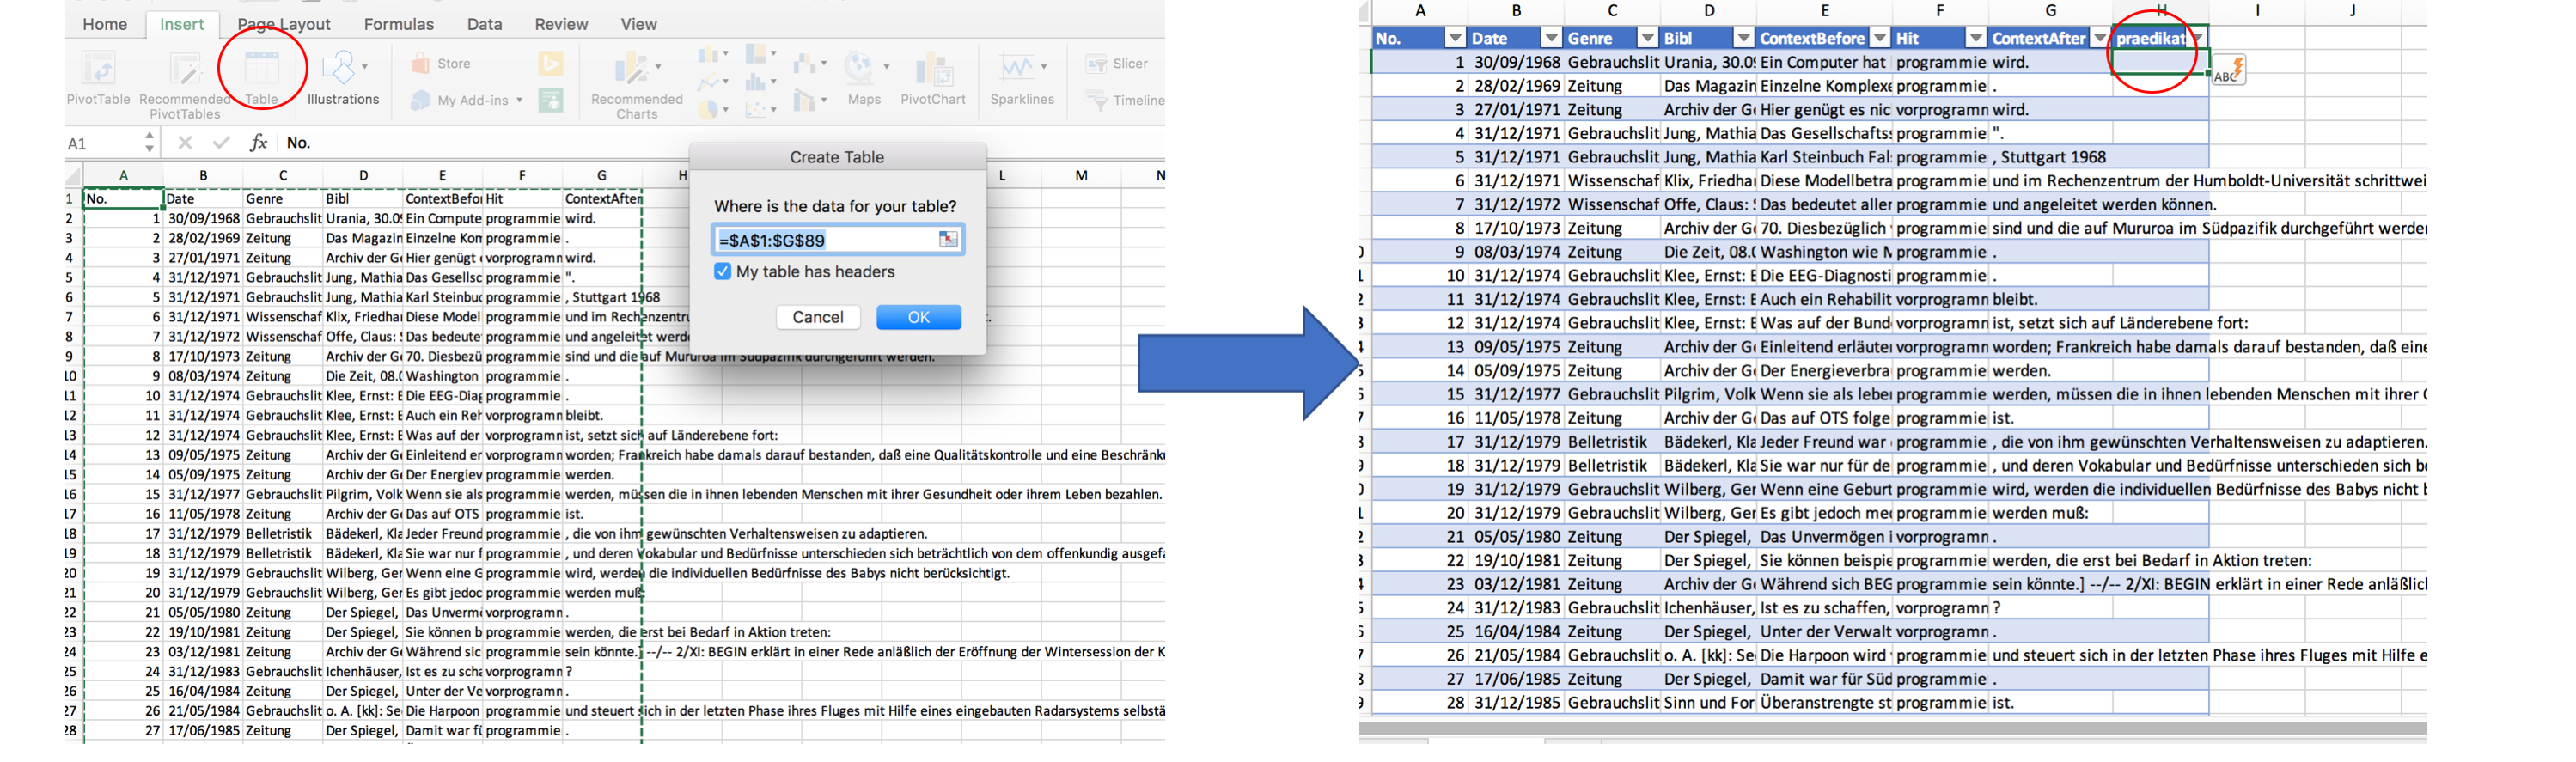
\includegraphics[width=6.66in]{docs/fig/excelastable01} \caption{Formatierung als Tabelle und Hinzufügen einer Annotationsspalte *praedikativ*}\label{fig:excelastable}
\end{figure}

 ‣ \textbf{Zeilenumbruch innerhalb von Tabellenspalten}

In einigen Fällen, in denen man sehr viel Text im linken und rechten
Kontext hat und in denen man für die Annotation auch auf den weiteren
Kontext angewiesen ist, kann es sinnvoll sein, die Tabelle so zu
formatieren, dass innerhalb der Zelle ein Zeilenumbruch vorgenommen
wird. Standardmäßig ist die Tabelle so formatiert, dass jede Zelle nur
eine Zeile hat, und was über die Zelle hinausgeht, wird nicht angezeigt
(ist aber trotzdem noch in den Daten vorhanden). Wenn man durch Klick
auf den Buchstaben oberhalb der Spalte, die man formatieren möchte,
zunächst die ganze Spalte markiert, kann man unter Rechtsklick
\textgreater{} Zellen formatieren im Tab \enquote{Alignment}
(\enquote{Ausrichtung}) die Option \enquote{Wrap text} (Zeilenumbruch)
aktivieren.

\begin{figure}
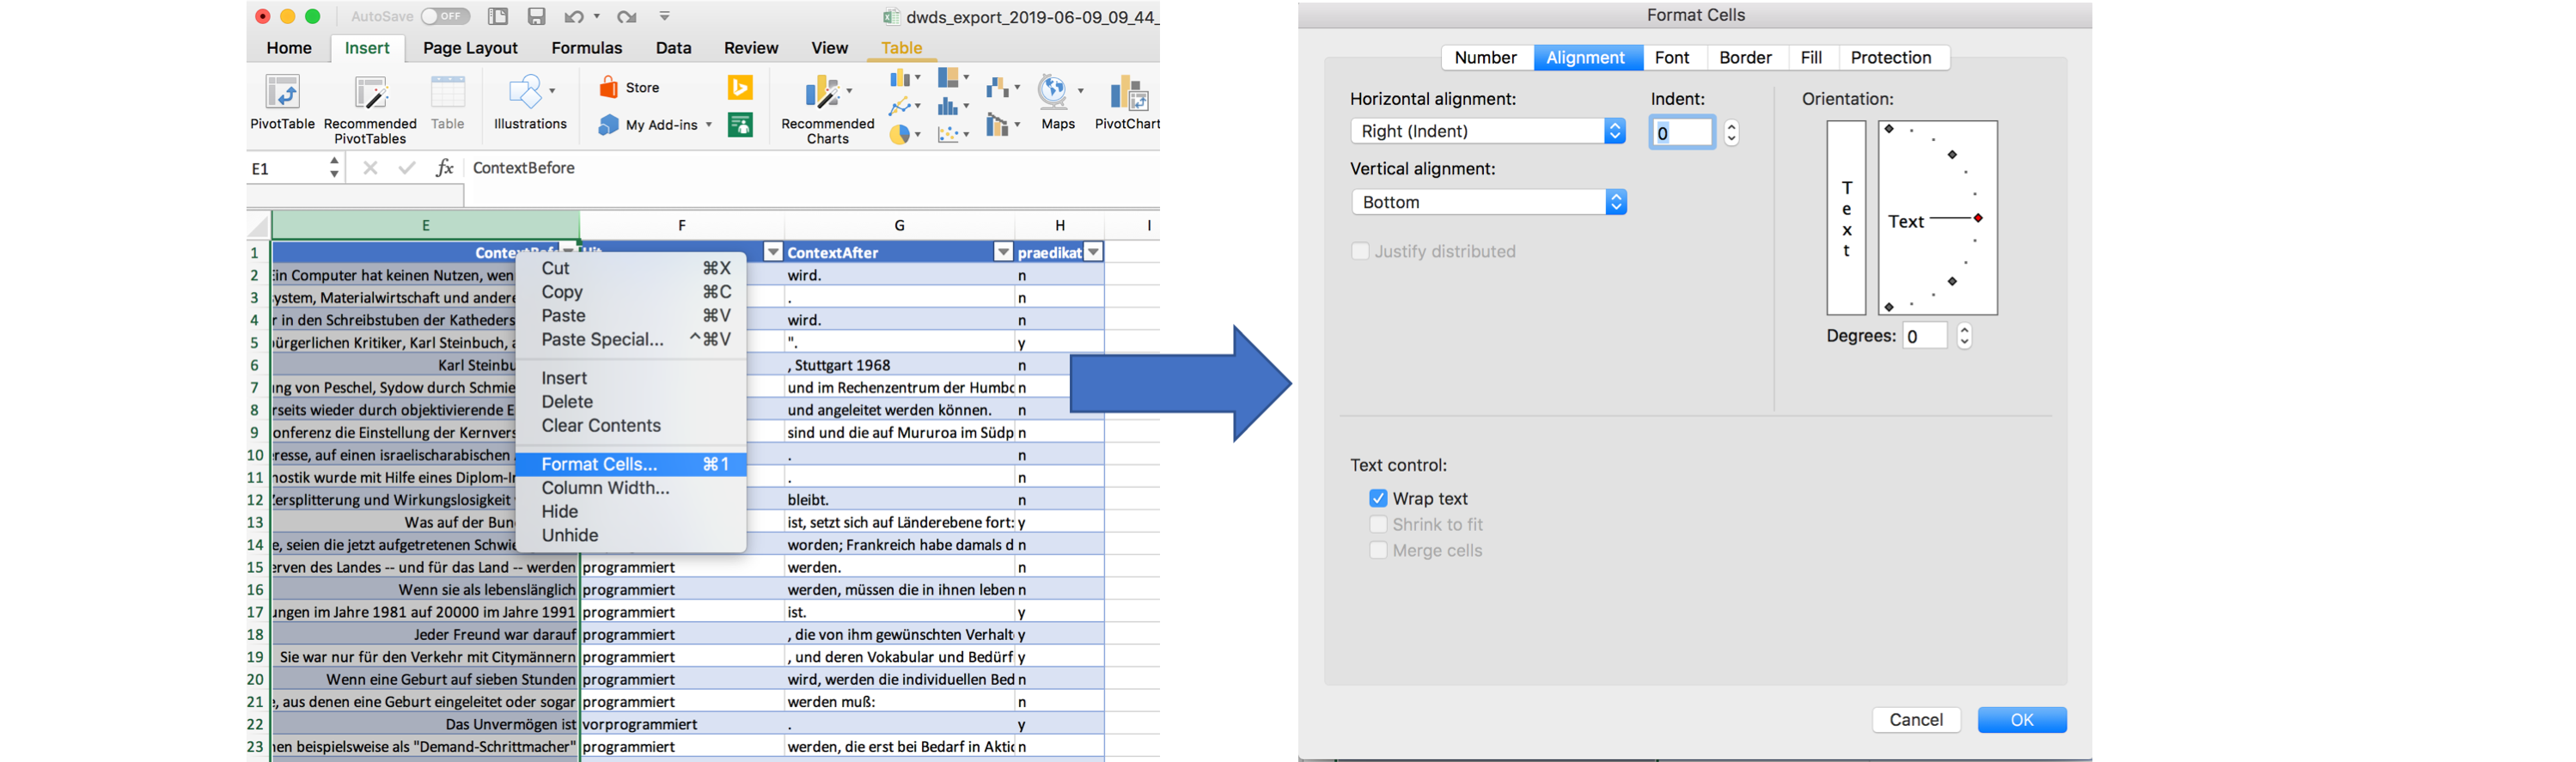
\includegraphics[width=6.66in]{docs/fig/excellinewrap} \caption{Zeilenumbruch innerhalb von Zellen einschalten}\label{fig:excelwrap}
\end{figure}

Als nächstes fügen wir eine neue Spalte rechts von der letzten
existierenden Spalte hinzu, der wir die Überschrift
\enquote{praedikativ} geben. (Wir könnten auch problemlos den Umlaut
verwenden, aber ich neige dazu, aus Vorsicht alle Sonderzeichen, die
Probleme bereiten könnten, wegzulassen.) Hier tragen wir nun für jeden
Datenpunkt ein, ob es sich um eine prädikative Verwendung handelt oder
nicht. Ich verwende hierfür gern die Werte \enquote{y} und \enquote{n},
weil sie schön kurz sind. j/n oder ja/nein gehen natürlich auch.

Um Zeit zu sparen, kann man auch nur einen der beiden Werte annotieren
und dann die leeren Zellen einfach auffüllen, wie in
\ref{fig:excelbulkchange} gezeigt: Hier sind die \enquote{y}-Werte schon
annotiert, alle anderen Zeilen sind leer. Nun filtert man erst die
\enquote{praedikativ}-Spalte so, dass nur noch die leeren Zellen zu
sehen sind, indem man die Zellen mit dem Wert \enquote{y} abwählt. Dann
markiert man die Spalte \enquote{praedikativ} von der ersten bis zur
letzten Zeile (die Überschrift wird nicht mitmarkiert). Gibt man nun
\enquote{n} ein (noch nicht Enter drücken!!), so erscheint der Wert
zunächst in der ersten Zeile. Drückt man nun statt der Eingabetaste
Strg+Enter (bzw. bei Mac Cmd+Enter), so wird der in der ersten Zeile
eingegebene Wert auf alle folgenden Zellen übertragen.

\begin{figure}
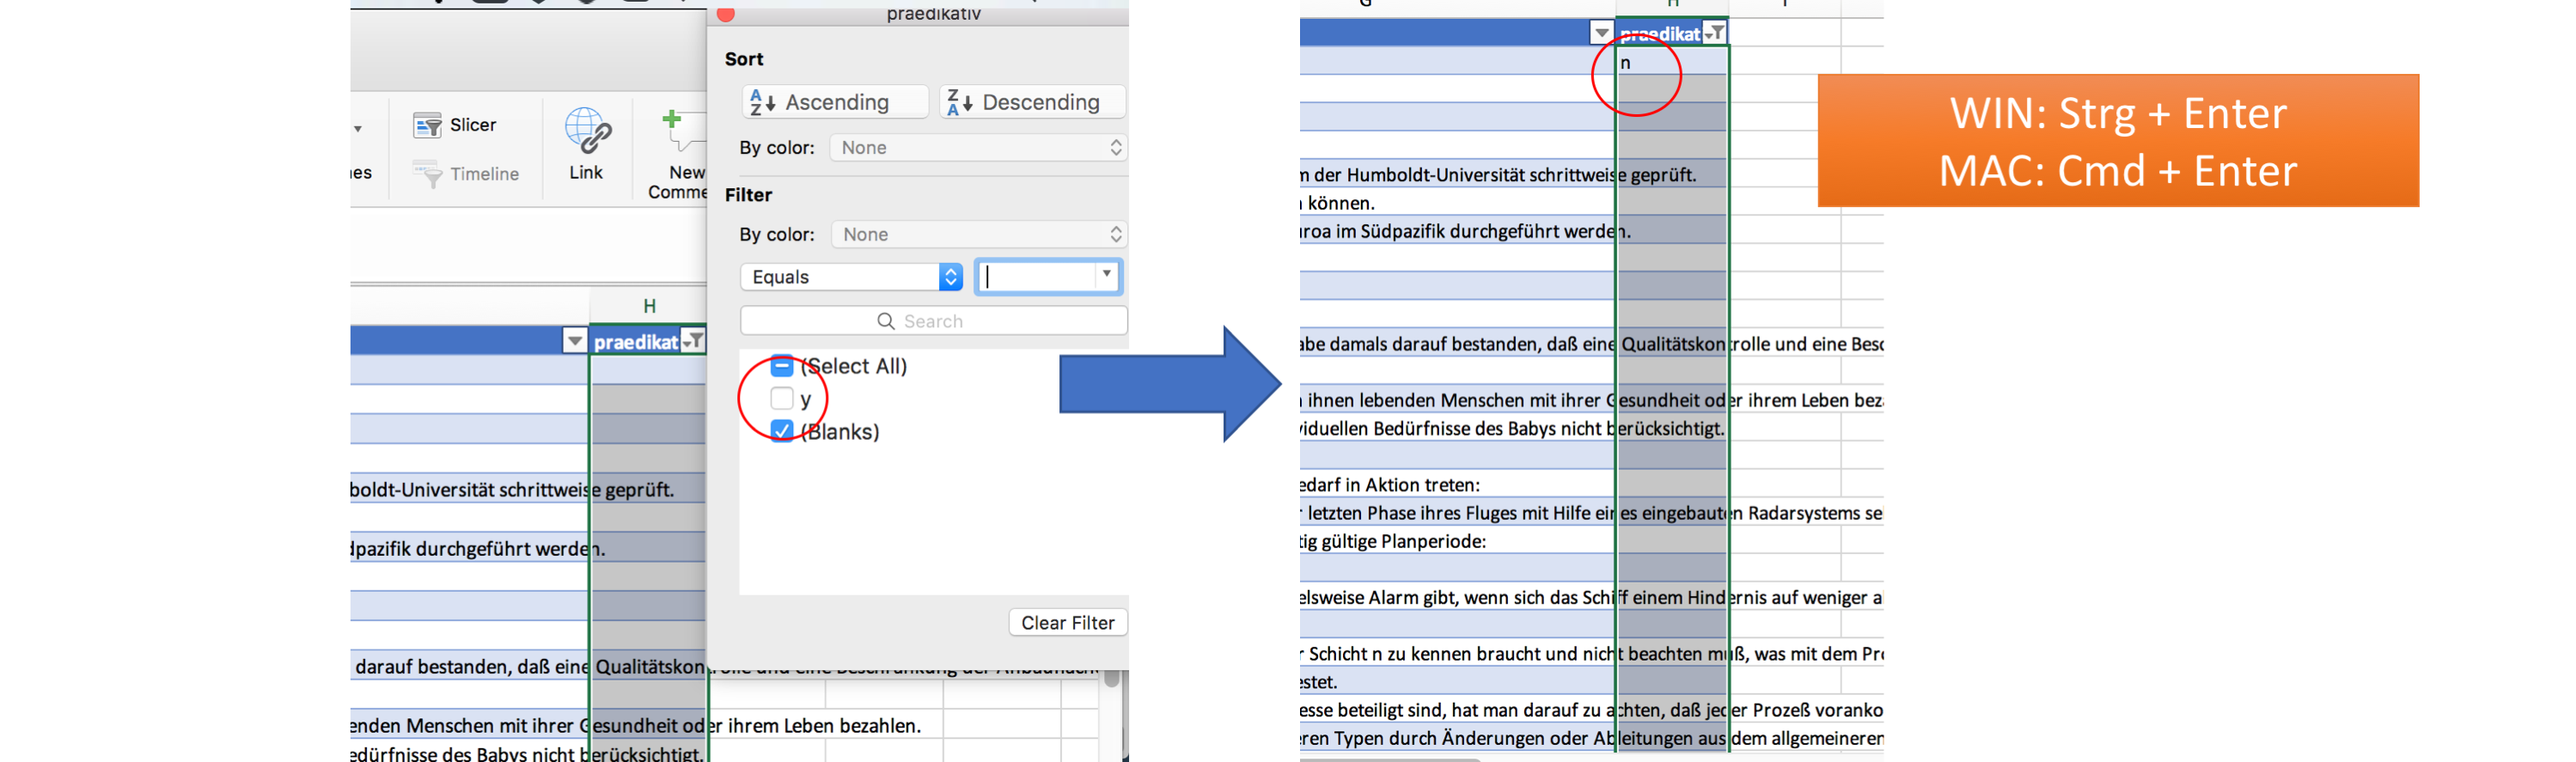
\includegraphics[width=6.66in]{docs/fig/excel_bulk_change} \caption{Eine Tabellenspalte wird so gefiltert, dass nur noch die leeren Zellen zu sehen sind, und allen leeren Zellen wird mit Strg/Cmd+Enter derselbe Wert zugewiesen.}\label{fig:excelbulkchange}
\end{figure}

Wenn wir nun den Filter herausnehmen, sehen wir, dass nun alle vorher
leeren Zeilen ein \enquote{n} haben, während alle Zeilen mit \enquote{y}
unverändert geblieben sind.

\hypertarget{umsetzung-in-calc}{\paragraph{Umsetzung in
Calc}\label{umsetzung-in-calc}}

In Calc empfiehlt es sich, zunächst einmal die Spaltenbreite anzupassen
und nicht benötigte Spalten auszublenden (nicht löschen -- im
Zweifelsfall niemals Spalten oder Zeilen löschen, wer weiß, wofür man
sie noch benötigt!). Ich selbst gehe in der Regel so vor, dass ich alle
Spalten bis auf diejenigen mit den eigentlichen Belegen (linker Kontext,
Treffer, rechter Kontext) ausblende und die Spalte mit dem linken
Kontext so formatiere, dass der Text rechtsbündig angezeigt wird. So
kann ich bequem den Beleg vom linken Kontext über den Treffer bis zum
Keyword lesen. In der HTML-Version dieses Tutorials sehen Sie das in
Screencast \ref{fig:calcformat}.

\begin{figure}
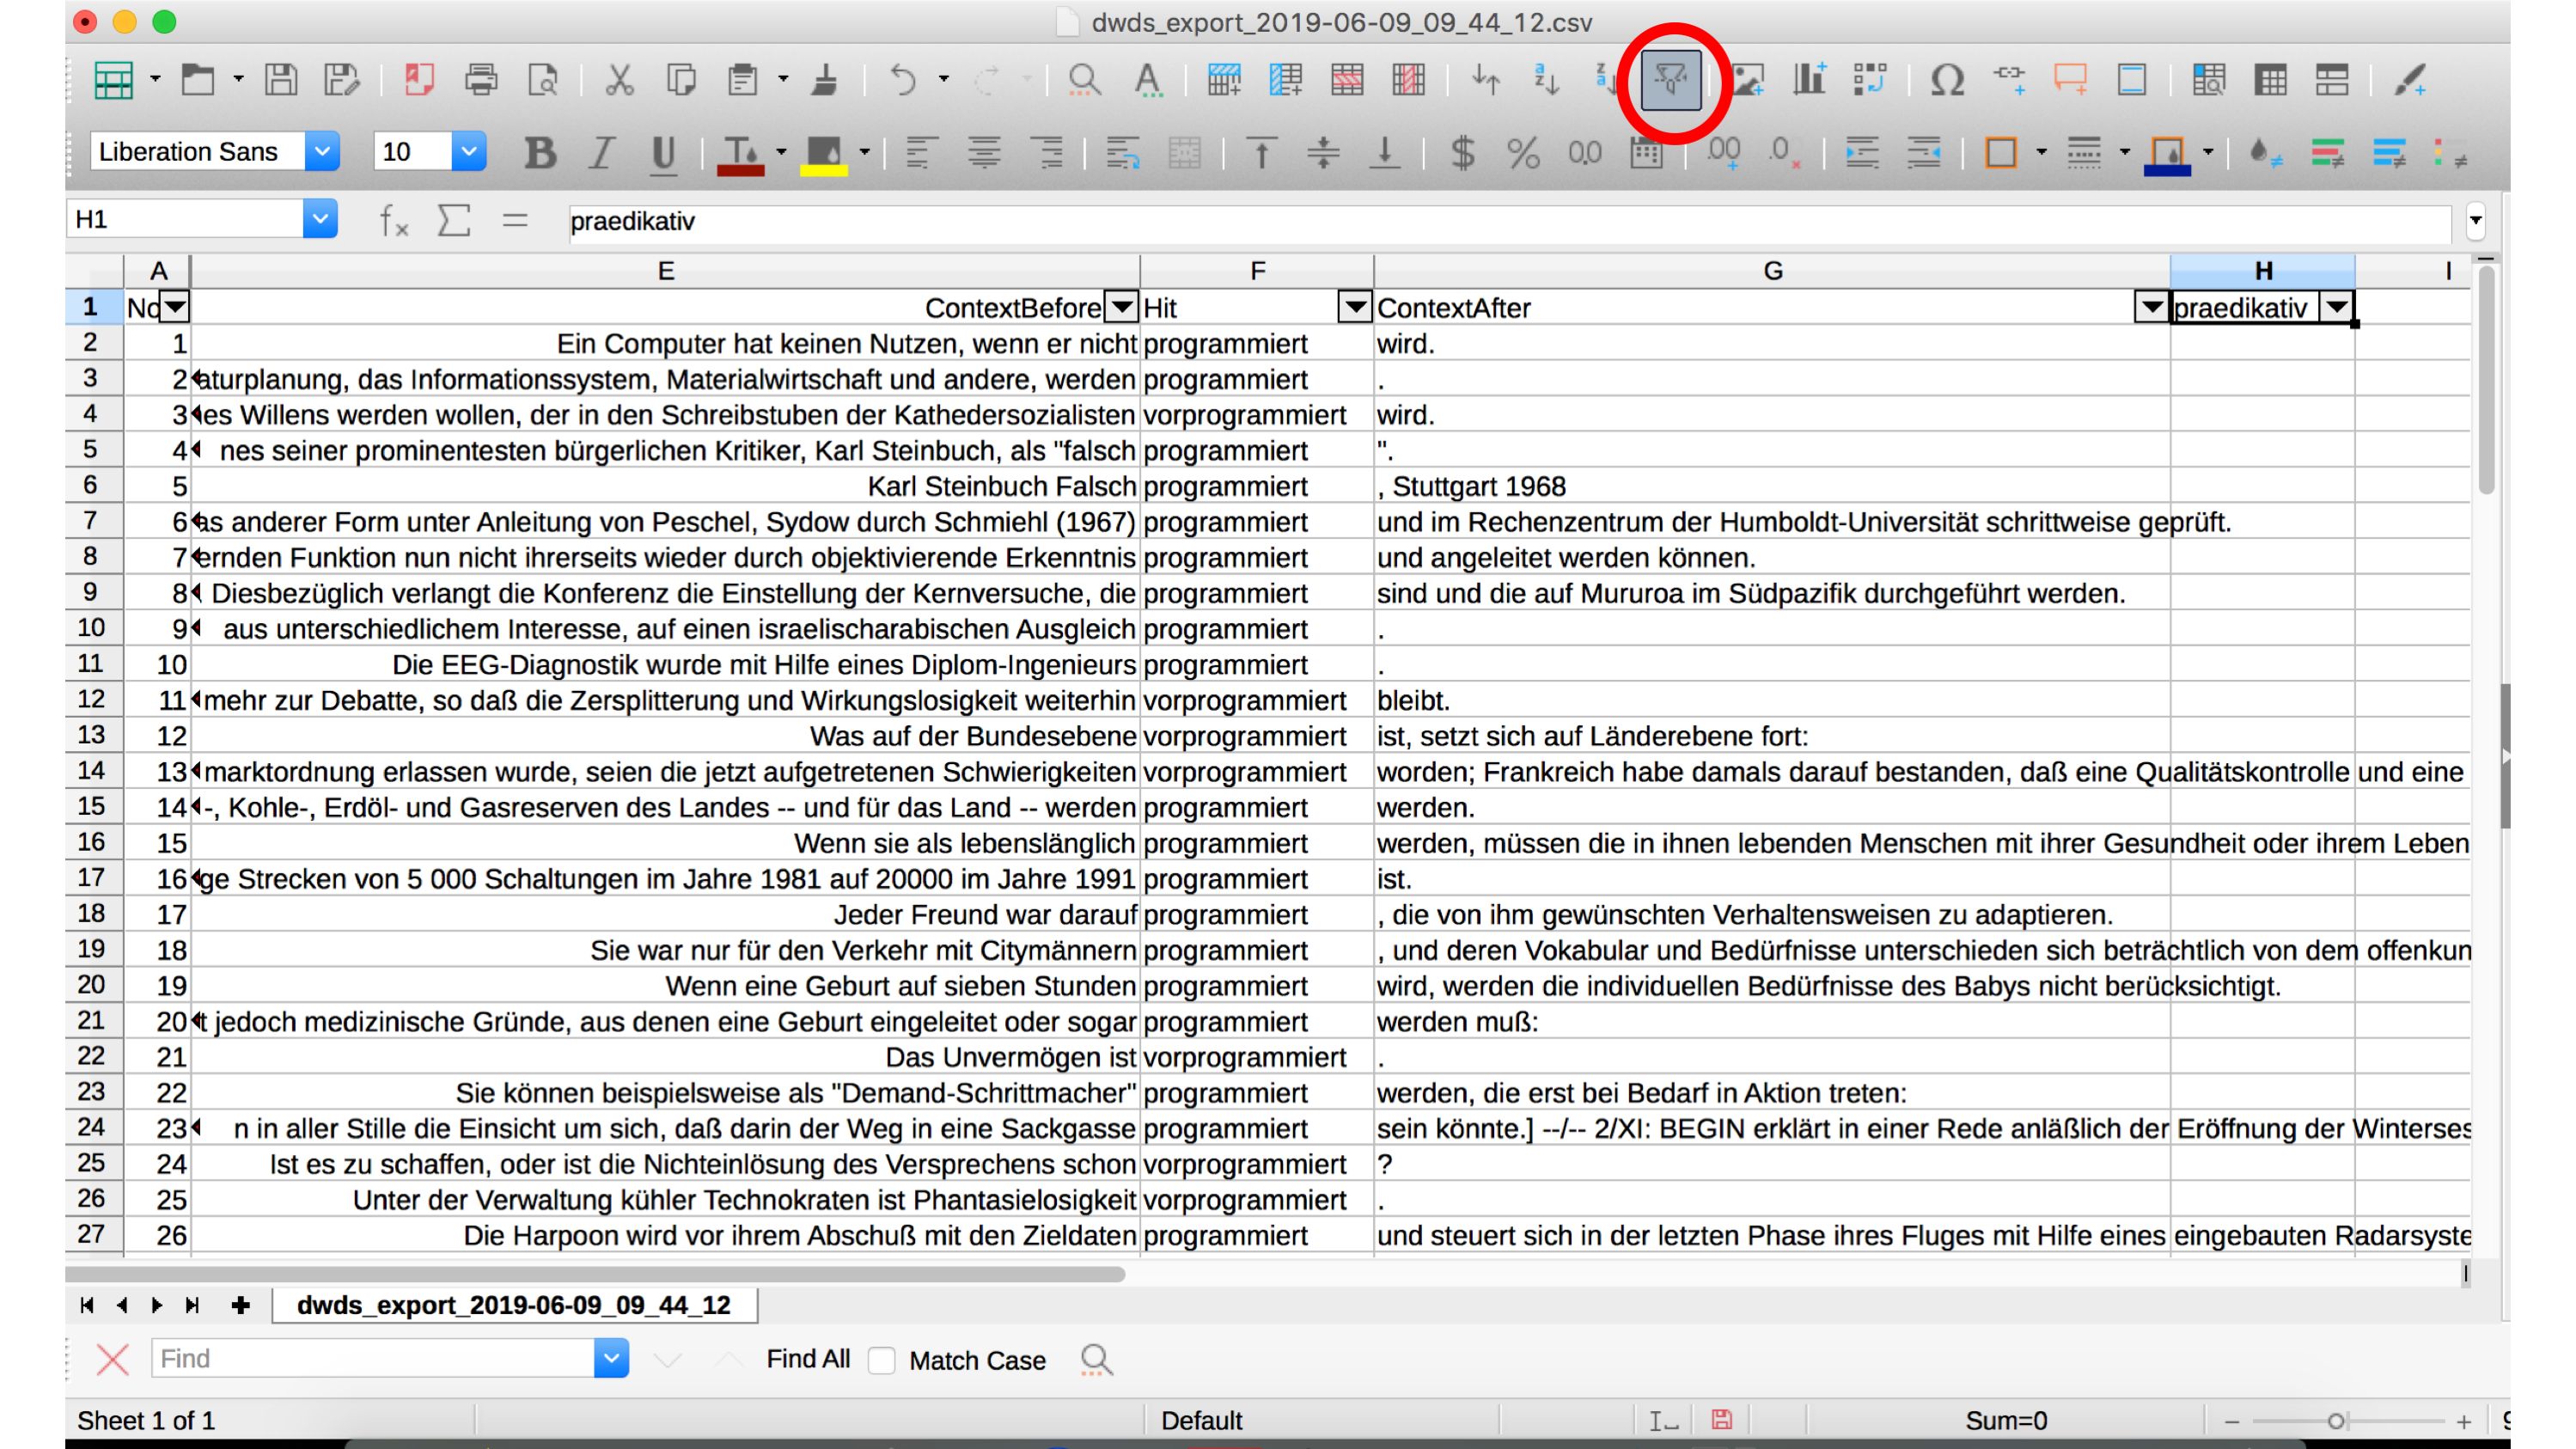
\includegraphics[width=6.66in]{docs/fig/calcformat} \caption{Formatierung der Tabelle in Calc und Setzen eines Filters}\label{fig:calcformat}
\end{figure}

Wenn Sie die Formatierungsoptionen für zukünftige Sitzungen speichern
möchten, müssen Sie die Datei in einem anderen Format, z.B. im
Calc-Standardformat .ods, speichern. Prinzipiell können Sie aber auch
einfach in der CSV-Datei weiterarbeiten. Wenn Sie die Datei
zwischenspeichern, werden dann eventuell neu eingetragene Daten
gespeichert, nicht aber die Formatierung, die Sie dann, wenn Sie die
Datei schließen und wieder öffnen, noch einmal neu einstellen müssen.

Wir können nun eine neue Spalte rechts von der letzten existierenden
Spalte hinzufügen, der wir die Überschrift \enquote{praedikativ} geben.
(Wir könnten auch problemlos den Umlaut verwenden, aber ich neige dazu,
aus Vorsicht alle Sonderzeichen, die Probleme bereiten könnten,
wegzulassen.) Hier tragen wir nun für jeden Datenpunkt ein, ob es sich
um eine prädikative Verwendung handelt oder nicht. Ich verwende hierfür
gern die Werte \enquote{y} und \enquote{n}, weil sie schön kurz sind.
j/n oder ja/nein gehen natürlich auch.

Um Zeit zu sparen, kann man auch nur einen der beiden Werte annotieren
und dann die leeren Zellen einfach auffüllen. Dafür müssen wir zunächst
einen Filter setzen, wie in \ref{fig:calcformat} gezeigt. Über diesen
Filter können wir jetzt die leeren Zellen ausblenden, Hier sind die
\enquote{y}-Werte schon annotiert, alle anderen Zeilen sind leer. Nun
filtert man erst die \enquote{praedikativ}-Spalte so, dass nur noch die
leeren Zellen zu sehen sind, indem man die Zellen mit dem Wert
\enquote{y} abwählt. Dann markiert man die Spalte \enquote{praedikativ}
von der ersten bis zur letzten Zeile (die Überschrift wird nicht
mitmarkiert). Gibt man nun \enquote{n} ein (noch nicht Enter drücken!!),
so erscheint der Wert zunächst in der ersten Zeile. Drückt man nun statt
der Eingabetaste Alt+Enter, so wird der in der ersten Zeile eingegebene
Wert auf alle folgenden Zellen übertragen.

\begin{figure}
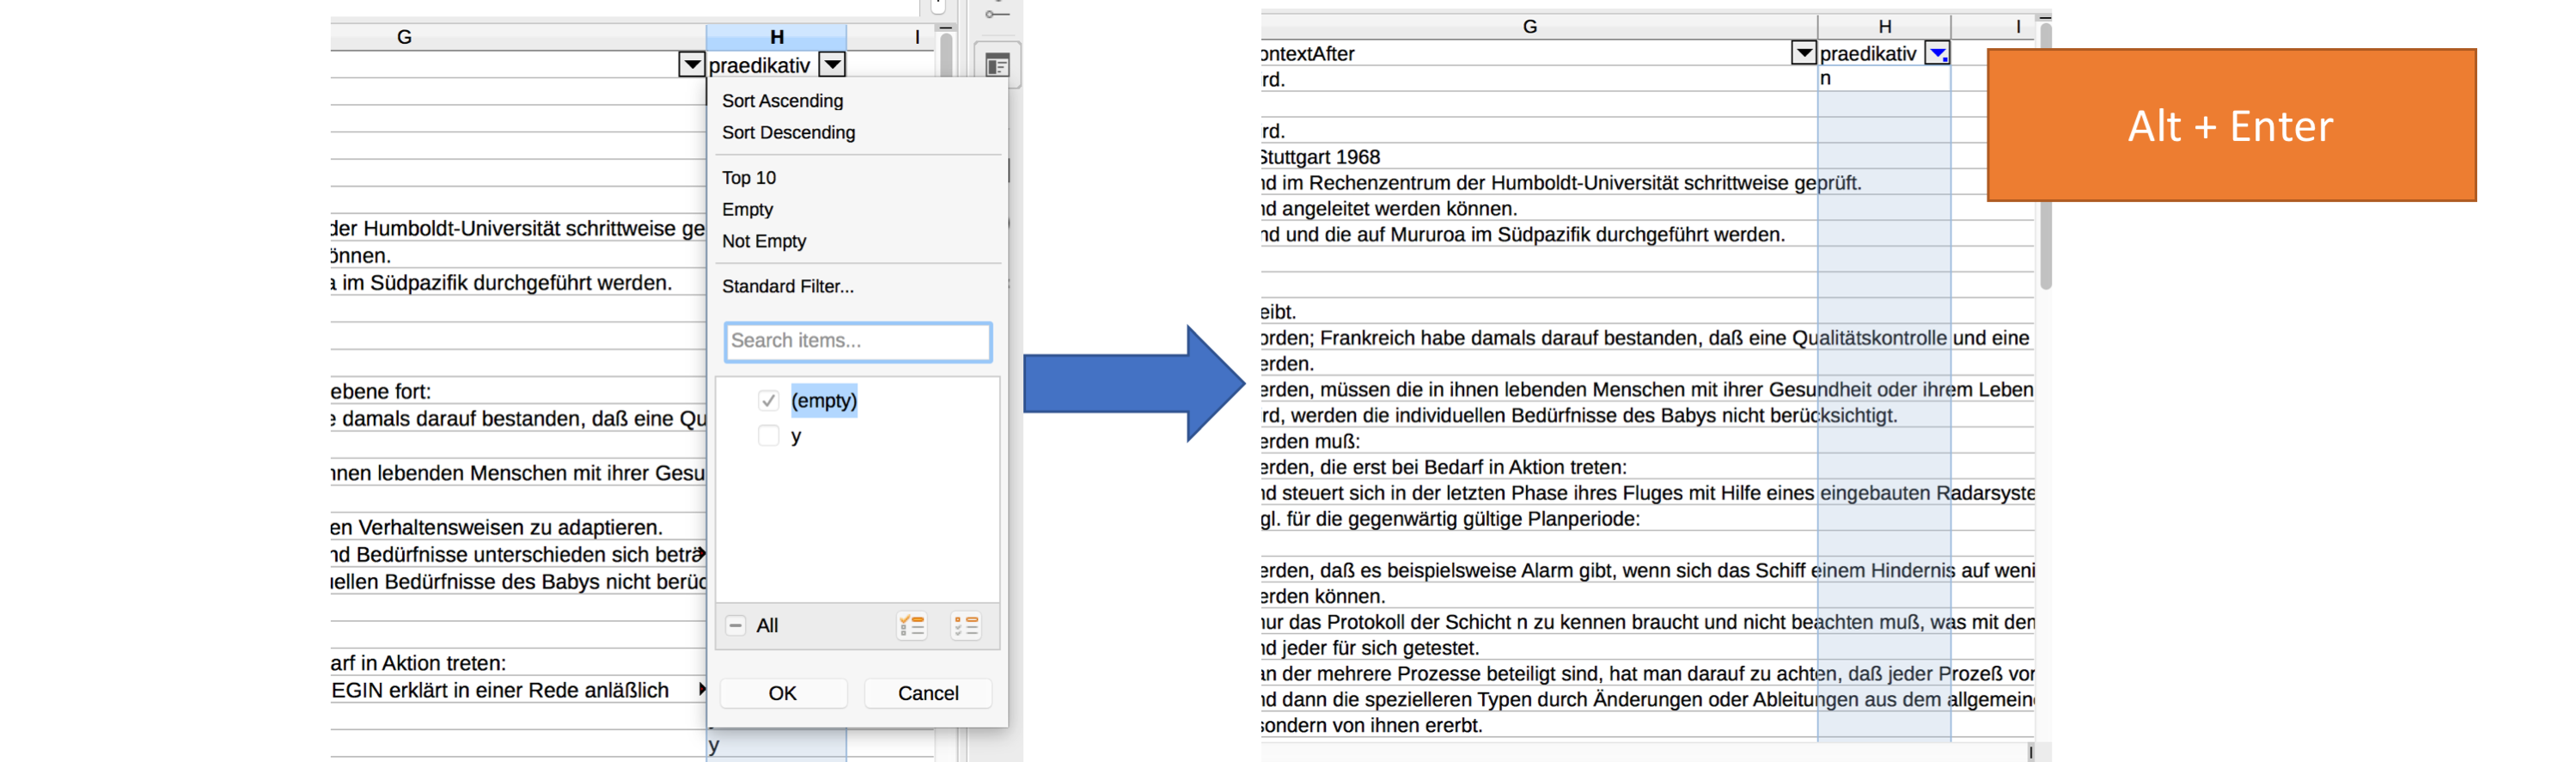
\includegraphics[width=6.66in]{docs/fig/calc_bulkchange} \caption{Eine Tabellenspalte wird so gefiltert, dass nur noch die leeren Zellen zu sehen sind, und allen leeren Zellen wird mit Alt+Enter derselbe Wert zugewiesen.}\label{fig:calcbulkchange}
\end{figure}

Damit ist die Spalte nun vollständig ausgefüllt.

\subsubsection{Annotation metaphorisch
vs.~nicht-metaphorisch}\label{annotation-metaphorisch-vs.nicht-metaphorisch}

Für die weitere Annotation können wir die nicht-prädikativen Fälle außer
Acht lassen. Hier können wir auf die oben erwähnten Filteroptionen
zurückgreifen, um die nicht-prädikativen Fälle herauszufiltern.

Nun gilt es, zu entscheiden, wann \emph{programmiert} und
\emph{vorprogrammiert} metaphorisch verwendet werden und wann nicht.
Auch das ist auf den ersten Blick denkbar einfach: Einen Computer oder
einen Roboter kann man im wörtlichen Sinn programmieren, eine
Katastrophe eher nicht -- allenfalls indirekt, indem man z.B. Maschinen
programmiert, die dann die Weltherrschaft übernehmen, siehe so ziemlich
jede Dystopie von \enquote{Terminator} bis \enquote{Matrix}. Aber genau
dieses indirekte Programmieren bringt uns schon zu möglichen
Zweifelsfällen: Was ist, wenn sich ein Satz wie \emph{Die Konfrontation
ist programmiert} auf einen Roboter bezieht?

Solche Zweifelsfälle ergeben sich gerade bei einer im weitesten Sinne
semantischen Annotation immer. Daher ist es wichtig, klare
\textbf{Annotationsrichtlinien} zu formulieren, in der alle
Annotationsentscheidungen genau dokumentiert sind. Oftmals entwickeln
sich diese Richtlinien im Zuge der Annotation selbst, weil man über
Daten stolpert, die man so zunächst nicht erwartet hätte. (Was übrigens
ein gutes Argument dafür ist, sich bei der Analyse von Sprache nicht
allein auf die eigene Intuition zu verlassen, sondern Korpusdaten zu
Rate zu ziehen!)

Wenn wir nun wörtlichen und metaphorischen Gebrauch annotieren wollen,
könnten unsere Annotationsrichtlinien zunächst ganz einfach so aussehen:

\begin{enumerate}
\def\labelenumi{\arabic{enumi}.}
\item
  Geht aus dem Kontext eindeutig hervor, dass ein Computer bzw. eine
  Maschine programmiert worden ist, liegt wörtlicher Gebrauch vor.
\item
  Geht aus dem Kontext eindeutig hervor, dass sich das Verb auf eine
  andere Entität bezieht, liegt metaphorischer Gebrauch vor.
\item
  Geht aus dem Kontext nicht hervor, worauf genau sich
  \enquote{(vor)programmiert} ist, wird der Beleg als unklar gewertet.
\end{enumerate}

Auf diesen Kriterien aufbauend können wir nun eine neue Spalte in
unserer Tabelle eröffnen, die wir z.B. \enquote{Lesart} nennen können.
Hier vergeben wir die Werte \enquote{lit} (literal/wörtlich),
\enquote{met} (metaphorisch) und \enquote{unklar}. Gerne können Sie es
einmal versuchen und Ihre Ergebnisse dann mit meinen (in den .xlsx- und
.ods-Dateien im \enquote{data}-Ordner) vergleichen.

Der große Vorteil der oben formulierten Annotationskriterien ist, dass
sie sich in den meisten Fällen relativ zweifelsfrei anwenden lassen.
Jedoch zeigt sich beim Durchgehen der konkreten Belege, dass die binäre
Unterscheidung \enquote{wörtlich/metaphorisch} dem Gebrauch von
\emph{(vor)programmiert} möglicherweise nicht ganz gerecht wird. So
fallen die folgenden Beispiele alle in die \enquote{metaphorische}
Kategorie:

\begin{enumerate}
\def\labelenumi{(\arabic{enumi})}
\item
  Der moderne, verbildete Mensch ist nach festen Rhythmen auf das
  eingeschaltete Gerät programmiert und genußbereit.
\item
  Unsere Gene sind auf Lug und Trug programmiert
\item
  da ist Streit mit den Arbeitgebern programmiert.
\end{enumerate}

Die ersten beiden Beispiele bedienen sich der verbreiteten
\enquote{Computermetapher}, konzeptualisieren also den menschlichen
Geist bzw. die menschlichen Gene als \enquote{Computer}. Das ist im
letzten Beispiel nicht der Fall: Hier geht es nicht um das Objekt des
Programmiervorgangs, sondern um das Resultat. Diese Verwendung ist in
gewisser Weise also abstrakter. Das ist allerdings eine Dimension, die
grundsätzlich von der Dimension der wörtlichen vs.~metaphorischen
Verwendung unabhängig ist: Angenommen, ich baue mir, wie es verrückte
Wissenschaftler in Filmen gerne tun, eine Frühstücksmaschine, die so
programmiert ist, dass sie mir morgens um 7 ein Spiegelei brät, und
sage: \enquote{Das Spiegelei ist für 7 programmiert}, dann ist das zwar
eine resultatsbezogene, aber keine metaphorische (sondern eher eine
metonymische) Verwendung.

Es wäre daher sinnvoll, auch diese Dimension noch zu kodieren.\footnote{Der
  Vollständigkeit halber sei darauf hingewiesen, dass es sich dabei um
  eine Post-hoc-Analyse handelt. Wenn Sie sich ein wenig in die
  Wissenschaftsphilosophie einlesen, werden Sie merken, dass so etwas
  nicht unumstritten ist: Oft gilt es als Ideal, sämtliche Hypothesen
  und Analysemethoden im Voraus festzulegen, bevor man sich den Daten
  selbst zuwendet. \emph{Post hoc} aufgestellte Hypothesen müsste man
  dann eigentlich anhand von neuen Daten überprüfen. De facto ist es
  freilich oft so, dass für so ein rigides Vorgehen Zeit und Ressourcen
  fehlen. Gerade bei einer Seminararbeit können Sie diesen Punkt
  natürlich in aller Regel getrost ignorieren.} Deshalb fügen wir noch
eine weitere Annotationsspalte hinzu, die wir \enquote{Referenz} nennen:
Referiert der fragliche Satz auf das, was programmiert wird, oder auf
das Resultat der Programmierung?

Auch hierfür formulieren wir wieder Annotationskriterien:

\begin{enumerate}
\def\labelenumi{\arabic{enumi}.}
\item
  Wenn aus dem Kontext eindeutig hervorgeht, dass sich der Satz auf das
  Objekt des Programmiervorgangs bezieht (\emph{der Computer ist
  programmiert} \enquote{jemand (Subj.) hat den Computer (Obj.)
  programmiert}), wird der Beleg mit \enquote{obj} annotiert.
\item
  Wenn aus dem Kontext eindeutig hervorgeht, dass sich der Satz auf das
  Resultat des (ggf. stark metaphorischen) Programmiervorgangs bezieht
  (\emph{das Spiegelei ist programmiert} \enquote{jemand hat die
  Frühstücksmaschine so programmiert, dass sie ein Spiegelei (Resultat)
  macht} oder \emph{die Katastrophe ist programmiert} \enquote{es wurden
  Entscheidungen getroffen, die zwangsläufig in eine Katastrophe
  (Resultat) führen}), so wird der Beleg mit \enquote{res} annotiert.
\item
  Lässt sich keine eindeutige Entscheidung treffen, bekommt der Beleg
  den Wert \enquote{unklar}.
\end{enumerate}

In den .xlsx- und .odt-Dateien im \enquote{data}-Ordner habe ich das in
der Spalte \enquote{Referenz} umgesetzt. Auch hier können Sie gern die
Probe aufs Exempel machen und überprüfen, ob Ihre Annotationen mit
meinen übereinstimmen. Wahrscheinlich werden Sie im einen oder anderen
Fall andere Entscheidungen treffen als ich -- das ist ganz normal und
auch der Grund dafür, warum man idealerweise mindestens zwei Personen
unabhängig voneinander annotieren lassen und dann die Annotationen
vergleichen sollte. (De facto ist das natürlich gerade bei einer
Seminararbeit häufig nicht möglich).

\subsection{Auswertung und
Visualisierung}\label{auswertung-und-visualisierung}

Nachdem wir nun die Daten annotiert haben, können wir unsere
Annotationen quantitativ auswerten. Auch hier zeige ich wieder die
einzelnen Wege für Excel und Calc auf.

\subsubsection{Auswertung und Visualisierung in
Excel}\label{auswertung-und-visualisierung-in-excel}

Ideal für die Auswertung und Visualisierung in Excel ist die
PivotTable-Funktion. Manches an dieser Funktion ist zunächst ein wenig
gewöhnungsbedürftig, aber nach kurzer Eingewöhnungszeit ist sie doch
halbwegs logisch und intuitiv.

Stellen Sie zunächst sicher, dass eine Zelle innerhalb der Tabelle
angewählt ist (z.B. die Zelle ganz oben links). Jetzt klicken wir im
Reiter \enquote{Einfügen} auf \enquote{PivotTable}. Nun öffnet sich ein
Fenster, in dem wir gefragt werden, welche Zellen Teil der PivotTable
werden sollen (hier sollte Excel bereits automatisch erkannt haben, dass
wir die ganze Tabelle einbeziehen wollen, sodass wir nichts mehr ändern
müssen) und ob die Tabelle auf dem aktuellen oder einem neuen
Arbeitsblatt erstellt werden soll -- es empfiehlt sich, sie auf einem
neuen Arbeitsblatt zu erstellen, was auch die Default-Option ist. Also
können wir einfach OK klicken. In der HTML-Version dieses Tutorials
können Sie die einzelnen Schritte in Screencast \ref{fig:excelpivot}
nachverfolgen.

\begin{figure}
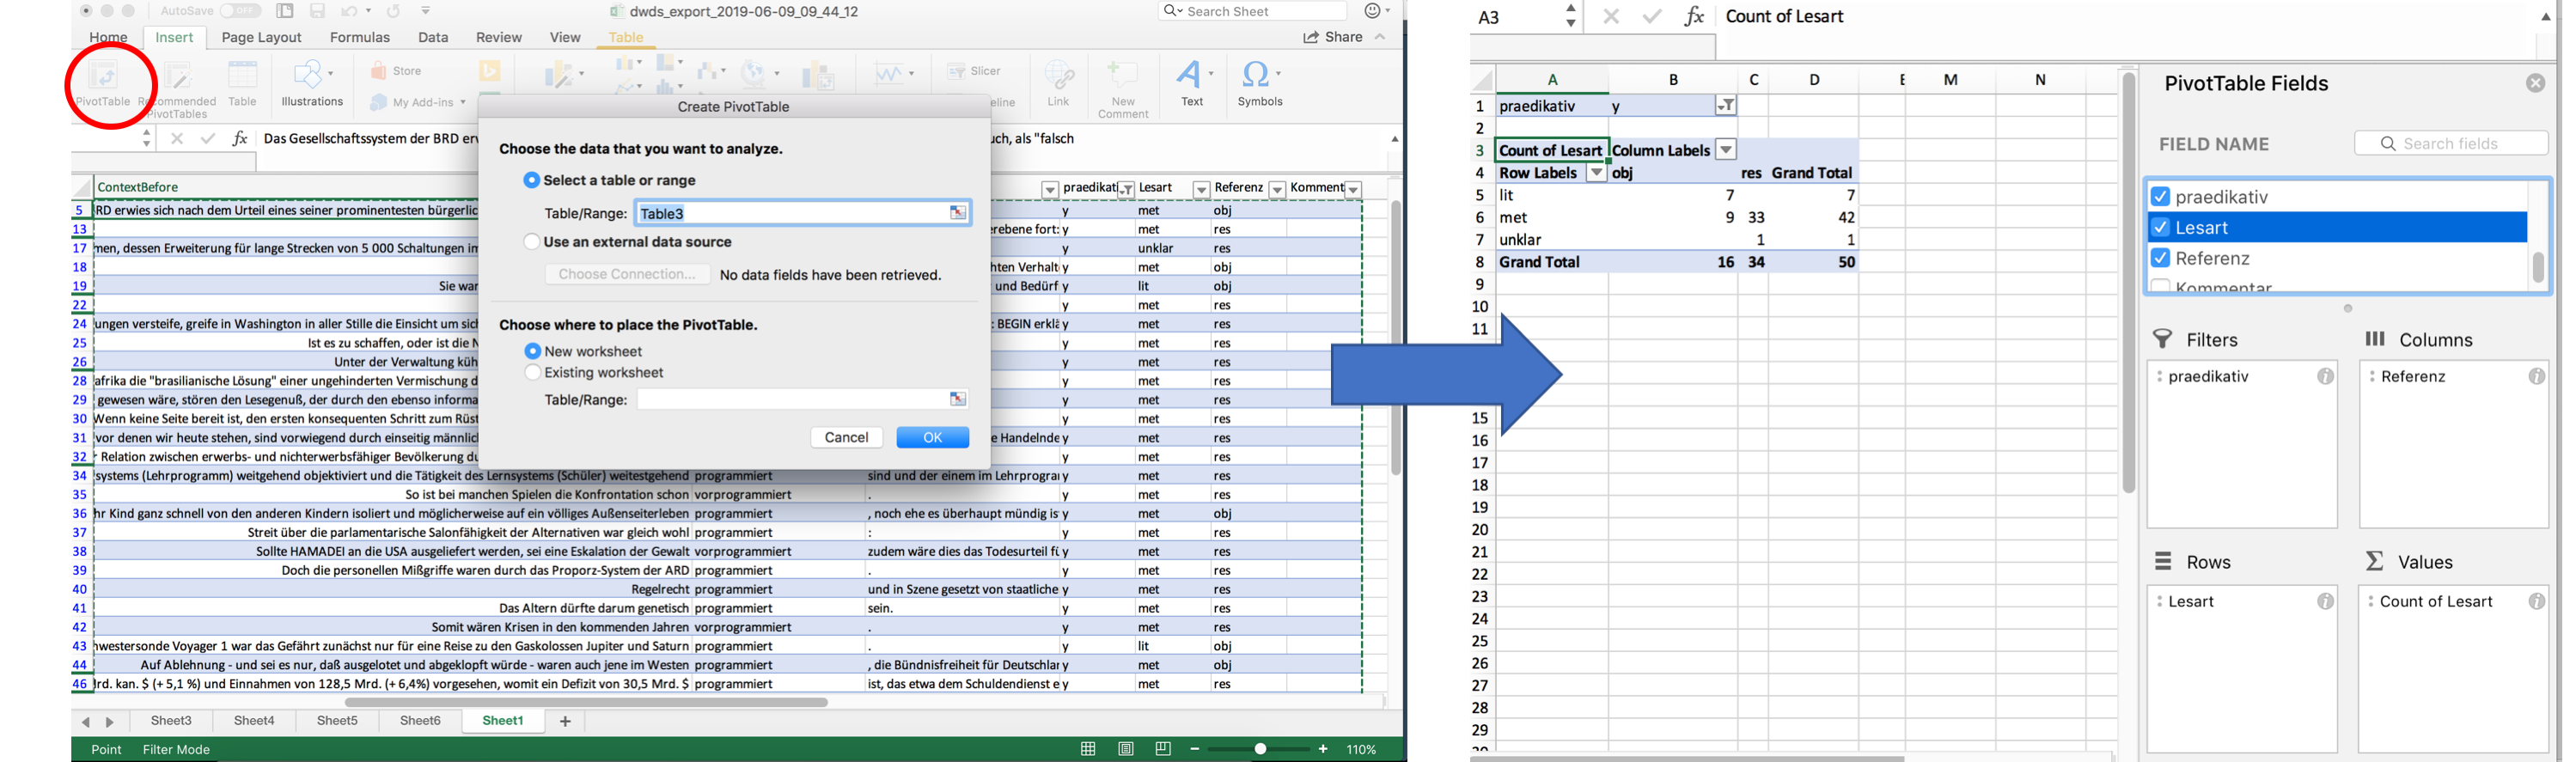
\includegraphics[width=6.66in]{docs/fig/excelpivot} \caption{Erstellen einer Pivot-Tabelle in Excel.}\label{fig:excelpivot}
\end{figure}

Nun öffnet sich ein neues Arbeitsblatt (mit den Reitern unten können Sie
zwischen den Arbeitsblättern navigieren und ihnen ggf. auch
aussagekräftigere Namen geben). Wir sehen ein dreigeteiltes Fenster. Im
Arbeitsblatt selbst finden wir ein etwas kryptisch aussehendes, noch
weitgehend leeres Feld mit einer Beschriftung wie \enquote{PivotTable1}
o.ä. Das ist quasi der Platzhalter für die noch zu erstellende Tabelle.
Rechts sehen wir oben eine Aufstellung der Namen der Tabellenspalten,
unten sehen wir ein wiederum viergeteiltes Fenster. In die vier Felder
in diesem Fenster können wir nun ausgewählte Spaltennamen aus dem
Fenster oben rechts ziehen. Probieren Sie doch einmal, die Spalte
\enquote{Hit} in das Feld \enquote{Zeilen} zu ziehen. Jetzt sehen Sie in
der Pivot-Tabelle die beiden Zeilen \enquote{programmiert} und
\enquote{vorprogrammiert}. Höchstwahrscheinlich ist \enquote{Hit} auch
automatisch im Fenster \enquote{Werte} unten rechts aufgetaucht. Deshalb
wird Ihnen in der Pivot-Tabelle auch die Häufigkeit der beiden Varianten
angezeigt, wie in \ref{fig:excelpivotsimple}.

\begin{figure}
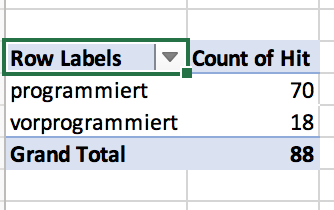
\includegraphics[width=1.11in]{docs/fig/excel_simplepivot} \caption{Eine Pivot-Tabelle in Excel.}\label{fig:excelpivotsimple}
\end{figure}

Die Logik ist also ganz einfach: Was im Feld \enquote{Spalten} steht,
taucht in den Spalten der Tabelle auf, was im Feld \enquote{Zeilen}
steht, taucht in den Zeilen auf, und was im Feld \enquote{Werte} steht,
das wird ausgezählt\footnote{bzw. bei numerischen Werten aufsummiert;
  hier muss man ggf. aufpassen, dass die richtige Operation gewählt ist.
  Durch Klick auf das kleine Info-Symbol in den Feldern kann man das bei
  Bedarf anpassen}. Mit Hilfe des Felds \enquote{Filter} kann man die
Daten bei Bedarf filtern.

In unserem Beispiel wollen wir genau das tun: Wir wollen ja nur die
prädikativ gebrauchten Instanzen von \emph{(vor)programmiert}
berücksichtigen. Leeren wir die beiden Felder zunächst wieder, indem wir
\enquote{Hit} aus dem jeweiligen Feld in das Fenster rechts oben ziehen
(Fig. \ref{fig:countofhit}).

\begin{figure}
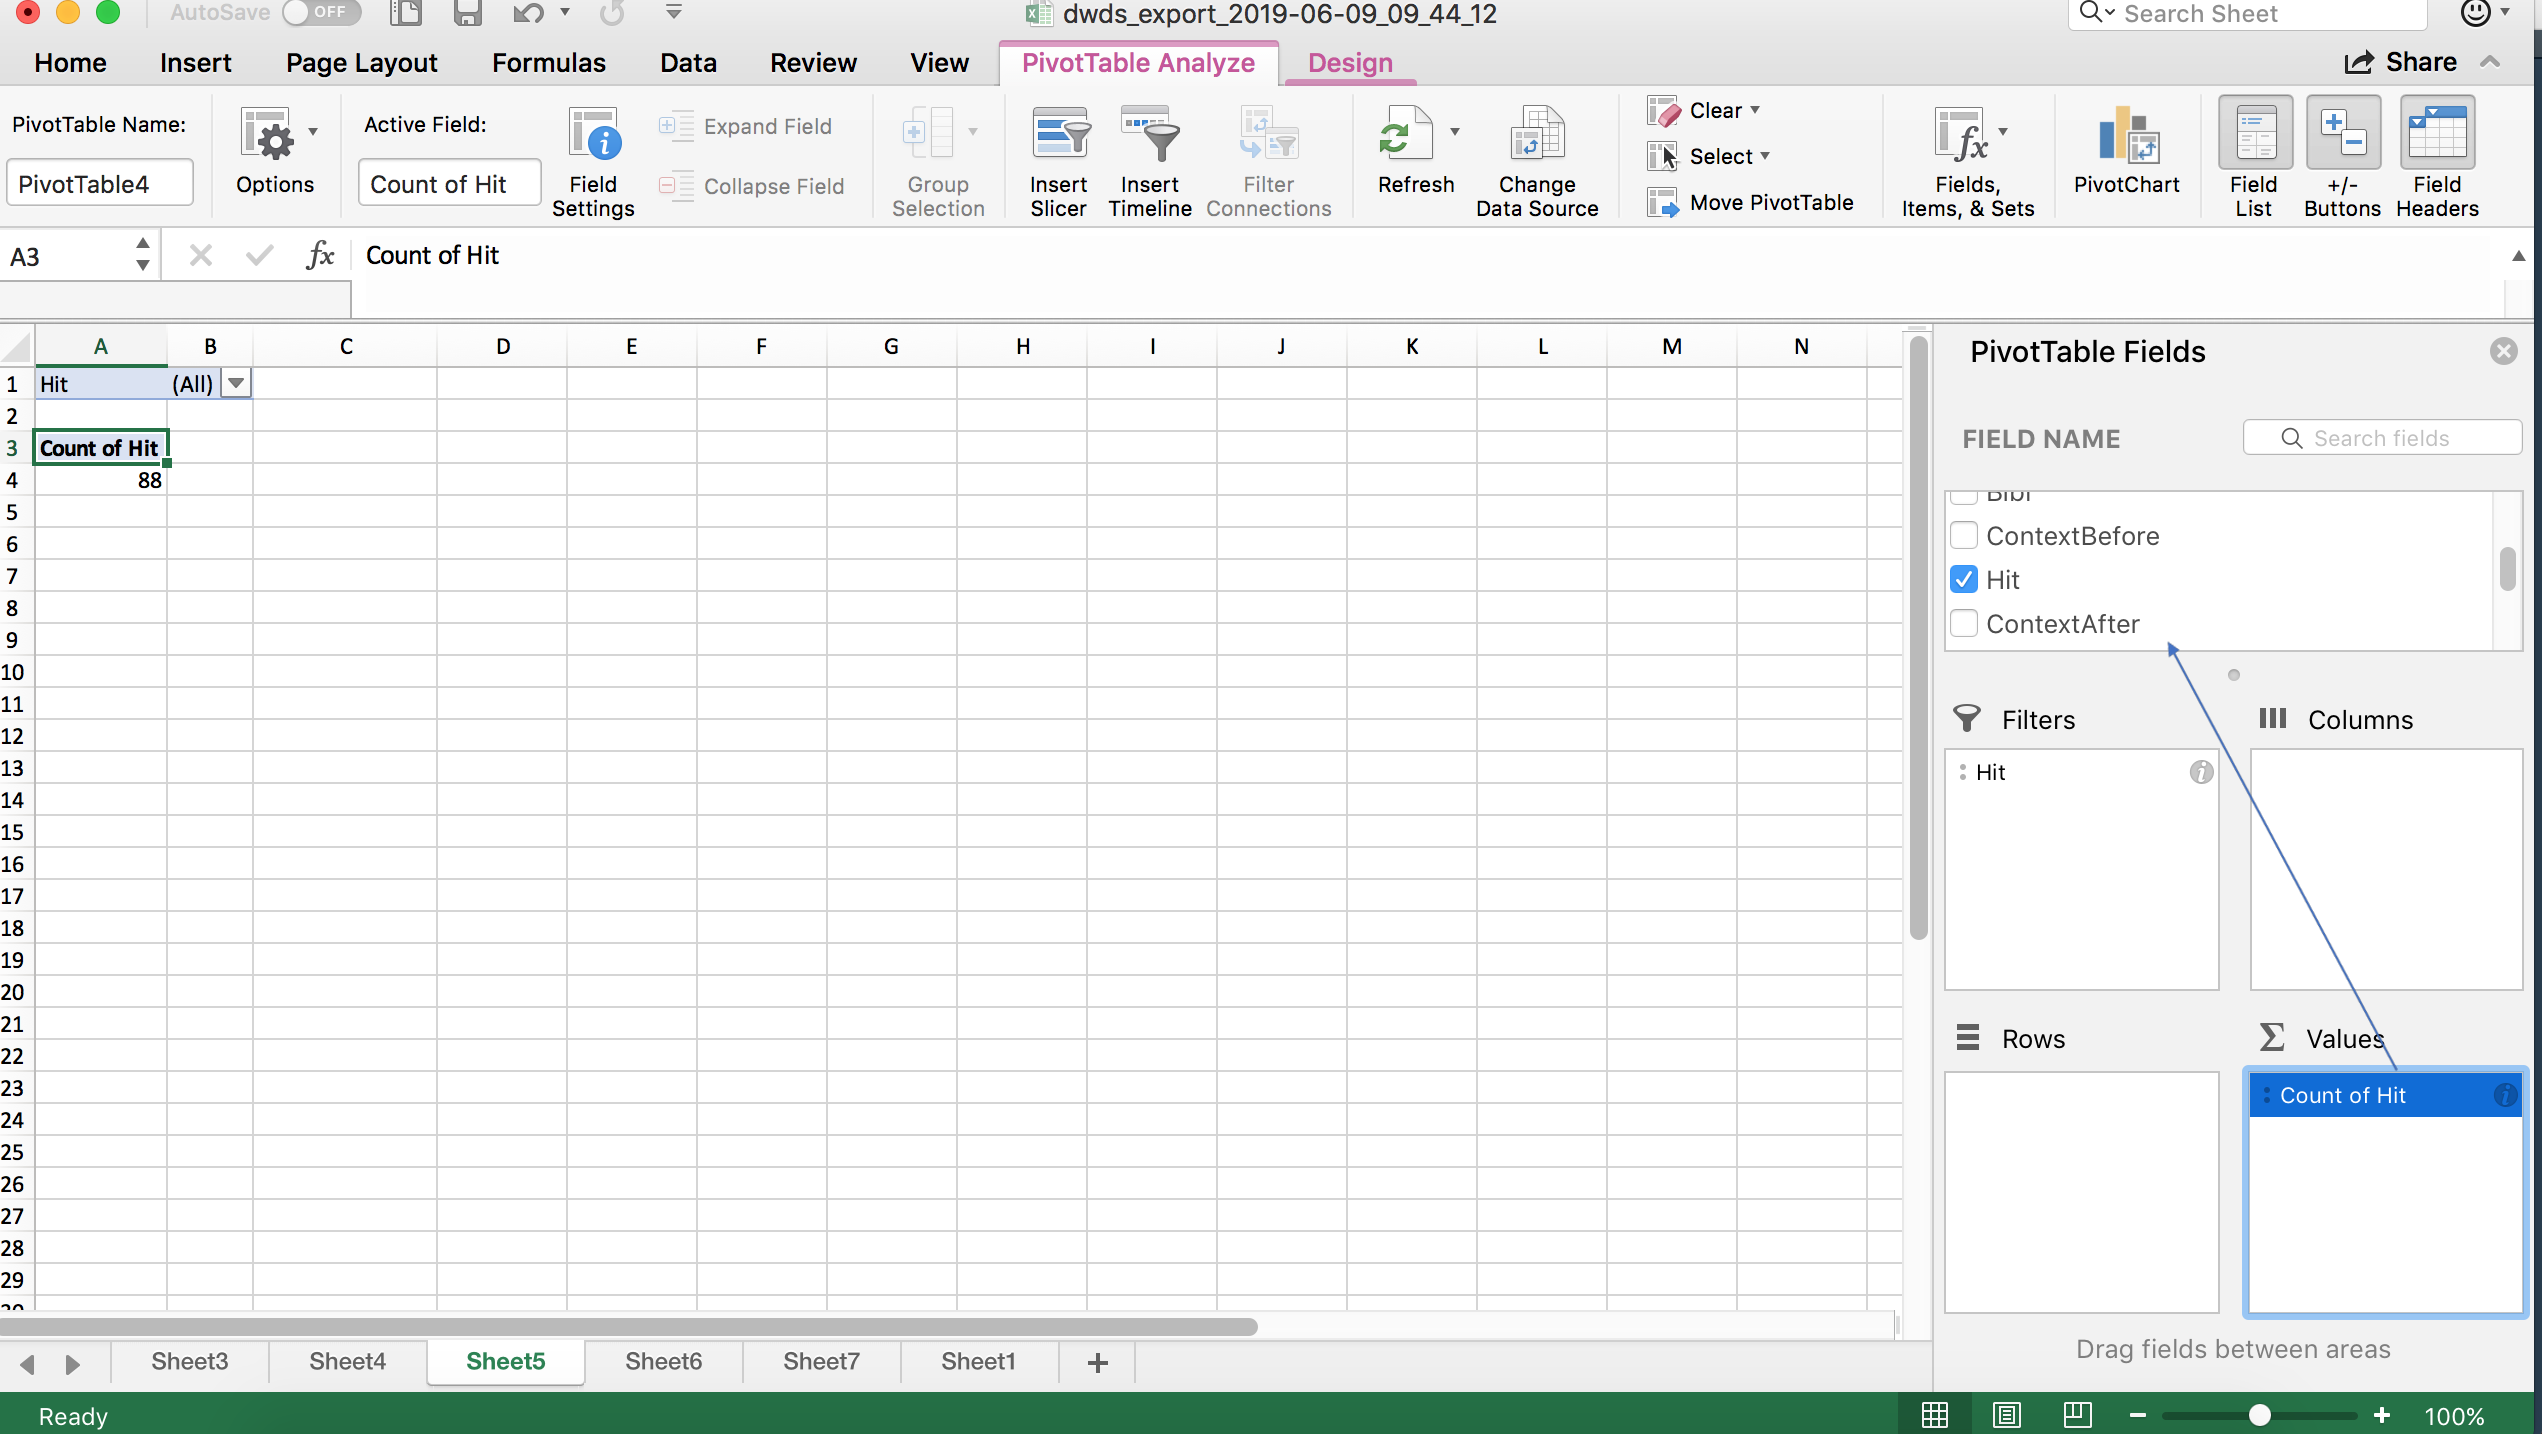
\includegraphics[width=6.36in]{docs/fig/countofhit} \caption{Entfernen einer Spalte aus dem "Werte"-Feld.}\label{fig:countofhit}
\end{figure}

Dann ziehen wir die Spalte \enquote{prädikativ} in das Feld
\enquote{Filter}. Jetzt können wir im Fenster links die
nicht-prädikativen Daten herausfiltern (s. Fig.
\ref{fig:praedikativfilter}).

\begin{figure}
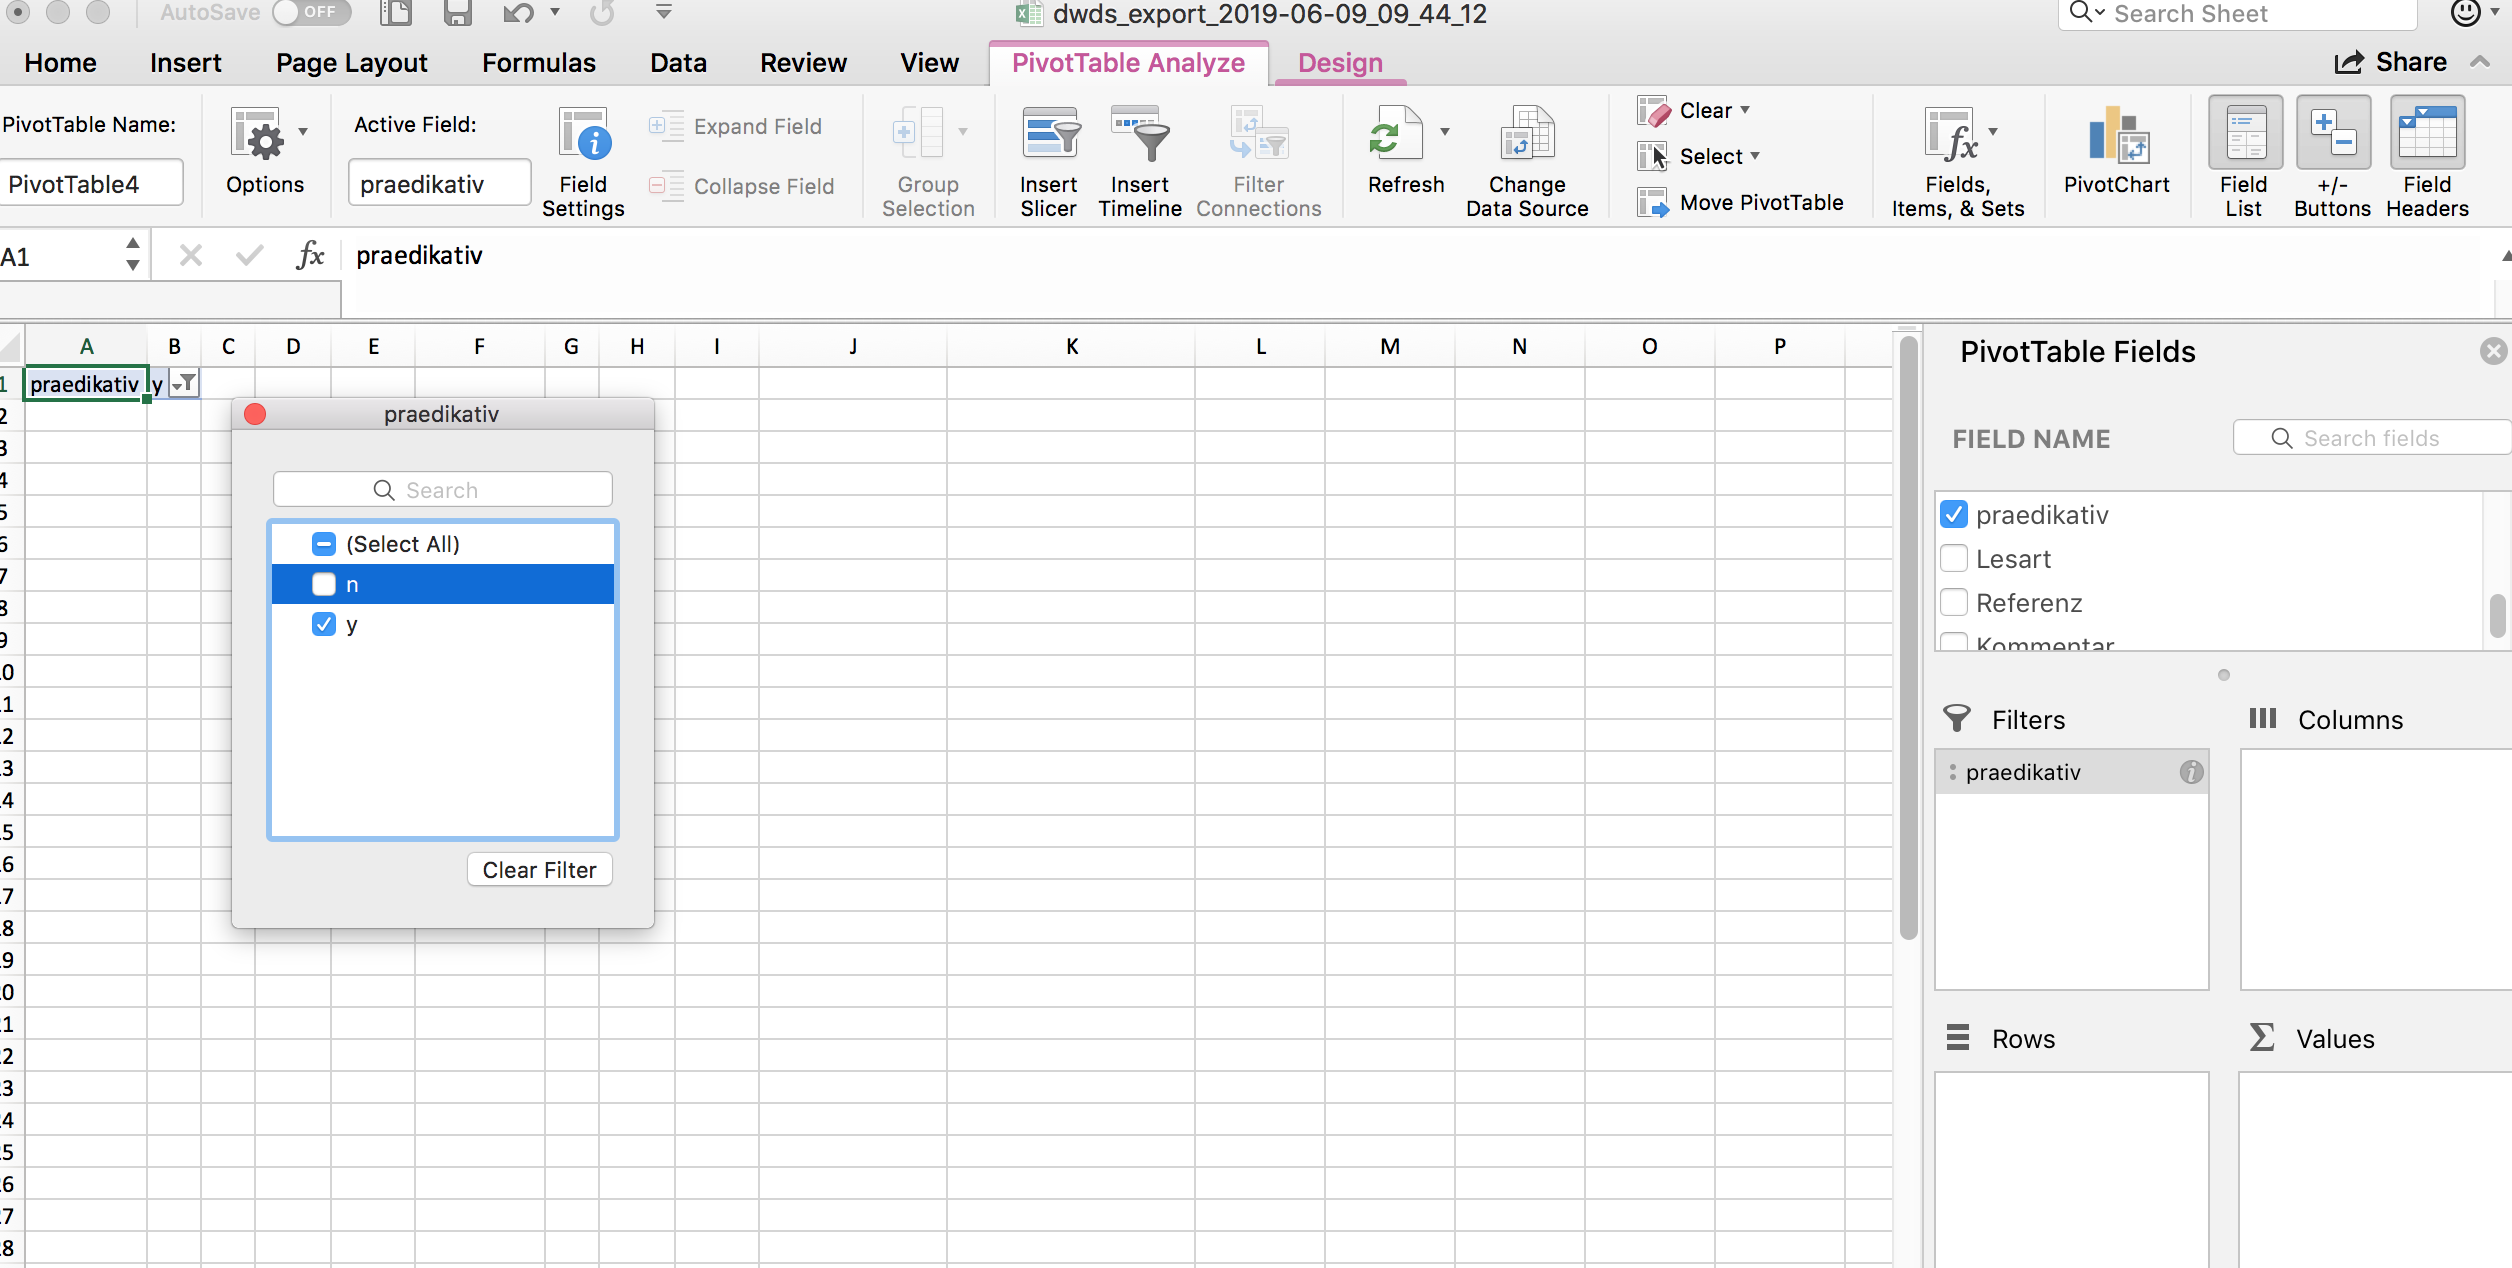
\includegraphics[width=6.28in]{docs/fig/praedikativ_filter} \caption{Herausfiltern der Daten mit "praedikativ=n".}\label{fig:praedikativfilter}
\end{figure}

Nun wollen wir eine tabellarische Übersicht über die Lesarten und die
Referenz (Objekt vs.~Resultat) getrennt nach den beiden Varianten
\enquote{programmiert} und \enquote{vorprogrammiert} bekommen. Führen
wir uns noch einmal vor Augen, was die dafür relevanten Tabellenspalten
sind:

\begin{itemize}
\tightlist
\item
  Die Spalte \enquote{Lesart} enthält die Lesarten.
\item
  Die Spalte \enquote{Referenz} enthält die Information darüber, ob der
  jeweilige Beleg auf das Objekt des Programmiervorgangs oder dessen
  Resultat referiert.
\item
  Die Spalte \enquote{Hit} enthält die Variante des Treffers.
\end{itemize}

Zur Auswertung müssen wir die drei Spalten nun sinnvoll auf die
\enquote{Zeilen}- und \enquote{Spalten}-Felder verteilen und zudem
angeben, was ausgezählt werden soll. Hier gibt es mehrere Möglichkeiten;
eine davon ist in \ref{fig:excelfilter} dargestellt: In den Spalten
werden die Daten nach Variante (\enquote{Hit}) ausgewertet, in den
Zeilen zum einen nach Lesart, zum anderen nach Referenz. Ausgezählt wird
die Spalte \enquote{Lesart} -- genauso gut könnten wir aber auch die
Spalte \enquote{Referenz} auszählen, die Ergebnisse wären die gleichen,
da ja beide Variablen in der Tabelle berücksichtigt sind.

\begin{figure}
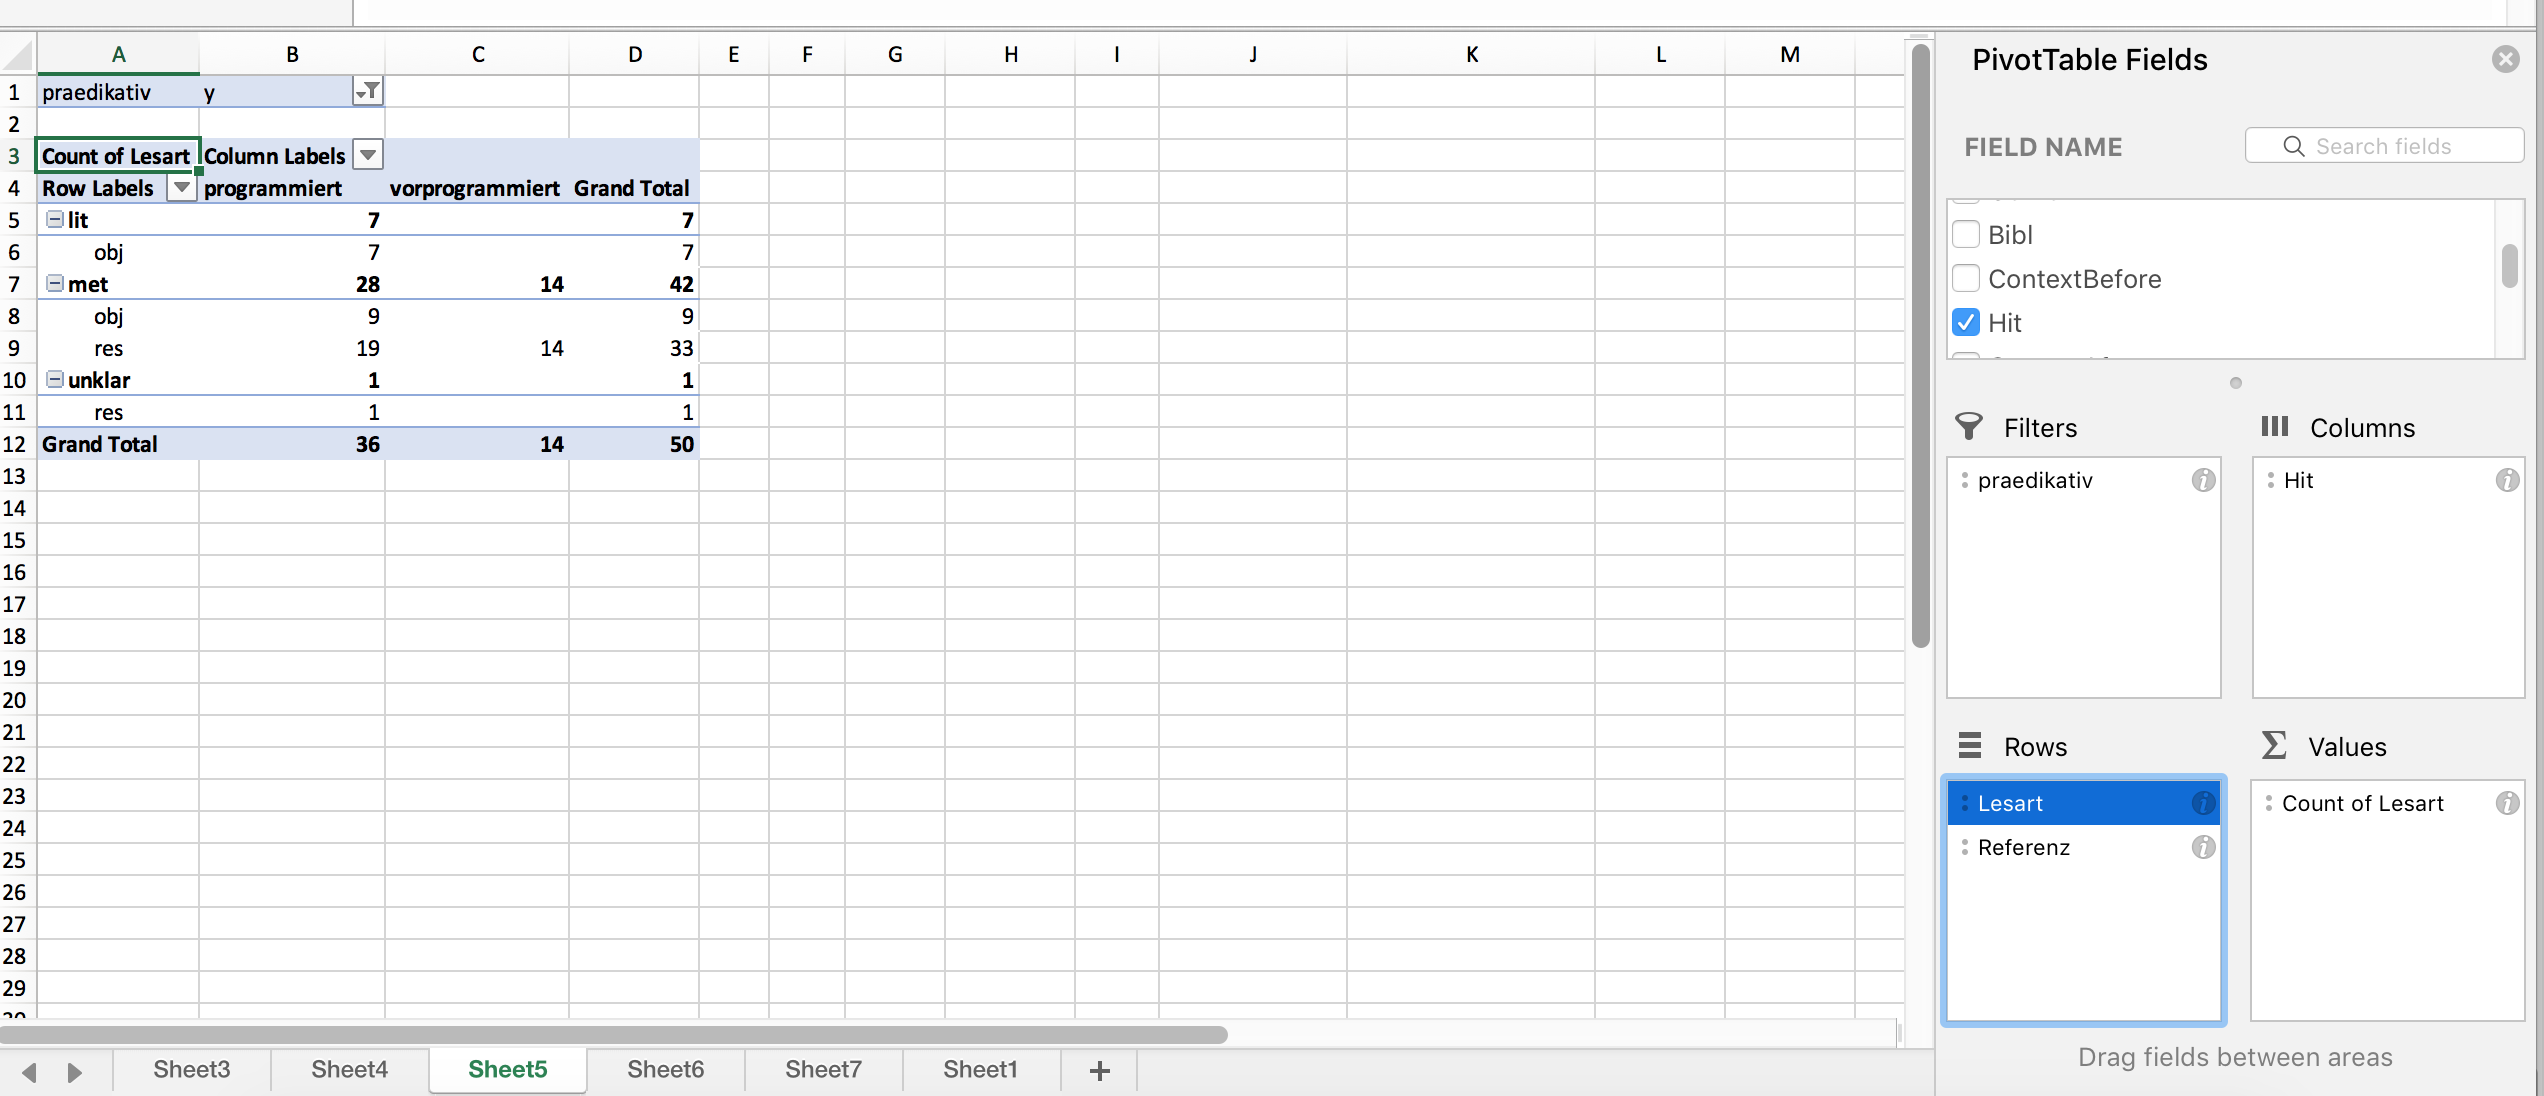
\includegraphics[width=6.36in]{docs/fig/excel_allfilters} \caption{Tabellarische Auswertung der Korpusdaten mit Hilfe der PivotTable-Funktion.}\label{fig:excelfilter}
\end{figure}

Schon auf den ersten Blick sehen wir eine ungleiche Verteilung der Daten
auf die beiden Varianten: \emph{vorprogrammiert} wird in unseren Daten
ausschließlich in metaphorischen Kontexten und ausschließlich für
Resultate gebraucht. Bei \emph{programmiert} ist der Gebrauch
vielfältiger, wenngleich auch hier eine Präferenz für eben diese
Merkmalskombination (metaphorischer Kontext/Resultat) deutlich wird.

Quasi als Sahnehäubchen können wir diese Verteilung auch visualisieren,
beispielsweise mit einem Balkendiagramm.\footnote{Vgl. jedoch z.B. diese
  Seite zu Problemen, die Balkendiagramme u.U. mit sich bringen.} Das
geht, indem wir die relevanten Zellen in der PivotTable markieren (also
alles, was nicht die Gesamtsumme anzeigt) und dann in \enquote{Einfügen}
eine passende Visualisierungsoption auswählen. \ref{fig:excelvisualize}
zeigt eine Möglichkeit, das umzusetzen:

\begin{figure}
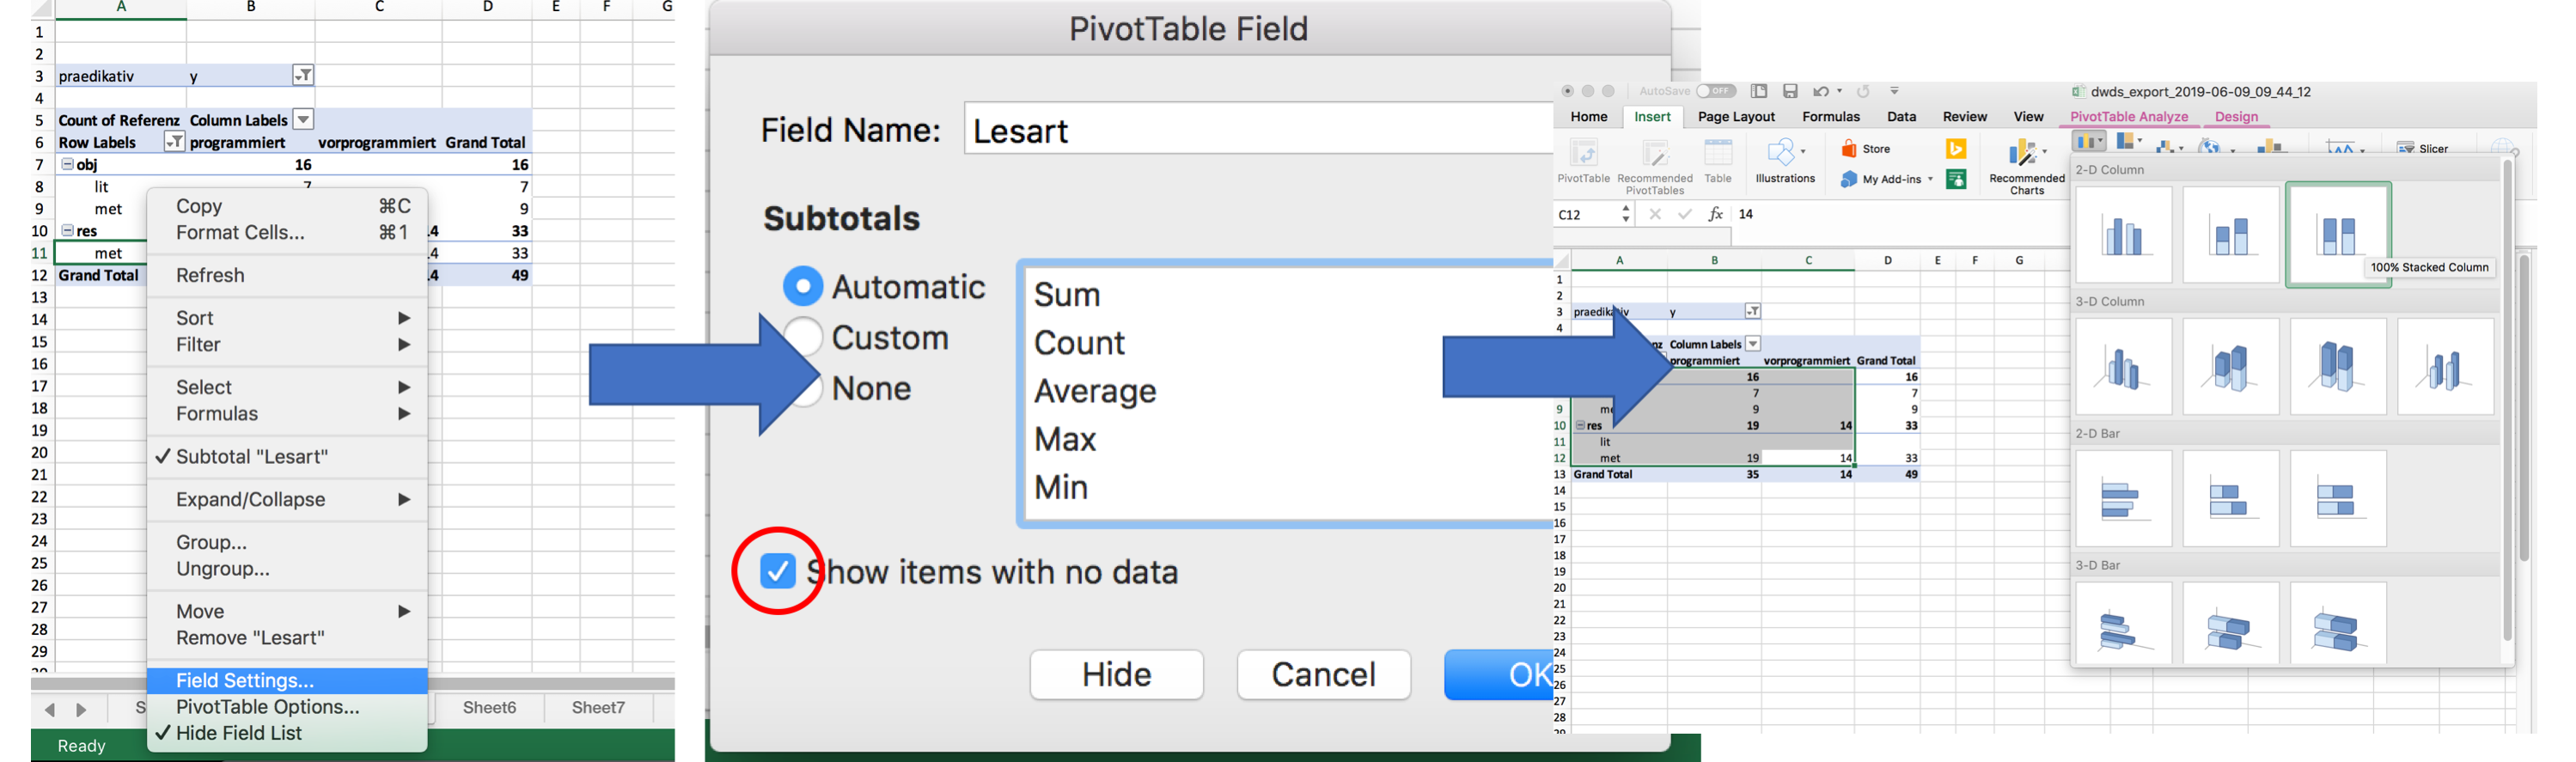
\includegraphics[width=6.66in]{docs/fig/excel_visualize} \caption{Erstellen eines Balkendiagramms aus einer Pivot-Tabelle in Excel.}\label{fig:excelvisualize}
\end{figure}

Welche Daten auf der x- und auf der y-Achse dargestellt und welche
innerhalb der Balken farblich kodiert werden, hängt davon ab, welche
Daten in der Pivot-Tabelle in den Zeilen und in den Spalten stehen.
Gegebenenfalls kann man hier noch ein paar Änderungen vornehmen, um die
Darstellung sinnvoller zu gestalten. So entsteht in Fig.
\ref{fig:excelvisualize} ein Diagramm, bei dem die Variante
(\emph{programmiert} vs. \emph{vorprogrammiert}) farblich kodiert wird.
Das ist nicht unbedingt sinnvoll, weil wir ja wissen wollen, wie sich
die Verteilung der unterschiedlichen Lesarten zwischen den beiden
Varianten unterscheidet. Man kann die visuelle Darstellung auch in dem
\enquote{Pivot Chart Fields}-Feld ändern, das sich bei der Erstellung
des Balkendiagramms geöffnet haben dürfte (\ref{fig:pivotchartfields}).

\begin{figure}
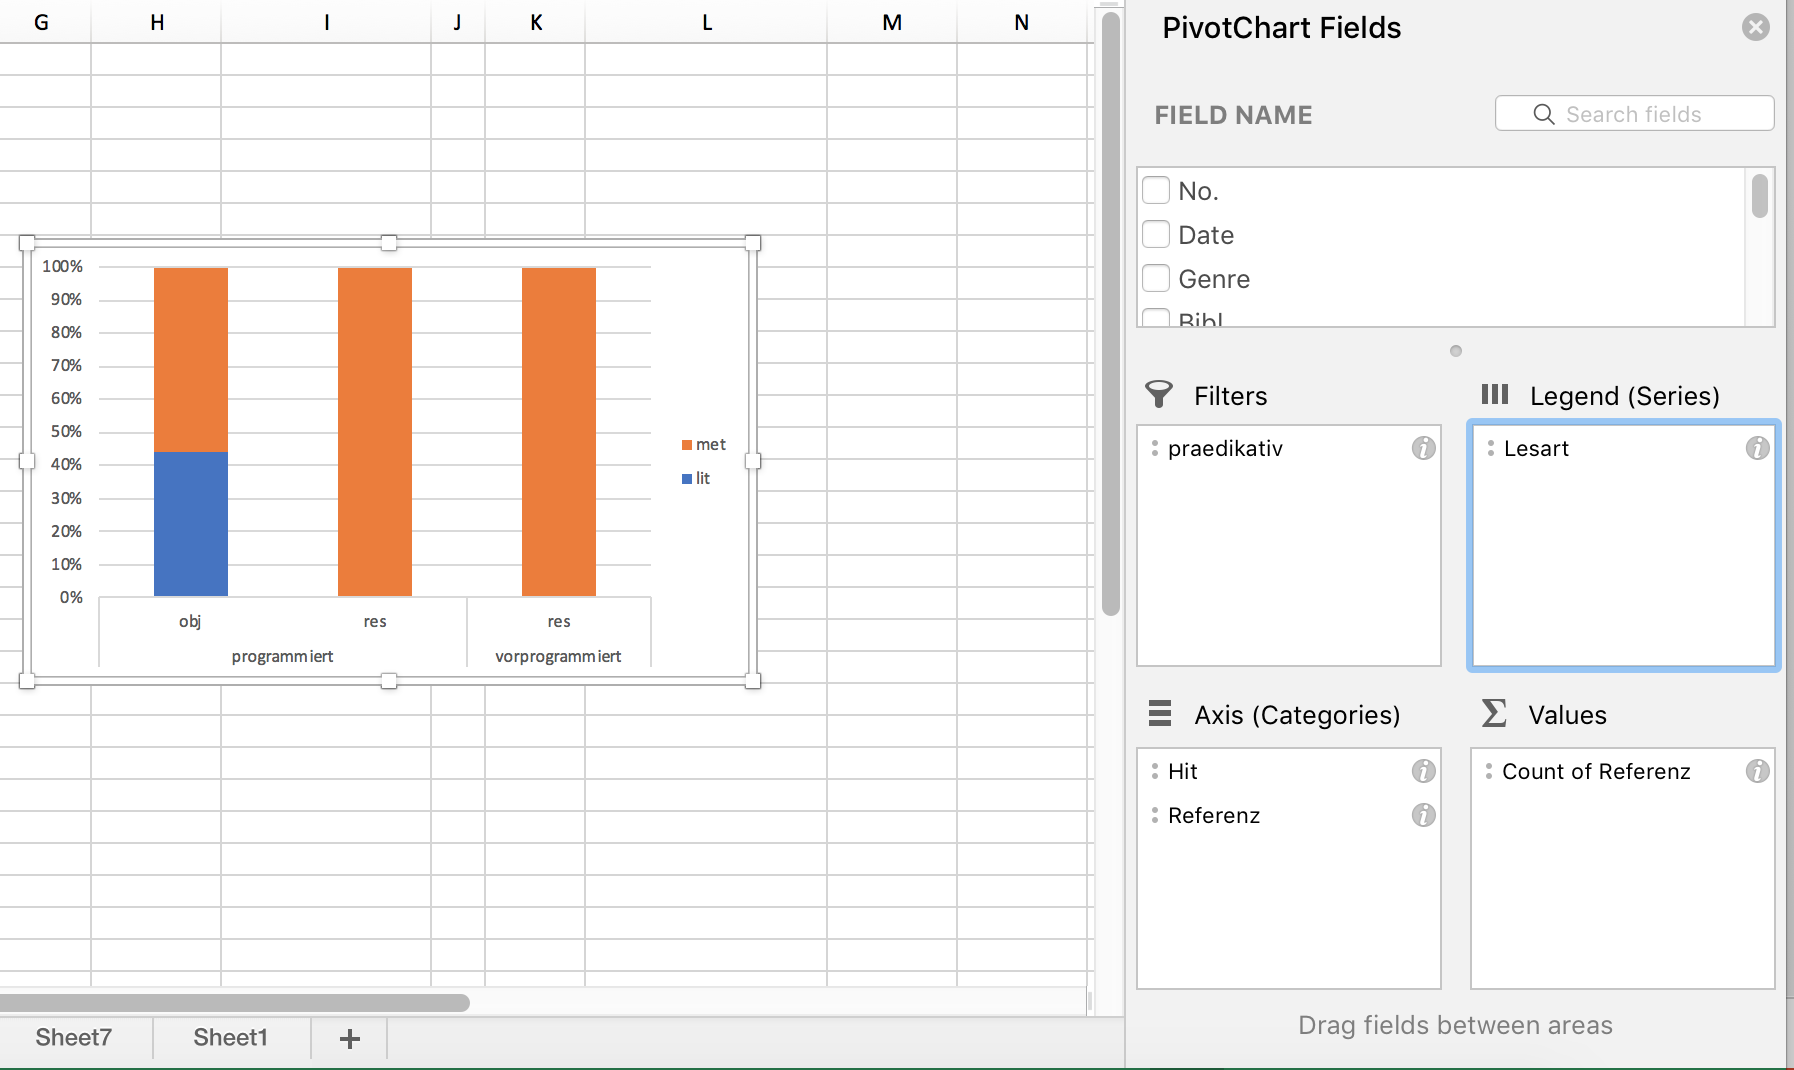
\includegraphics[width=4.49in]{docs/fig/excel_pivotchartfields} \caption{Der Dialog "Pivot Chart Fields" (rechts) erlaubt es, anzupassen, was wo in der Grafik dargestellt wird.}\label{fig:pivotchartfields}
\end{figure}

Und noch etwas Feinjustierung: Damit die Grafik nicht so asymmetrisch
aussieht wie Fig. \ref{fig:asymmetric}, werden (im ersten Schritt in
\ref{fig:excelvisualize}) zunächst die Feldeinstellungen so verändert,
dass auch Felder mit Null-Werten angezeigt werden. Anschließend wird ein
Balkendiagramm ausgewählt, das den prozentualen Anteil der jeweiligen
Variante darstellt. Durch Rechtsklick auf die Balken kann man außerdem
noch \enquote{Data Labels} hinzufügen, d.h. die absoluten Werte in den
Balken darstellen lassen. Das ist empfehlenswert, weil so die Leserin
oder der Leser schnell einen Eindruck gewinnen kann, wie groß die
Datenbasis ist, auf der die Darstellung basiert -- denn es macht ja
schon einen gewichtigen Unterschied, ob eine Verteilung wie, sagen wir
10\% : 90\% auf zehn, auf hundert oder auf tausend Datenpunkten basiert!
Die \enquote{Data Labels} kann man hinzufügen durch Rechtsklick auf die
Balken und Klick auf den Punkt \enquote{Show data labels}.

\begin{figure}
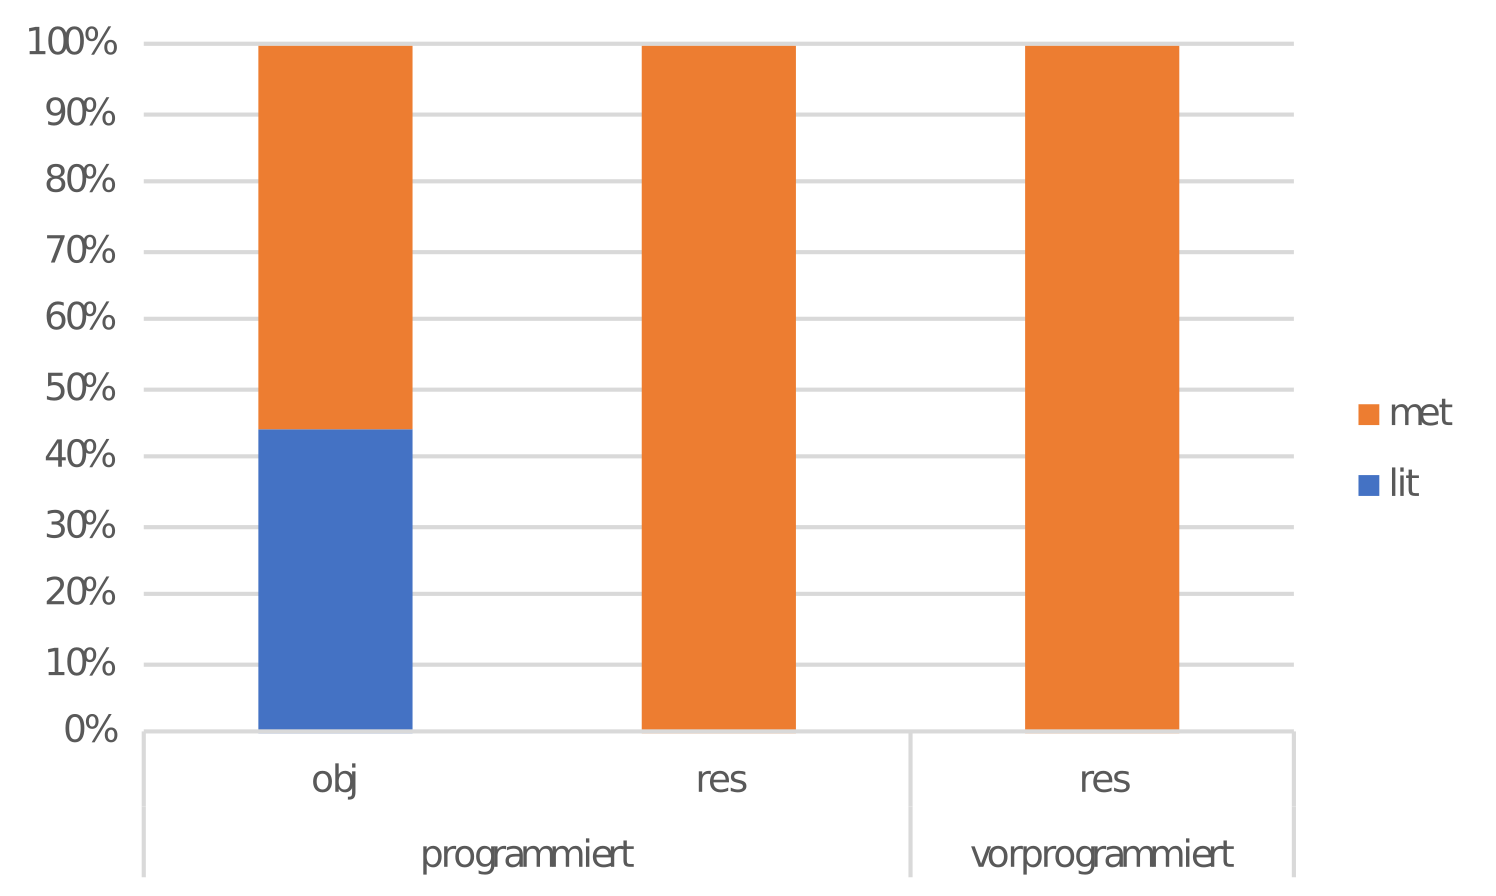
\includegraphics[width=3.32in]{docs/fig/excel_asymmetric} \caption{Balkendiagramm, in dem nicht belegte Variablenausprägungen ausgelassen werden.}\label{fig:asymmetric}
\end{figure}

\subsubsection{Auswertung und Visualisierung in
Calc}\label{auswertung-und-visualisierung-in-calc}

Auch in Calc gibt es eine PivotTable-Funktion, die sich im Dropdown-Menü
\enquote{Data} findet. Mit Hilfe von PivotTable \textgreater{} Erstellen
gelangt man in ein Auswahlmenü, in dem rechts die einzelnen Spaltennamen
als \enquote{available fields} zu sehen sind. Links sehen wir drei
rechteckige Felder: eins für Zeilen, eins für Spalten und eins für Werte
(das Letztere trägt die nicht ganz so aussagekräftige Überschrift
\enquote{Data fields}). Aus der Auflistung rechts können wir nun die
Variablen, die wir in den Spalten sehen wollen, ins
\enquote{Spalten}-Feld ziehen, diejenigen, die wir in den Zeilen sehen
wollen, ins \enquote{Zeilen}-Feld und schließlich diejenigen, die Calc
für uns auszählen soll, ins \enquote{Data fields}-Feld.

\begin{figure}
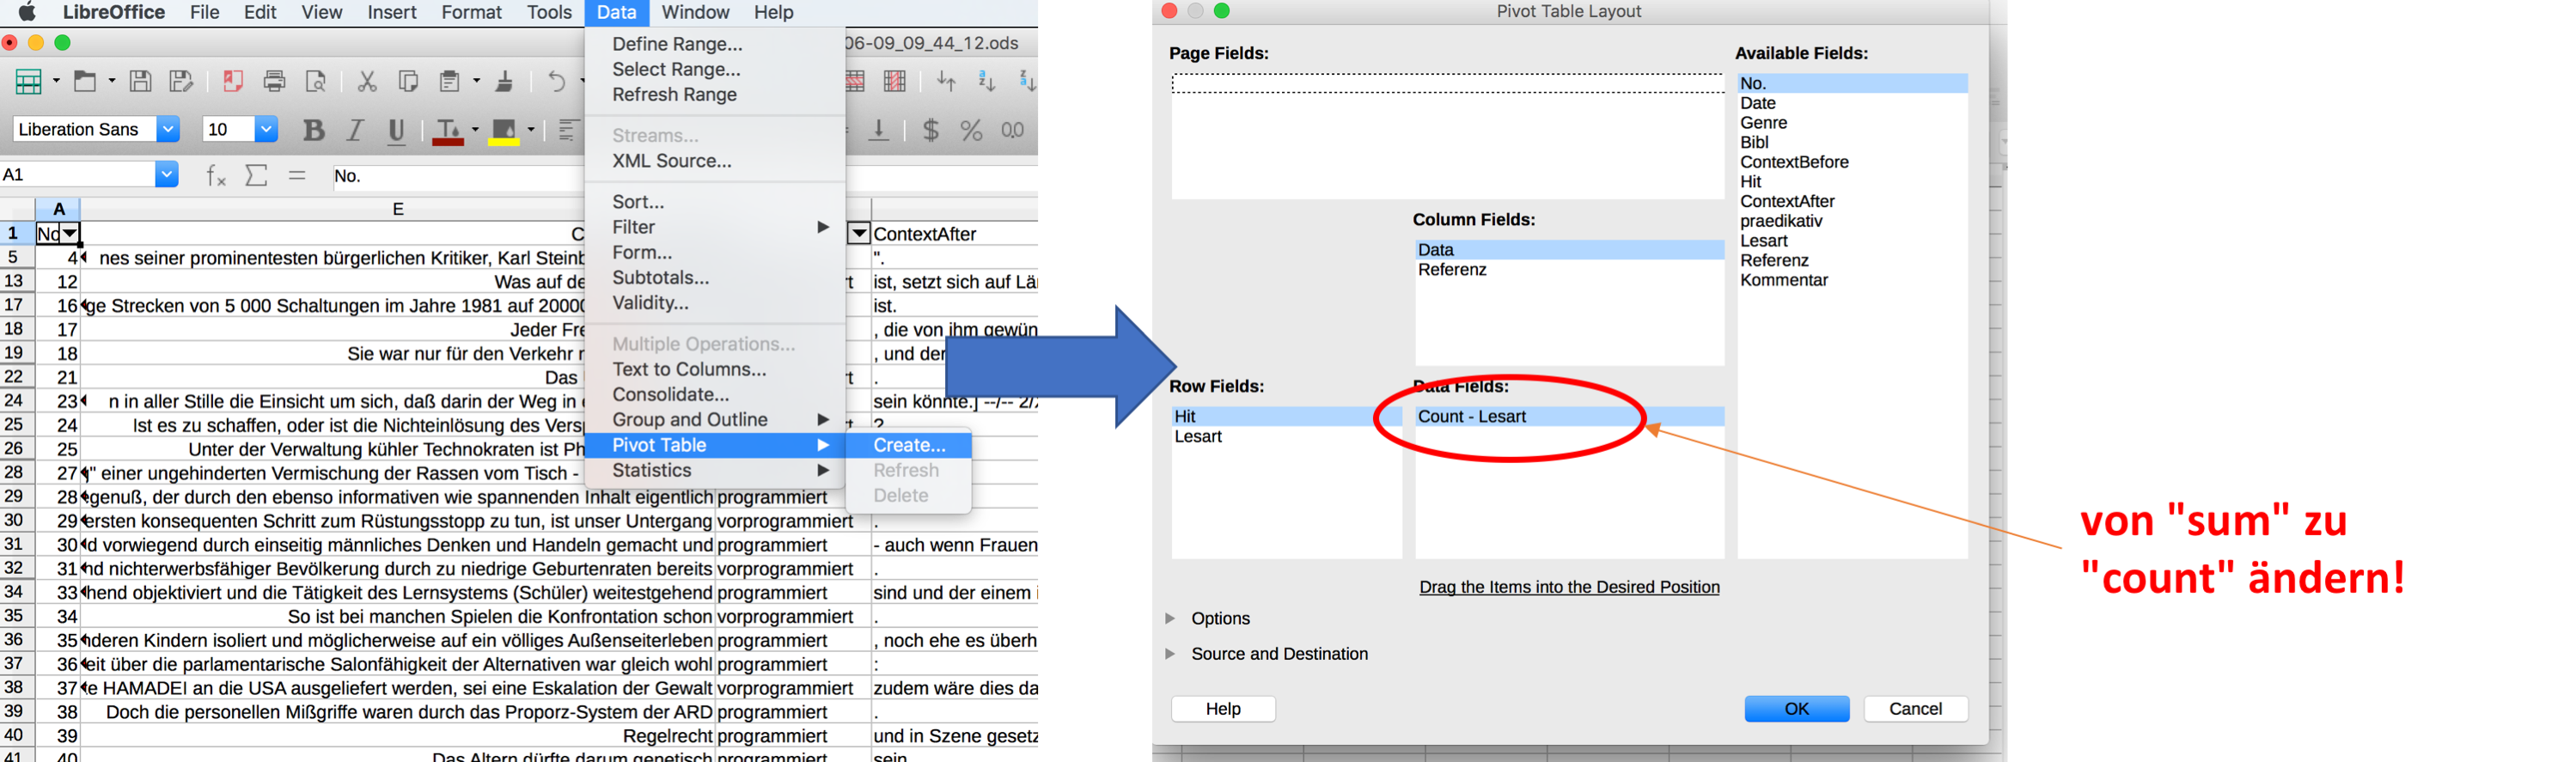
\includegraphics[width=6.66in]{docs/fig/calc_pivot} \caption{Erstellen einer Pivot-Tabelle in Calc.}\label{fig:calcpivot}
\end{figure}

Beim Erstellen der Pivot-Tabelle können wir in den ausklappbaren
Optionen auch auswählen, dass wir keine Zeilen- und Spaltensummen sehen
wollen (die brauchen wir nicht, zumal sie dann ggf. auch in den auf der
Tabelle basierenden Visualisierungen dargestellt werden und da nur
verwirren), aber dass wir Filter setzen möchten. Wenn wir nun auf OK
klicken, sehen wir die Pivot-Tabelle, oberhalb derer sich ein
\enquote{Filter}-Feld befindet, auf das wir doppelklicken können, um
durch Auswählen des Attribut-Wert-Paars \enquote{praedikativ = y} die
Tabelle so zu filtern, dass nur die prädikativen Belege angezeigt
werden.

Mit Hilfe der Tabelle können wir nun die Verteilung auch visualisiern,
z.B. mit einem Balkendiagramm.\footnote{Vgl. jedoch den Caveat in der
  vorherigen Fußnote.} Das ist über Insert \textgreater{} Chart möglich.
Hier haben wir die Wahl zwischen mehreren Optionen und wählen ein sog.
gestapeltes Balkendiagramm, das die prozentuale Verteilung anzeigt. Die
einzelnen Schritte sind in \ref{fig:calcchart} dargestellt.

\begin{figure}
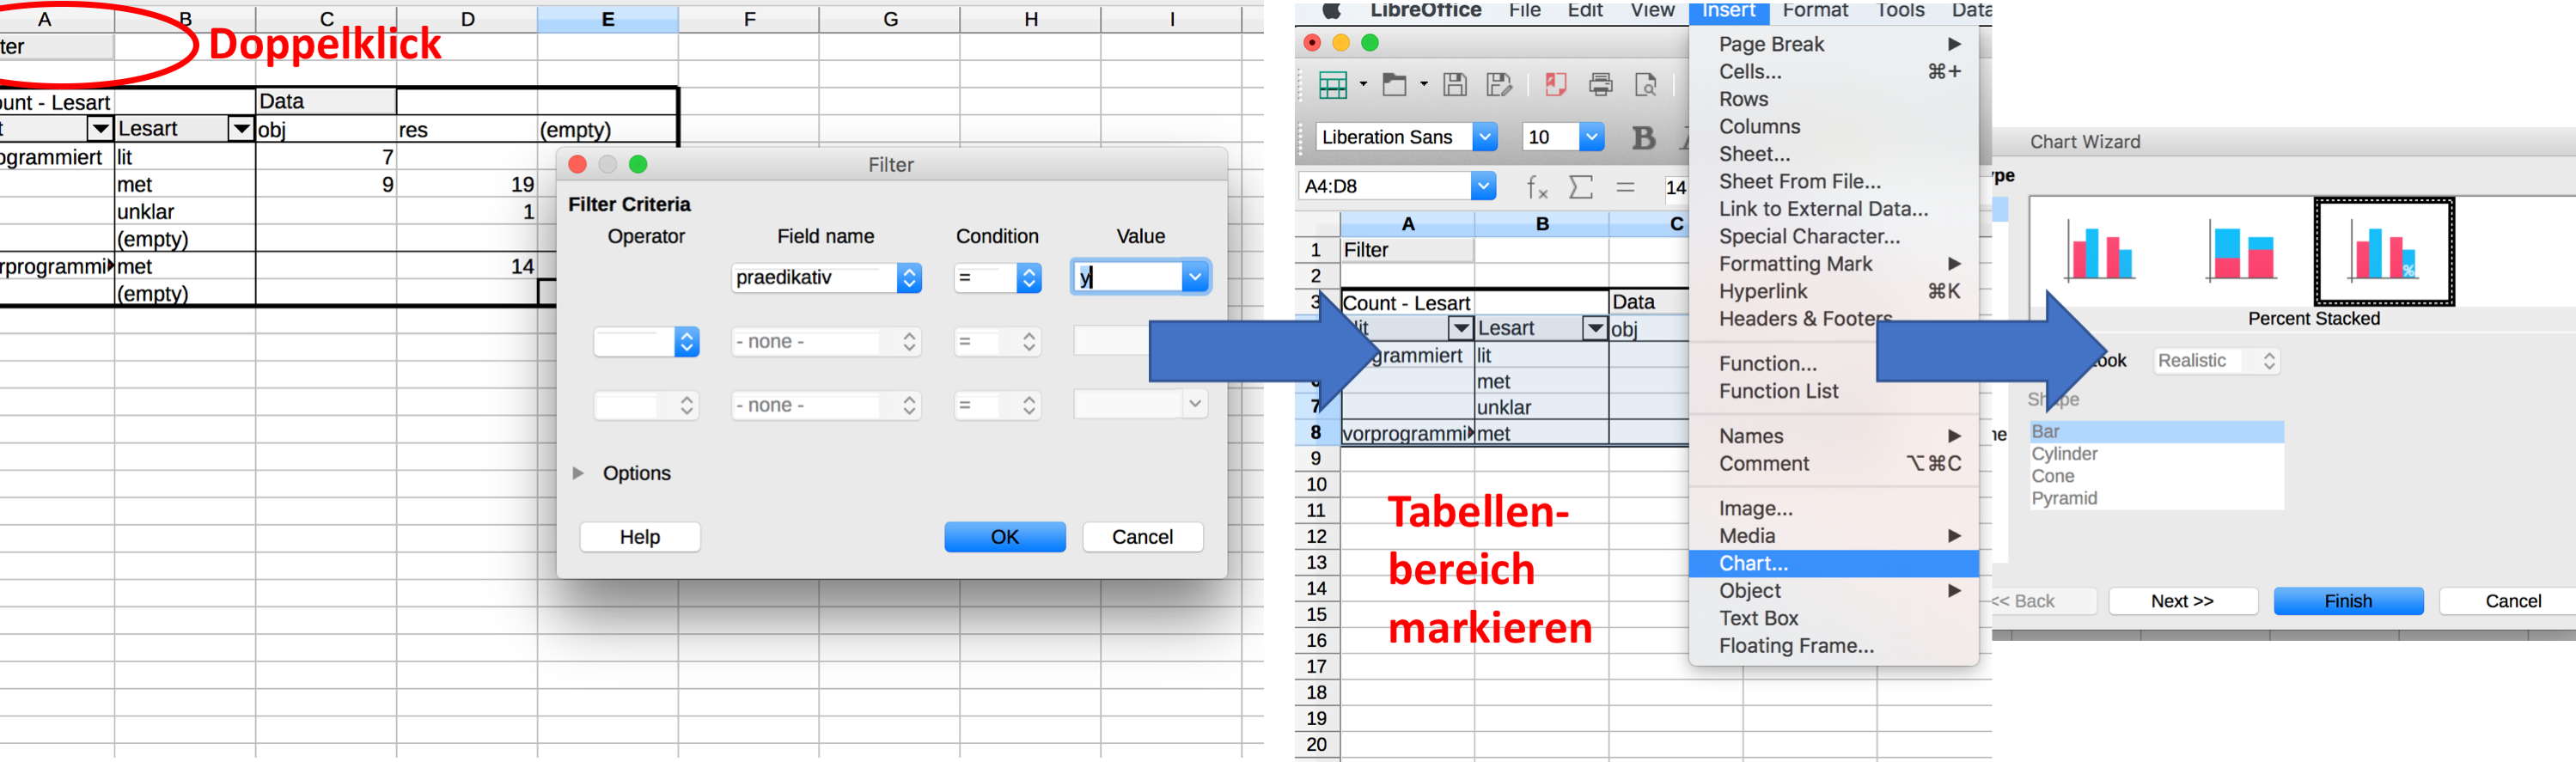
\includegraphics[width=6.66in]{docs/fig/calc_chart} \caption{Erstellen einer Pivot-Tabelle in Calc.}\label{fig:calcchart}
\end{figure}

Im Gegensatz zu Excel bietet Calc derzeit leider keine Möglichkeit, sich
in Pivot-Tabellen Nullwerte anzeigen zu lassen. Das heißt, wenn wir im
Balkendiagramm die Kategorien \enquote{lit} und \enquote{unklar} auch
für \emph{vorpgrammiert} sehen wollen, um das Diagramm symmetrisch zu
halten, müssen wir sie irgendwie manuell einfügen, weil für
\emph{vorprogrammiert} ja nur metaphorische Lesarten belegt sind. Einen
sehr uneleganten, aber funktionierenden Workaround zeigt
\ref{fig:calcchart2}: Weil wir an der Pivot-Tabelle selbst nichts
verändern können, copy\&pasten wir sie an eine andere Stelle im
Arbeitsblatt und ergänzen die fehlenden Kategorien manuell. Das ist
zwar, wie es ein User in einem Frage-und-Antwort-Forum zu diesem Thema
sehr schön formuliert hat, weniger eine Lösung als eine Kapitulation,
aber zumindest für diesen recht überschaubaren Datensatz funktioniert
der Ansatz.

\begin{figure}
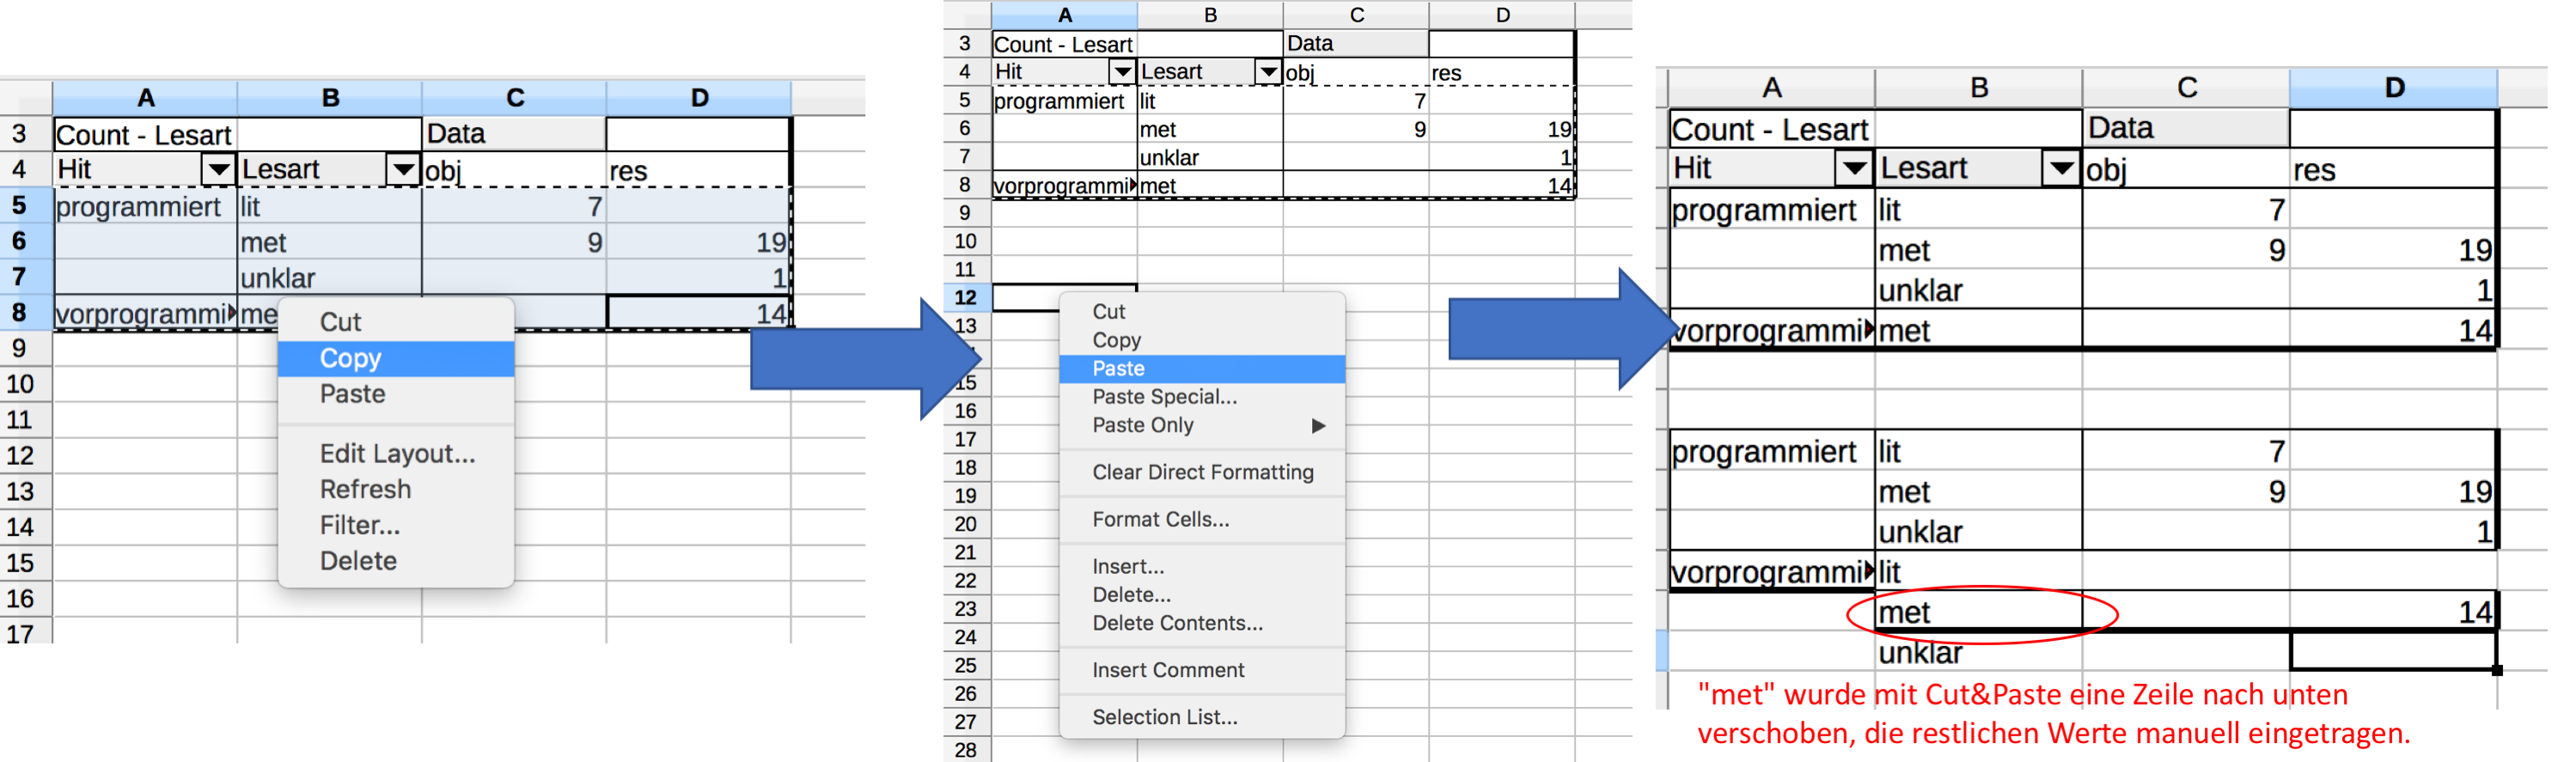
\includegraphics[width=6.66in]{docs/fig/calc_chart2} \caption{Erstellen einer Pivot-Tabelle mit Nullwerten in Calc (Workaround).}\label{fig:calcchart2}
\end{figure}

Zuletzt wollen wir die Balken noch mit Labels versehen, d.h. wir wollen
die absoluten Werte auf den Balken anzeigen. Auch hier kann Excel etwas
mehr als Calc, und wir müssen etwas tricksen, um die absoluten Werte
anzeigen zu lassen. Mit Rechtsklick auf einen der Balken \textgreater{}
Insert Data Labels können wir zunächst die Labels anzeigen lassen, sehen
aber erstens keine absoluten Werte, sondern Prozentwerte, und zweitens
absurde Prozentwerte, weil Calc offenbar die Zahlen in der Tabelle für
relative Werte hält. Mit Doppelklick auf eines der Labels können wir
jedoch das Zahlenformat ändern und angeben, dass wir die Labels einfach
als \enquote{Text} angezeigt bekommen wollen -- also einfach das, was in
der Pivot-Tabelle selbst steht (s. Fig. \ref{fig:calcdatalabels}).

\begin{figure}
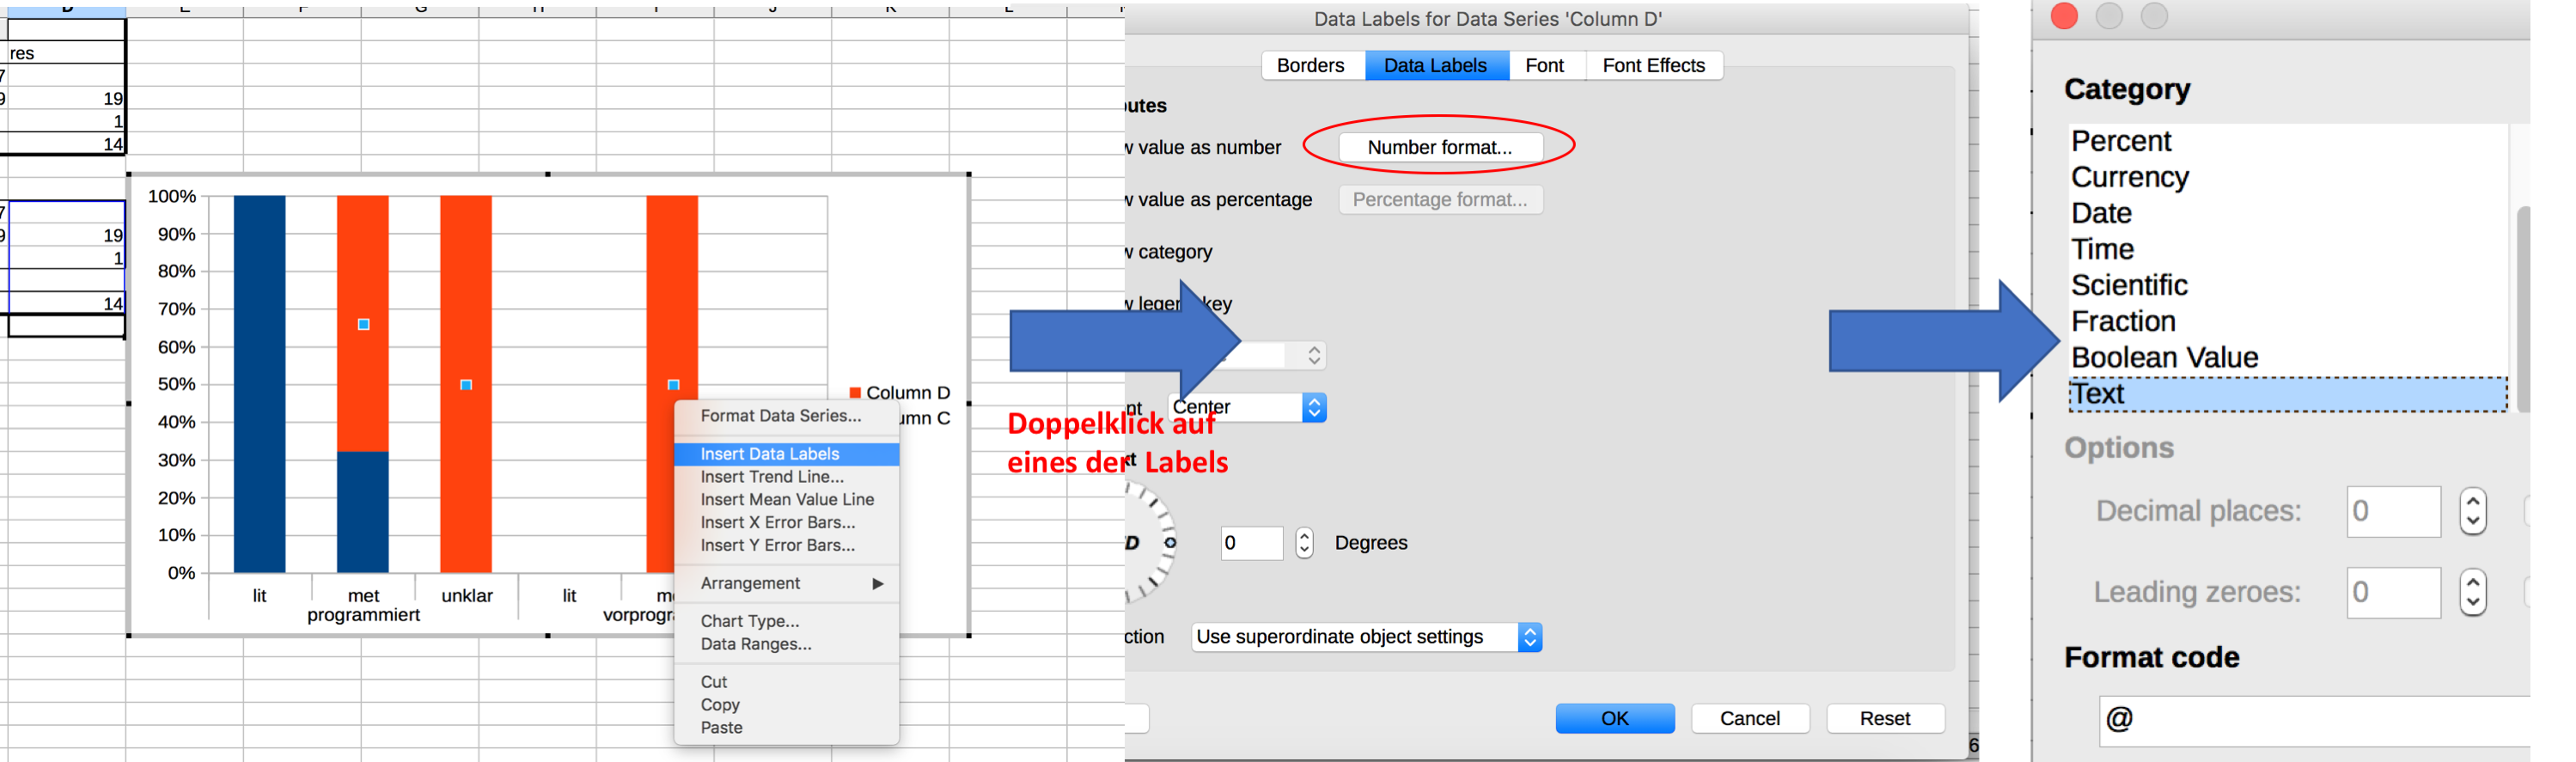
\includegraphics[width=6.66in]{docs/fig/calc_datalabels} \caption{Einfügen von Data labels in Calc.}\label{fig:calcdatalabels}
\end{figure}

\section{Und nun\ldots{}?}\label{und-nun}

Fassen wir kurz die wesentlichen Schritte zusammen, die wir uns in
diesem Tutorial näher angeschaut haben:

\begin{itemize}
\tightlist
\item
  Zunächst haben wir eine Fragestellung formuliert und sie
  korpuslinguistisch operationalisiert.
\item
  Wir haben Daten erhoben, indem wir im DWDS-Kernkorpus nach den beiden
  Wortformen, die uns interessieren, gesucht haben. Wir haben diese
  Daten exportiert und haben gesehen, wie man sie in ein
  Tabellenkalkulationsprogramm einliest.
\item
  Anschließend haben wir die Daten mit grammatischen und semantischen
  Annotationen versehen.
\item
  Zuletzt haben wir die Daten ausgewertet und visualisiert.
\end{itemize}

Das allein macht natürlich noch keine gute linguistische Studie aus. Wir
müssen uns jezt überlegen, wie die Daten zu interpretieren sind. Nicht
zuletzt müssen wir aber auch unser Vorgehen kritisch hinterfragen und
überlegen, welche Unzulänglichkeiten es möglicherweise mit sich bringt.

\subsection{Interpretation und
Einordnung}\label{interpretation-und-einordnung}

Fangen wir mit dem ersten Punkt an, der Interpretation: In unseren Daten
wird \emph{vorprogrammiert} ausschließlich im metaphorischen Sinn
verwendet und nur dann, wenn auf Resultate Bezug genommen wird. Das
untermauert unsere Annahme, dass \emph{vorpgrogrammiert} gegenüber
\emph{programmiert} eine bestimmte semantische Nische einnimmt
(wenngleich es in dieser Nische durchaus stark mit der Variante ohne die
Partikel \emph{vor-} konkurriert).

Auch werden Sie sich gefragt haben, ob denn das hier durchgearbeitete
Beispiel wirklich Stoff für z.B. eine ganze Seminararbeit bietet, wo wir
doch am Ende der langwierigen Korpusrecherche nicht viel mehr bekommen
haben als ein relativ simples Balkendiagramm. (Formulieren Sie diesen
Satz gerne etwas griffiger, damit Sie ihn sich auf ein T-Shirt drucken
lassen können.)

Auch wenn das hier besprochene Beispiel durchaus noch ausbaufähig ist
(siehe
\protect\hyperlink{methodenkritik-und-offene-fragen}{Methodenkritik}),
bietet es meines Erachtens doch genug Stoff für eine gute Hausarbeit,
sofern man die Korpusanalyse in eine gute theoretische Diskussion
einbettet und die hier vorgenommene quantitative Analyse vielleicht noch
durch die qualitative Analyse von Einzelbelegen ergänzt. Das könnte zum
Beispiel so aussehen, dass man sich zunächst in einem Theorieteil mit
der semantischen Entwicklung von (nahe-)synonymen Wörtern befasst und
dann am Beispiel von \emph{(vor)programmiert} der Frage nachgeht, ob die
Varianten mit und ohne Partikel unterschiedlich gebraucht werden, also
unterschiedliche semantische \enquote{Nischen} ausfüllen. In einem
Methodenteil kann man dann die Annotationskriterien offenlegen, ggf.
Problemfälle schildern und aufzeigen, wie sie gelöst wurden. Hier kann
man auch schon die Grenzen des gewählten Vorgehens ansprechen, auf die
wir im nächsten Abschnitt noch näher eingehen werden. Es folgen die
quantitative Analyse und die Diskussion der Ergebnisse vor dem
Hintergrund der Forschungsfrage, die gerne mit der qualitativen Analyse
von Korpusbelegen gespickt sein darf. In einem Schlussteil werden dann
die Ergebnisse zusammengefasst, und es werden Desiderata für zukünftige
Forschungen aufgezeigt -- ein Punkt, auf den wir ebenfalls im nächsten
Abschnitt noch eingehen werden.

\hypertarget{methodenkritik-und-offene-fragen}{\subsection{Methodenkritik
und offene Fragen}\label{methodenkritik-und-offene-fragen}}

Das führt uns zur Methodenkritik: Wie belastbar sind unsere Ergebnisse?
Hier ist als möglicherweise problematischer Punkt zunächst die
Stichprobengröße zu nennen. Im DWDS-Kernkorpus haben wir gerade einmal
88 Treffer gefunden, von denen nur rund 50 die prädikative Verwendung
instanziieren, die uns interessiert. Insofern wäre zu fragen, ob wir
möglicherweise besser ein anderes Korpus wählen sollten.

 ‣ \textbf{Zur Stichprobengröße}

Zur Frage nach der Stichprobengröße zitiere ich mich ausnahmsweise mal
selbst:

\begin{quote}
Die wahrscheinlich am häufigsten gestellte Frage von Studierenden, die
zum ersten Mal korpuslinguistisch arbeiten, ist: „Wie groß muss meine
Stichprobe sein?`` Darauf gibt es leider keine pauschale Antwort. Es
gibt keine feste Untergrenze, ab der eine Stichprobe repräsentativ ist
(zumal es „echte`` Repräsentativität in dem Sinne, dass die Stichprobe
ein ganz genaues Abbild der Grundgesamtheit, nur eben im Kleinen,
darstellt, ohnehin nicht geben kann). Die Wahl der Stichprobengröße ist
also von mehreren ganz praktischen Faktoren abhängig, unter anderem:
\end{quote}

\begin{quote}
\begin{enumerate}
\def\labelenumi{\alph{enumi})}
\tightlist
\item
  Wie werden die Daten annotiert? Sehr viele Annotationen, die noch dazu
  erfordern, dass der Kontext mit einbezogen wird, sind zeitaufwendig
  und rechtfertigen eine kleinere Stichprobe. Arbeitet man dagegen nur
  mit den reinen Type- und Tokenfrequenzen, ohne eigene Annotationen
  hinzuzufügen, gibt es keinen Grund, überhaupt eine Stichprobe zu
  nehmen. In diesem Fall kann man gleich alle Daten mit einbeziehen.
\item
  Wie werden die Daten ausgewertet? In manchen Fällen kann man schon mit
  100 Belegen aussagekräftige Ergebnisse erzielen. Aber wenn man ein
  Korpus diachron auswerten möchte, das in 10 Zeitschnitte unterteilt
  ist, sind 100 Belege offensichtlich zu wenig -- denn dann hat man bei
  gleicher Verteilung gerade einmal 10 Belege pro Zeitschnitt!
\end{enumerate}
\end{quote}

\begin{quote}
Für die ersten Gehversuche z.B. in Seminararbeiten empfehle ich in der
Regel, mit 100 bis 500 Belegen zu arbeiten. In den meisten Fällen genügt
das, um Tendenzen aufzuzeigen, und ist vom Arbeitsaufwand her auch für
AnfägerInnen bewältigbar. Aus den obigen Überlegungen sollte jedoch klar
geworden sein, dass diese Zahlen völlig willkürlich sind.
\end{quote}

\hfill --- aus: Hartmann, Stefan. 2018. Deutsche Sprachgeschichte.
Grundzüge und Methoden. Tübingen: Francke, S. 206

Weiterhin müssen wir bedenken, dass wir die Verteilung der Daten nur
relativ oberflächlich ausgewertet haben. Streng genommen müssten wir
eine Reihe von möglicherweise problematischen Aspekten zusätzlich
bedenken, denn bei Korpusdaten gibt es immer viele Faktoren, die zu
unerwünschten Verzerrungen führen können. So können viele verschiedene
Belege von der gleichen Person oder gar aus dem gleichen Text stammen.
Tab. \ref{tab:textverteilung} zeigt, dass 16 Belege in unserer
Konkordanz, wenig überraschend, aus dem \enquote{Lexikon der Informatik}
stammen\ldots{} In der modernen Korpuslinguistik tendiert man daher
dazu, statistische Methoden zu verwenden, mit denen man solche Variablen
mit einbeziehen kann.

\begin{table}[t]

\caption{\label{tab:textverteilung}Texte in der Konkordanz, die mehr als einen Beleg für (vor)programmiert enthalten}
\centering
\resizebox{\linewidth}{!}{
\begin{tabular}{lr}
\toprule
Text & Belege\\
\midrule
Rechenberg, Peter: Was ist Informatik?, München: Hanser 1994 [1991] & 16\\
Klee, Ernst: Behinderten-Report, Frankfurt a. M.: Fischer Taschenbuch-Verl. 1981 [1974] & 3\\
Alt, Franz: Liebe ist möglich, München: Piper 1985 & 2\\
Archiv der Gegenwart, 2001 [1975] & 2\\
Bädekerl, Klaus: Werthers Freundin. In: Hoffmann, Raoul (Hg.) Auf Live und Tod, München: Dt. Taschenbuch-Verl. 1983 [1979] & 2\\
\addlinespace
Die Zeit, 22.07.1999, Nr. 30 & 2\\
Jung, Mathias: Der militärisch-industrielle Komplex. In: Haug, Hans-Jürgen u. Maessen, Hubert (Hgg.) Kriegsdienstverweigerer - Gegen die Militarisierung der Gesellschaft, Frankfurt a. M.: Fischer 1971 & 2\\
Ketman, Per u. Wissmach, Andreas: DDR - ein Reisebuch in den Alltag, Reinbek bei Hamburg: Rowohlt 1986 & 2\\
Loriot [d.i. Vicco von Bülow]: Sehr verehrte Damen und Herren ..., Zürich: Diogenes 1993 & 2\\
Wilberg, Gerlinde M.: Zeit für uns, München: Frauenbuchverl. 1979 & 2\\
\bottomrule
\end{tabular}}
\end{table}

Das Stichwort \enquote{statistische Methoden} bringt uns zu einem
weiteren Punkt, den wir hier explizit \textbf{nicht} behandelt haben:
Wir haben uns nicht mit der Frage beschäftigt, ob der Unterschied
zwischen den untersuchten Variablen in irgendeiner Weise statistisch
signifikant ist (und was statistische Signifikanz überhaupt bedeutet).
In unserem Beispiel war der Unterschied zwischen \emph{programmiert} und
\emph{vorprogrammiert} erfreulicherweise so klar und offensichtlich,
dass es einer statistischen Analyse nicht wirklich bedarf. Wenn Sie sich
weiter damit beschäftigen wollen, empfehle ich die Lektüre einer der
einschlägigen Einführungen.

 ‣ \textbf{Zum Weiterlesen: Statistik für LinguistInnen}

Hier eine Auswahl an deutsch- und englischsprachigen Einführungswerken
in die Statistik, die sich explizit an Linguist*innen richten
(chronologisch geordnet):

\begin{itemize}
\item
  Desagulier, Guillaume. 2017. Corpus linguistics and statistics with R:
  introduction to quantitative methods in linguistics. New York, NY:
  Springer.
\item
  Levshina, Natalia. 2015. How to do linguistics with R. Data
  exploration and statistical analysis. Amsterdam, Philadelphia: John
  Benjamins.
\item
  Gries, Stefan Th. 2013. Statistics for Linguistics with R: A Practical
  Introduction. 2nd ed. Berlin, New York: De Gruyter.
\item
  Meindl, Claudia. 2011. Methodik für Linguisten: Eine Einführung in
  Statistik und Versuchsplanung. Tübingen: Narr.
\item
  Baayen, R. H. 2008. Analyzing Linguistic Data. A Practical
  Introduction to Statistics using R. Cambridge: Cambridge University
  Press.
\item
  Butler, Christopher. 1985. Statistics in Linguistics. Oxford:
  Blackwell.
\end{itemize}

Über die Methodenkritik hinaus können wir natürlich auch Desiderata
formulieren, also fragen, in welche Richtung wir weiterforschen können.
So haben wir uns in unserem Beispiel auf prädikative Verwendungen von
\emph{(vor)programmiert} beschränkt. Das war eine sinnvolle und gut
begründbare Vorentscheidung, um den Skopus der Untersuchung
einzugrenzen, und deshalb nichts, was wir im Rahmen der Methodenkritik
hinterfragen sollten. Gleichwohl können wir die Frage stellen, wie sich
wohl die flektierten Formen von \emph{(vor)programmieren} verhalten und
ob sich ähnliche Tendenzen auch hier aufzeigen lassen.

Es bietet sich immer an, eine Arbeit mit solchen Desiderata
abzuschließen, denn keine Forschungsfrage ist je vollständig
beantwortet, und jede (Teil-)Antwort wirft nahezu zwangsläufig neue
Fragen auf.


\end{document}
